\documentclass[11pt, a4paper, oneside]{book}

% URLs and hyperlinks ---------------------------------------
\usepackage{hyperref}
\hypersetup{
	colorlinks=true,
	linkcolor=blue,
	filecolor=magenta,      
	urlcolor=blue,
}
\usepackage{xurl}
%---------------------------------------------------

% adjust a verrrrry big table -------------------------------
\usepackage{adjustbox}
% -----------------------------------------------------------

% titlepage -------------------------------------------------
\usepackage{pdfpages}
%------------------------------------------------------------
\usepackage{booktabs}
\usepackage{rotating} % برای چرخاندن جدول
\usepackage{amssymb}
\usepackage{amsmath}

% page headers -------------------------------------------------
\usepackage{fancyhdr}
\fancypagestyle{plain}{\fancyhf{}\renewcommand{\headrulewidth}{0pt}}
\pagestyle{fancy}
\fancyhf{}% Clear header/footer
\fancyhead[L]{\nouppercase\leftmark}
\fancyhead[R]{\thepage}
%---------------------------------------------------------------

% tables -------------------------------------------------------
\usepackage{float}
\usepackage{multirow}
\renewcommand{\arraystretch}{1.23}
% ---------------------------------------------------------------------

\usepackage{xepersian}
\settextfont{Yas} %B Nazanin
\setdigitfont{Yas} %Times New Roman
\setlatintextfont{Yas} %Times New Roman

\begin{document}
	\renewcommand{\bibname}{مراجع}
	\frontmatter
	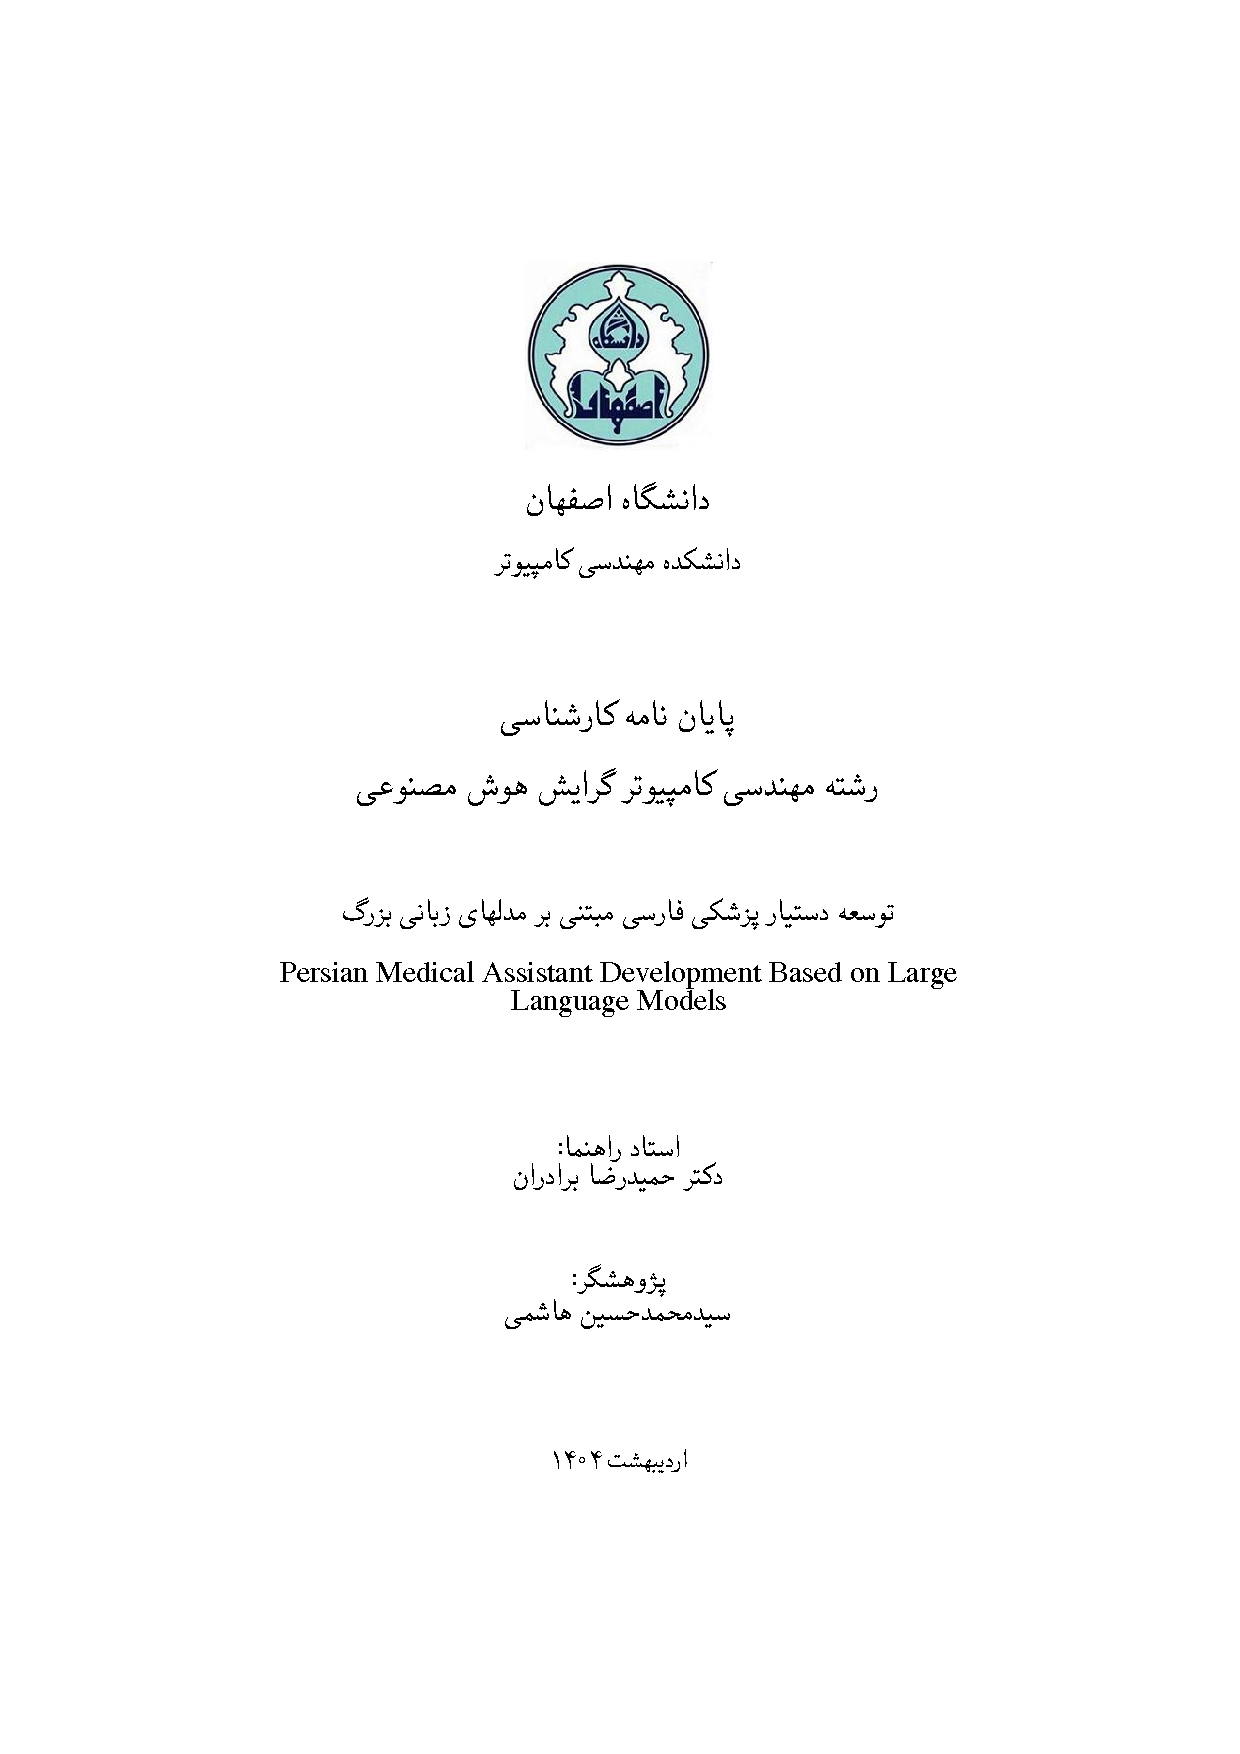
\includepdf{../title-page/title}
	
	\clearpage \thispagestyle{plain}\mbox{}\clearpage
	
	\clearpage
	\begin{center}
		
\includegraphics[width=10cm]{../images/image002}
	\end{center}  
	\thispagestyle{plain}\mbox{} 
	\clearpage
	
	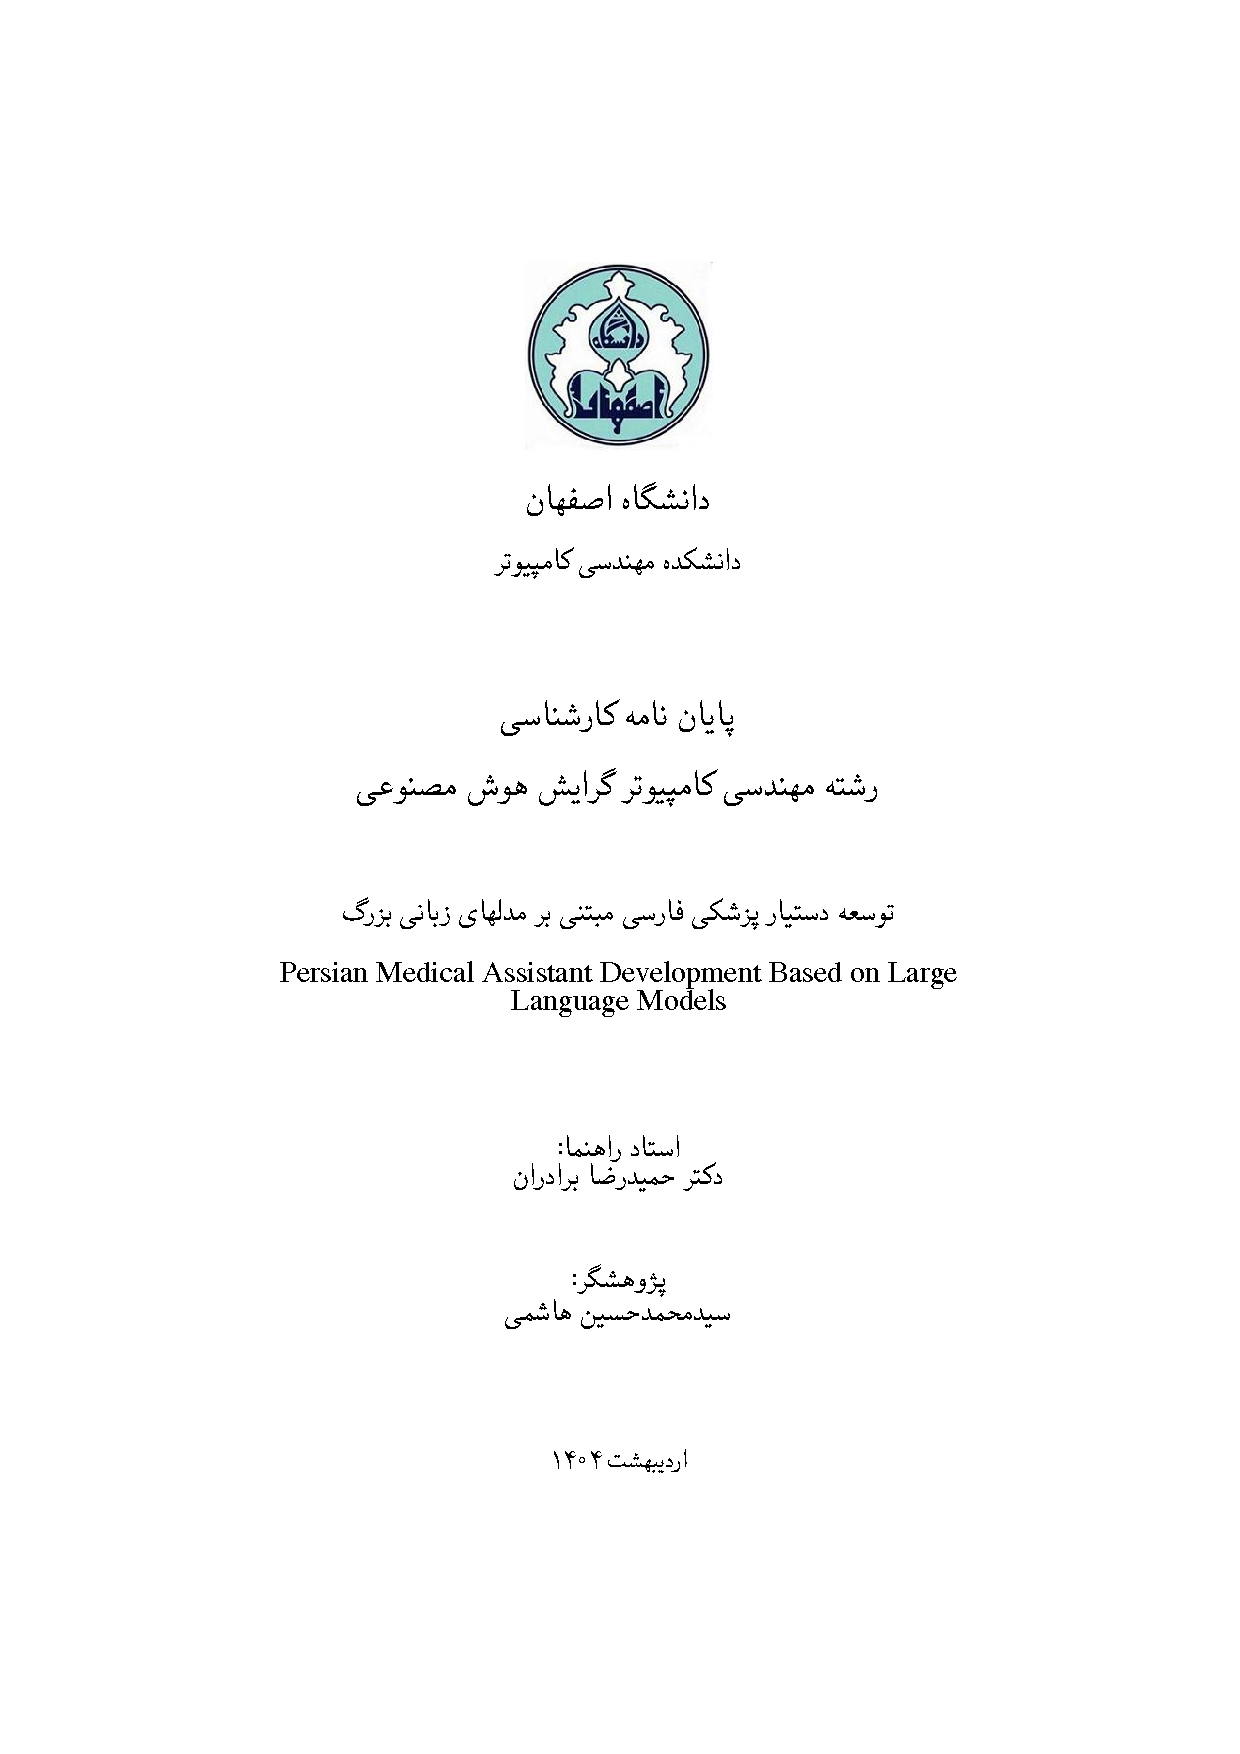
\includepdf{../title-page/title}
	
	\newpage
	
	\section*{چکیده}

			با معرفس مدل‌های زبانی بزرگ مانند \lr{ChatGPT} که در بسیاری از حوزه‌های علمی دانش خوبی دارند به مرور نیاز به مدل‌های متخصص نیز ایجاد شد. علاوه بر این مدل‌هایی از این قبیل دو مشکل اساسی دارند که به آن می‌پردازیم.
			
			یکی از بزرگ‌ترین مشکلات این مدل‌ها این است که تضمینی برای اینکه سوالات و داده‌های ارسالی را ذخیره نکنند وجود ندارد. در داده‌هایی مانند داده‌های پزشکی که حساسیت بسیار بالایی دارد این اتفاق پیامدهای بسیار بدی می‌تواند داشته باشد.
			
			دومین مشکل، مشکل وزن مدل‌هاست، ما نیاز داریم مدل‌ها را در سخت افزارهایی بسیار محدودتر از \lr{OpenAI} و سایر شرکت‌های این حوزه اجرا کنیم، چون همانطور که اشاره شد برای اینکه اطلاعات در سیستم‌های خارجی ذخیره نشود نیاز است که مدل‌ها در سخت افزارهای محلی و ضعیف هم به خوبی کار کند.
			
			با توجه به مشکلات اشاره شده هدف این پروژه توسعه مدل متخصص پزشکی است که در آن دانش داخلی و خارجی مدل ارتقا داده می‌شود و از تکنیک‌های \lr{Prompt engineering} نیز برای افزایش دقت پاسخدهی استفاده می‌کنیم.
			
	\newpage
	
	\tableofcontents	
	\newpage
	\listoffigures
	\listoftables
	\newpage
	\mainmatter
	\chapter{مقدمه}
		
			مدل‌های زبانی بزرگ\LTRfootnote{Large Language Models} به‌عنوان یکی از پیشرفت‌های برجسته در حوزه هوش مصنوعی و پردازش زبان طبیعی (NLP) شناخته می‌شوند. این مدل‌ها، که بر پایه معماری قدرتمند ترنسفورمر طراحی شده‌اند، توانایی درک و تولید متن را با دقت بالا دارند. معماری ترنسفورمر، با استفاده از مکانیزم توجه\LTRfootnote{Attention Mechanism}، وابستگی‌های میان کلمات در متن را یاد می‌گیرد و امکان تحلیل دقیق آن را فراهم می‌کند. این مدل‌ها ابتدا متن ورودی را به توکن‌هایی تبدیل می‌کنند و سپس هر توکن را به یک بردار عددی در فضای برداری تبدیل می‌کنند. مکانیزم \lr{Self-Attention} وابستگی میان توکن‌ها را محاسبه کرده و اطلاعات را به شکلی سازمان‌یافته پردازش می‌کند. همچنین، استفاده از \lr{Positional Encoding} ترتیب کلمات را حفظ کرده و مدل را قادر می‌سازد تا توالی‌های طولانی را درک کند. \cite{vaswani_attention_2023}
			
			این مدل‌ها در دو مرحله اصلی آموزش داده می‌شوند. مرحله اول پیش‌آموزش\LTRfootnote{Pretraining} است که در آن مدل با استفاده از داده‌های متنی عظیم، ساختار و معنای زبان را یاد می‌گیرد. در مرحله دوم، مدل از طریق تنظیم دقیق\LTRfootnote{Fine-Tuning} روی داده‌های خاص یک کاربرد مانند ترجمه، چت یا خلاصه‌سازی متن، تنظیم می‌شود. برخی از مدل‌ها نیزعلاوه بر فاین‌تیونینگ، از روش‌هایی مانند یادگیری تقویتی با بازخورد انسانی\LTRfootnote{Reinforcement Learning from Human Feedback (RLHF)} بهره می‌گیرند تا کیفیت پاسخ‌ها را بهبود بخشند. به کمک این رویکردها، مدل‌های زبانی توانسته‌اند در تولید متون طبیعی، درک زبان انسانی و انجام وظایف پیچیده‌ای نظیر پاسخ‌گویی به پرسش‌ها و تحلیل داده‌های متنی عملکرد بی‌نظیری دارند .
			
			با پیشرفت مدل‌های زبانی، رویکردهای جدیدی مانند \lr{RAG}\LTRfootnote{Retrieval-Augmented Generation} نیز ظهور کرده‌اند. \lr{RAG} با ترکیب مدل‌های زبانی و پایگاه‌های داده خارجی، عملکرد مدل‌ها را بهبود می‌بخشد.\cite{lewis_retrieval-augmented_2021} به‌جای اتکا به پارامترهای داخلی، \lr{RAG} اطلاعات دقیق و به‌روز را از منابع خارجی که در ساختارهای \lr{Vector Database} یا \lr{Graph Database} ذخیره شده‌اند بازیابی و در اختیار مدل فرار می‌دهد. \lr{Vector Database} با ذخیره داده‌ها به شکل بردارهای تعبیه‌شده، امکان جستجوی سریع بر اساس مشابهت معنایی را فراهم می‌کند که باعث بهبود پاسخگویی در سوالات کلی می‌شود، در حالی که \lr{Graph Database} برای مدل‌سازی روابط پیچیده و شبکه‌های دانش مناسب است. این ترکیب به مدل اجازه می‌دهد تا در پاسخ به سوالات پیچیده و جزئی که نیاز به فراهم کردن اطلاعات دقیق‌تر و جزئی‌تر دارند، توانایی بیشتری از خود نشان دهد. \cite{edge_local_2024} \cite{guo_lightrag_2024}
			
			یکی دیگر از مباحث کلیدی در بهبود عملکرد مدل‌های زبانی، \lr{Prompt Engineering} یا هدایت مدل به تولید پاسخ‌های دقیق‌تر با استفاده از ورودی که به مدل داده می‌شود است. در این مبحث توانایی مدل را بدون تنظیم مدل روی حوزه خاص ارتقا می‌دهیم. \cite{brown_language_2020}
			رویکردهای متنوعی در این زمینه توسعه یافته‌اند. به‌عنوان مثال، در روش زنجیره تفکر\LTRfootnote{Chain of Thought (CoT)} که مدل را به ارائه پاسخ‌هایی گام‌به‌گام هدایت می‌کند که برای مسائل پیچیده مانند ریاضیات یا استدلال منطقی وادار می‌کند که در آن دقیقا مانند ما انسان‌ها که مسائل را بخش بخش حل می‌کنیم سوال را به بخش‌های مختلف و ساده‌تری تقسیم می‌کند که باعث می‌شود مدل بتواند راحت‌تر و دقیق تر به سوالات پاسخ بدهد. استفاده از این تکنیک‌های مانند این، به‌ویژه در وظایفی مانند پرسش و پاسخ پیچیده یا برنامه‌ریزی، به‌طور قابل‌توجهی کیفیت و دقت خروجی‌ها را افزایش می‌دهد. \cite{wang_prompt_2024} \cite{wei_chain--thought_2023}
			
			در نهایت مدل‌ها را می‌توان با استفاده این روش‌ها به متخصصی در حوزه خاص تبدیل کرد که سوالات مختلف را پاسخ بدهد. و در این پروژه هدف من این است که با بررسی و استفاده از این روش‌ها و موارد مشابه مدل زبانی تخصصی در حوزه پزشکی ایجاد کنم که به عنوان دستیار پزشکی به سوالات پزشکی به خوبی پاسخ دهد.
			روند انجام این پروژه بدین صورت است که ابتدا موارد مشابه بررسی می‌شوند و سپس به بررسی داده‌های موجود در این حوزه پرداخته می‌شود.
			
			پس از آن روش‌های ارزیابی مدل‌ها را بررسی و اقدام به ارزیابی مدل‌های فارسی می‌پردازم.
			سپس مدل قوی‌تر را در دو فاز دانش داخلی و خارجی ارتقا می‌دهم که خود ارتقای داخلی شامل \lr{SFT}\LTRfootnote{Supervised Fine-Tuning} و \lr{Alignment} است که ابتدا روش‌های موجود در هرکدام بررسی و مقایسه و بهترین روش انتخاب و روی مدل پیاده سازی می‌شود تا مدل پایه به دست آید. پس از آن به بررسی روش‌های موجود برای افزایش دانش داخلی یعنی انواع \lr{RAG} سیستم‌ها پرداخته می‌شود.
			پس از آن روش‌های \lr{prompt engineering} بررسی می‌شوند و پس از آن رابط کاربری ساده‌‌ای برای تعامل با مدل ایجاد می‌شود.
			در نهایت به امکانات دیگری که میتوان به این دستیار اضافه کرد پرداخته می‌شود که که به دلایل محدودیت‌های سخت افزاری و یا اطلاعاتی امکان انجام آن را نداشتم.
			
			
			
	\chapter{پژوهش‌های مشابه} \label{related_works}
	
		در این بخش پژوهش‌های مشابه که به صورت تخصصی در این حوزه انجام و منجر به ایجاد مدل زبانی تخصصی برای دستیار پزشکی شده‌اند را بررسی می‌کنیم.
	
		\section{\lr{Med-PaLM}}
			
			در این پژوهش به صورت هماهنگ بر توسعه و بهبود کاربرد مدل‌های زبانی بزرگ\LTRfootnote{LLMs} در حوزه پزشکی تمرکز دارند و با هم پیشرفت‌های چشمگیری در این زمینه نشان می‌دهند. در هر دو مقاله، از مدل‌های پیشرفته زبانی مانند \lr{PaLM} و \lr{Flan-PaLM }استفاده شده و نسخه‌های تخصصی این مدل‌ها، یعنی \lr{Med-PaLM} و \lr{Med-PaLM 2}، برای هم‌راستایی با نیازهای خاص پزشکی توسعه یافته‌اند. تلاش‌ها بر بهبود دقت، استدلال، و علمی بودن پاسخ‌ها متمرکز بوده است، که با استفاده از تکنیک‌هایی مانند زنجیره تفکر\LTRfootnote{CoT} و زنجیره تفکر خودسازگار\LTRfootnote{sc-CoT}، و تنظیم دستورالعمل ورودی به مدل انجام شد. برای ارزیابی عملکرد این مدل‌ها، معیار جامع \lr{MultiMedQA} شامل داده‌های متنوع چندگزینه‌ای و پاسخ‌های بلند توسعه یافته است. نتایج نشان داده که مدل‌های بهبودیافته می‌توانند در معیارهای مختلف مانند پاسخ‌دهی دقیق، کاهش محتوای نادرست، و پاسخ‌های معتبر عملکردی نزدیک به پزشکان داشته باشند. با این حال، هر دو مقاله بر چالش‌های باقی‌مانده مانند نیاز به داده‌های متنوع‌تر، تعصبات بالقوه، و ارزیابی در سناریوهای واقعی بالینی تأکید می‌کنند. این پژوهش‌ها به‌طور کلی گامی اساسی در جهت استفاده امن و مؤثر از مدل‌های زبانی در کاربردهای حساس پزشکی به شمار می‌آیند. \cite{singhal_large_2022} \cite{singhal_towards_2023}
			
		\section{\lr{Meditron}}
			این پژوهش به معرفی مدل‌های \lr{MEDITRON} که در دو مقیاس 7 و 70 میلیارد پارامتر ارائه شده‌اند می‌پردازد که با هدف بهبود دسترسی به دانش پزشکی و تقویت مدل‌های متن‌باز تخصصی در حوزه پزشکی ایجاد شده‌اند. این مدل‌ها با استفاده از معماری \lr{Llama-2} و آموزش کامل\LTRfootnote{Pre-train} بر روی داده‌های جامع پزشکی شامل مقالات \lr{PubMed}، دستورالعمل‌های بالینی، و داده‌های عمومی توسعه یافته‌اند. ارزیابی‌ها نشان داد که \lr{MEDITRON} در معیارهای اصلی پزشکی مانند \lr{MedQA} و \lr{PubMedQA} عملکردی بهتر از مدل‌های متن‌باز موجود دارد و در برخی موارد با مدل‌های تجاری بسیار بزرگ‌تر مانند \lr{GPT-4} رقابت می‌کند. همچنین، استفاده از روش‌های استنتاج پیشرفته مانند زنجیره استدلال \lr{(CoT)} و زنجیره استدلال با خودسازگاری \lr{(cs-CoT)} موجب بهبود قابل‌توجه عملکرد مدل شده است. انتشار متن‌باز ابزارها، کدها، و منابع این پژوهش، امکان ارزیابی واقعی مدل و توسعه بیشتر مدل‌های زبانی تخصصی در حوزه‌های مختلف، به‌ویژه پزشکی، را فراهم می‌کند. \cite{chen_meditron-70b_2023}
	
		\section{\lr{BioMistral}}
			این پژوهش به معرفی \lr{BioMistral 7B} می‌پردازد، یک مدل زبان بزرگ متن‌باز تخصصی برای حوزه پزشکی که با استفاده از مدل پایه \lr{Mistral 7B Instruct} و بازآموزی بر داده‌های علمی \lr{PubMed Central} توسعه یافته است. هدف از این پژوهش، ایجاد مدلی با عملکرد برتر در وظایف پزشکی در کنار حفظ قابلیت‌های عمومی مدل‌های زبان بزرگ است. ارزیابی مدل در یک معیار متشکل از ۱۰ وظیفه پرسش و پاسخ پزشکی در زبان انگلیسی بوده که پس از آن به ۷ زبان دیگر ترجمه و ارزیابی شد و نتایج به دست آمده نشان داد که \lr{BioMistral 7B} در بیشتر وظایف بر مدل‌های متن‌باز موجود برتری دارد و در برخی موارد به مدل‌های اختصاصی نزدیک می‌شود. همچنین، با استفاده از تکنیک‌های کوانتیزه‌سازی\LTRfootnote{Quantization} و ادغام مدل\LTRfootnote{Model Merging}، بهره‌وری و عملکرد آن بهبود یافته است. علاوه بر این، مدل در زبان‌های مختلف و ویژگی‌هایی مانند کالیبراسیون\LTRfootnote{Calibration} و حقیقت‌گرایی\LTRfootnote{Truthfulness} نیز ارزیابی شد و نتایج قابل قبولی ارائه کرد. در نهایت، این پژوهش به انتشار داده‌ها و مدل‌ها در پلتفرم‌های متن‌باز پرداخته و پیشنهادهایی برای بهبود قابلیت‌های چندزبانه و مکالمه‌ای مدل ارائه داده است. \cite{labrak_biomistral_2024}
		
		\section{\lr{Aloe}}
			مدل‌های \lr{Aloe} به‌عنوان مجموعه‌ای از مدل‌های متن‌باز برای کاربردهای پزشکی توسعه یافته‌اند. این فرایند با انتخاب مدل‌های پایه مناسب مانند \lr{Mistral-7B} و \lr{Llama 3-8B} آغاز شد و از طریق تنظیم‌دقیق\LTRfootnote{Supervised Fine-Tuning} با داده‌های عمومی و پزشکی بهینه‌سازی شده است. برای افزایش دقت، از داده‌های مصنوعی به سبک زنجیره تفکر\LTRfootnote{Chain of Thought} و تکنیک ادغام مدل‌ها استفاده شد که بدون افزایش اندازه مدل، عملکرد آن را بهبود بخشید. در مراحل بعدی، تنظیم ترجیحات انسانی با روش \lr{DPO} \LTRfootnote{Direct Preference Optimization} برای شناسایی و کاهش خطرات و پاسخ‌های مضر انجام گرفت. همچنین، تکنیک‌های پیشرفته طراحی ورودی مانند \lr{Medprompt} باعث افزایش چشمگیر دقت مدل در پاسخگویی به سوالات پزشکی شد. نسخه نهایی \lr{Llama3-Aloe-8B-Alpha} با تمرکز بر شفافیت، اخلاق و قابلیت بازتولید منتشر شد. \cite{gururajan_aloe_2024}
			
		
		\section{\lr{Meerkat}}
			مدل \lr{Meerkat} با هدف ایجاد یک سیستم هوش مصنوعی پزشکی متن‌باز با قابلیت استدلال زنجیری و پیشرفته توسعه یافت. این پروژه با انتخاب معماری‌های پیشرفته مانند \lr{Mistral-7B} و \lr{LLaMA-3} آغاز شد، که به دلیل قابلیت پردازش سریع و دقت بالا به عنوان پایه انتخاب شدند. سپس، با طراحی و تولید مجموعه داده‌های آموزشی متنوع، شامل داده‌های زنجیره‌ تفکر استخراج‌شده از 18 کتاب درسی پزشکی، مجموعه داده \lr{MedBooks-CoT-18} اماده شد و بیش از 78,000 سؤال تولیدشده توسط \lr{GPT-4}، مدل برای حل مسائل پیچیده پزشکی نیز آماده شد. برای افزایش توانایی مدل در پاسخ به سؤالات واقعی بالینی، از مجموعه داده‌های موجود مانند \lr{MedMCQA} و \lr{LiveQA} استفاده شد و داده‌های دیگری همچون \lr{ChatDoctor-cleaned} و \lr{MedQA-dialogue} برای تقویت قابلیت مکالمات چندمرحله‌ای طراحی شدند. این داده‌ها با استفاده از تکنیک‌های پیشرفته مانند \lr{FlashAttention} پردازش و آموزش مدل‌ها با استفاده از \lr{GPU}ها و \lr{TPU}ها انجام شد. مدل‌ها با معیارهای مختلف از جمله \lr{MedQA} و چالش‌های \lr{NEJM} ارزیابی شدند، که نتایج نشان داد \lr{Meerkat-7B} اولین مدل \lr{7B} بود که مرز نمره قبولی \lr{USMLE} را عبور کرد و \lr{Meerkat-70B} توانست با \lr{GPT-4} رقابت کند و حتی در برخی معیارها عملکرد بهتری داشته باشد. این رویکرد، ترکیبی از معماری‌های کارآمد، داده‌های آموزشی غنی، و روش‌های پیشرفته ارزیابی را به کار گرفت تا مدلی مؤثر و دقیق برای حل چالش‌های پزشکی ارائه دهد. \cite{kim_small_2024}
		
		\section{\lr{MedMobile}} \label{MedMobile}
			مدل \lr{MedMobile} با هدف ایجاد یک دستیار پزشکی کوچک، کم‌هزینه، و تخصصی توسعه یافت که بتواند روی دستگاه‌های همراه اجرا شود و نیازی به زیرساخت‌های محاسباتی پیچیده نداشته باشد. توسعه این مدل با استفاده از \lr{phi-3-mini} به عنوان مدل پایه انجام شد، مدلی متن‌باز با 3.8 میلیارد پارامتر که برای کاربرد در دستگاه‌های همراه مناسب بود. تیم تحقیقاتی با استفاده از مجموعه داده‌های پزشکی \lr{UltraMedical} شامل بیش از 400 هزار پرسش چندگزینه‌ای پزشکی، مدل را از طریق فرآیند تنظیم دقیق نظارت‌شده\LTRfootnote{SFT} آموزش دادند. این داده‌ها ترکیبی از نمونه‌های دستی (توسط متخصصان) و مصنوعی (ایجادشده توسط \lr{GPT-4} و منابع مرجع پزشکی) بودند. با استفاده از تکنیک‌های پیشرفته مانند زنجیره استدلال (CoT)، دانش و فرآیند استدلال منطقی GPT-4 به مدل کوچک‌تر منتقل شد. برای بهبود دقت، روش یادگیری جمعی\lr{Ensembling} به کار گرفته شد که چندین پاسخ را ترکیب کرده و دقیق‌ترین آن را انتخاب می‌کرد. علاوه بر این، دستورات ورودی مدل با ابزار \lr{TextGrad} بهینه‌سازی شدند، اما محدودیت‌های مربوط به پنجره متنی در مدل‌های کوچک باعث شد که استفاده از دستورات اضافی عملکرد مدل را کاهش دهد. همچنین، روش‌های دیگری مانند بازیابی مبتنی بر اطلاعات\LTRfootnote{RAG} و \lr{k-shot prompting} نیز آزمایش شدند، اما به دلیل پیچیدگی و افزایش طول ورودی، تاثیر قابل‌توجهی بر عملکرد نداشتند. در نهایت، \lr{MedMobile} با عملکرد 75.7٪ در آزمون \lr{MedQA (USMLE)} موفق شد به عنوان اولین مدل زیر 5 میلیارد پارامتر نمره قبولی در این آزمون را کسب کند، که این دستاورد نشان‌دهنده توانایی بالای مدل در اجرای وظایف تخصصی پزشکی در عین حفظ کارایی و هزینه پایین است. \cite{vishwanath_medmobile_2024}
	

	\chapter{دیتاست‌ها}
		
		در این بخش دیتاست‌های استفاده شده در پژوهش‌های مشابه را بررسی می‌کنیم.

		\section{\lr{HeadQA}}
			دیتاست \lr{HEAD-QA} به‌منظور ارزیابی مدل‌های پاسخ‌دهی به سوالات چندگزینه‌ای در حوزه‌های پیچیده‌ای مانند پزشکی، پرستاری، روانشناسی، شیمی، زیست‌شناسی و داروسازی ایجاد شده است. سوالات این دیتاست از امتحانات رسمی تخصصی سیستم بهداشت اسپانیا (2013 به بعد) استخراج شده و شامل سوالات متنی و گاهی همراه با تصاویر می‌باشد. سوالات بر اساس حوزه دسته‌بندی شده و اطلاعات آن‌ها در قالب ساختار \lr{JSON} شامل متن سوال، گزینه‌ها، پاسخ صحیح و شناسه سوال ذخیره شده است. این دیتاست به مجموعه‌های آموزشی، توسعه و آزمایشی تقسیم شده تا امکان مقایسه با عملکرد انسانی فراهم شود. همچنین، نسخه‌ای از دیتاست به انگلیسی ترجمه شده که کیفیت ترجمه آن توسط کارشناسان بررسی شده است. در آزمایش‌ها، مدل‌های مختلف از جمله روش‌های اطلاعات‌بازیابی و معماری‌های پیشرفته مانند \lr{BiDAF} و \lr{DrQA} به‌کار گرفته شدند که نشان داد این دیتاست برای مدل‌های موجود چالش‌برانگیز است. این مجموعه داده‌ها به‌عنوان مرجعی برای تحقیق در زمینه پاسخ‌دهی به سوالات پیچیده و چندزبانه طراحی شده است. \cite{vilares_head-qa_2019}
		
		\section{\lr{MedMCQA}}
			یک مجموعه داده بزرگ‌مقیاس و چندموضوعی پرسش و پاسخ چندگزینه‌ای در حوزه پزشکی که شامل بیش از ۱۹۴ هزار سؤال از آزمون‌های ورودی پزشکی \lr{AIIMS} و \lr{NEET PG} است. این مجموعه داده، ۲۴۰۰ موضوع مرتبط با سلامت و ۲۱ رشته پزشکی را پوشش می‌دهد و برای ارزیابی توانایی‌های استدلالی و درک زبان طبیعی مدل‌ها طراحی شده است. سؤالات چالش‌برانگیز این مجموعه که توسط متخصصان انسانی طراحی شده‌اند، نیازمند تحلیل عمیق و مهارت‌های استدلالی مشابه با انسان هستند. در فرآیند آماده‌سازی، داده‌ها از منابع معتبر جمع‌آوری شده و با حذف سؤالات بی‌کیفیت و رفع اشکالات نگارشی و دستوری، کیفیت آن‌ها تضمین شده است. ارزیابی مدل‌های مختلف مبتنی بر معماری ترانسفورمر مانند \lr{BERT}، \lr{BioBERT}، \lr{SciBERT} و \lr{PubMedBERT} نشان می‌دهد که هنوز فاصله قابل‌توجهی با عملکرد انسانی دارد. این مجموعه داده با ارائه چالش‌هایی منحصربه‌فرد در تنوع موضوعات، کیفیت بالا و نیاز به استدلال زنجیری، بستری مناسب برای پیشرفت پژوهش‌های آینده در حوزه پرسش و پاسخ پزشکی ایجاد کرده است. \cite{pal_medmcqa_2022}
		
				
		\section{\lr{MedQA}}
			مجموعه داده \lr{MEDQA} شامل سوالات چندگزینه‌ای آزمون‌های پزشکی از ایالات متحده \lr{(USMLE)}، چین \lr{(MCMLE)}، و تایوان \lr{(TWMLE)} است که از منابع آنلاین و رسمی جمع‌آوری شده‌اند. این سوالات به همراه مجموعه متنی از 18 کتاب پزشکی برای انگلیسی و 33 کتاب برای چینی، که از طریق \lr{OCR} متنی شده‌اند، آماده‌سازی شده است. فرایند پردازش شامل پاکسازی متون، حذف کلمات غیرمرتبط با ابزارهایی مانند \lr{MetaMap}، و تقسیم‌بندی متون به پاراگراف‌ها بوده است. ارزیابی پوشش اطلاعات نشان داد که متون جمع‌آوری‌شده به طور عمده قادر به پاسخ‌دهی به سوالات هستند (پوشش 88 تا 100 درصدی). \lr{MEDQA} در مقایسه با سایر مجموعه داده‌های مشابه، به دلیل پوشش چندزبانه، تعداد زیاد سوالات (12,723 برای انگلیسی، 34,251 برای چینی ساده)، و نیاز به استدلال چندمرحله‌ای، یک چالش منحصربه‌فرد برای مدل‌های هوش مصنوعی ایجاد می‌کند. همچنین، برخلاف دیگر مجموعه داده‌های پزشکی که بر بازیابی متن‌های کوتاه تمرکز دارند، \lr{MEDQA} به دلیل نیاز به تحلیل دانش تخصصی و استنتاج پیچیده، به پیشرفت مدل‌ها کمک شایانی می‌کند. \cite{jin_what_2020}
		
		\section{\lr{MMLU (Medical)}}
			برای جمع‌آوری مجموعه داده‌های آزمون چندوظیفه‌ای، سوالات از منابع معتبر آموزشی و حرفه‌ای، نظیر آزمون‌های عمومی \lr{GRE} و \lr{USMLE}، کتاب‌های دانشگاهی، و منابع اینترنتی آزاد جمع‌آوری شده‌اند. این مجموعه شامل ۱۵۹۰۸ سوال چندگزینه‌ای است که به دسته‌های توسعه، ارزیابی، و آزمون تقسیم شده‌اند. سوالات در ۵۷ موضوع از علوم انسانی، علوم اجتماعی، علوم پایه و فنی و موضوعات متفرقه دسته‌بندی شده و در سطوح مختلف از دبیرستان تا حرفه‌ای طراحی شده‌اند. برخلاف سایر مجموعه‌های داده که عمدتاً بر مهارت‌های زبانی یا موضوعات محدود تمرکز دارند، این مجموعه با پوشش گسترده موضوعات و دشواری‌های مختلف، توانایی مدل‌ها را در یادگیری دانش عمومی و حل مسئله ارزیابی می‌کند. به طور مثال نتایج ارزیابی نشان داده است که مدل‌هایی مانند \lr{GPT-3} در برخی حوزه‌ها (مانند سیاست خارجی) عملکرد نسبتاً خوبی دارند اما در موضوعات محاسباتی و اجتماعی مانند ریاضیات یا اخلاق همچنان چالش‌برانگیز هستند. در مقایسه با سایر مجموعه‌ها، این داده‌ها ابزار بهتری برای سنجش توانایی‌های واقعی مدل‌ها ارائه می‌دهند و به شناسایی نقاط ضعف و قوت آن‌ها کمک می‌کنند. در این پروژه تنها مباحث پزشکی این مجموعه داده مورد بررسی است. \cite{hendrycks_measuring_2021}
		
		\section{\lr{PubMedQA}}
			\lr{PubMedQA}
			 	یک دیتاست نوآورانه برای پاسخ‌گویی به سوالات پژوهشی زیست‌پزشکی است که شامل سه بخش اصلی است:
			 	
			 	\begin{itemize}
			 		
			 		\item داده‌های برچسب‌گذاری شده \lr{(PQA-L)} با 1000 نمونه که توسط متخصصان برای ارزیابی و اعتبارسنجی تولید شده‌اند.
			 		
			 		\item داده‌های بدون برچسب \lr{(PQA-U)} شامل 61.2 هزار نمونه که برای یادگیری نیمه‌نظارتی مناسب است.
			 		
			 		\item داده‌های مصنوعی \lr{(PQA-A)} با 211.3 هزار نمونه که از تبدیل عناوین بیانیه‌ای مقالات به سوالات به همراه برچسب‌های خودکار تولید شده است.
			 		
			 	\end{itemize}
			این دیتاست با تمرکز بر سوالات "بله"، "خیر"، و "شاید" طراحی شده و نیازمند استدلال پیچیده و تفسیر داده‌های کمی است. در مقایسه با سایر دیتاست‌های مشابه مانند \lr{BioASQ}، \lr{PubMedQA} بزرگ‌ترین مجموعه در زمینه خود است و با استفاده از مقالات ساختارمند \lr{PubMed} و بهره‌گیری از نتایج پژوهش‌ها به‌عنوان پاسخ‌های طولانی، دقت و انسجام بالایی دارد. برخلاف بسیاری از دیتاست‌های عمومی مانند \lr{SQuAD} یا \lr{HotpotQA}، \lr{PubMedQA} برای کاربردهای تخصصی پزشکی طراحی شده و با بهره‌گیری از داده‌های مصنوعی و روش‌های زنجیره تفکر، موجب پیشرفت قابل‌توجهی در پاسخ‌دهی به سوالات پیچیده پزشکی ارائه می‌دهد. \cite{jin_pubmedqa_2019}
				
		\section{\lr{CareQA}}
			\lr{CareQA}
			یک مجموعه داده‌ی منحصربه‌فرد است که شامل 5,620 پرسش چندگزینه‌ای در زمینه پزشکی است. این پرسش‌ها در ابتدا به زبان اسپانیایی تهیه شده و سپس به انگلیسی ترجمه شده‌اند. هدف اصلی این مجموعه داده، تسهیل توسعه و ارزیابی مدل‌های پردازش زبان طبیعی (NLP) در حوزه پزشکی است. \lr{CareQA} توسط گروه \lr{(HPAI-BSC)} طراحی و منتشر شده است. \cite{gururajan_aloe_2024}

		\section{\lr{Medbullets} و \lr{JAMA Clinical Challenge}}
			با هدف ارزیابی مدل‌های زبانی بزرگ در پاسخ‌دهی و توضیح به سوالات پزشکی پیچیده، دو دیتاست جدید به نام‌های \lr{JAMA Clinical Challenge} و \lr{Medbullets} را معرفی شده است. دیتاست \lr{JAMA Clinical Challenge} شامل 1524 نمونه واقعی از موارد بالینی چالش‌برانگیز است که از آرشیو \lr{Clinical Challenge} مجله \lr{JAMA} جمع‌آوری شده و شامل سوالات چندگزینه‌ای همراه با توضیحات نوشته‌شده توسط متخصصین است. \lr{Medbullets} نیز شامل 308 سوال از نوع \lr{USMLE Step 2/3} است که از توییت‌های \lr{Medbullets} به‌روز جمع‌آوری شده و با توضیحات کامل هر گزینه همراه است. این دیتاست‌ها به دلیل پوشش موضوعات بالینی پیچیده و توضیحات تفصیلی، چالش بیشتری نسبت به دیتاست‌های موجود مانند \lr{MedQA} دارند. همچنین، به دلیل جدید بودن سوالات احتمال کمتری برای وجود داشتن در داده‌های پیش‌آموزش مدل‌های زبانی وجود دارد. ارزیابی هفت مدل زبانی از جمله \lr{GPT-4} و \lr{Llama 2} روی این دیتاست‌ها نشان داد که این مدل‌ها با چالش‌های قابل توجهی در استدلال و ارائه توضیحات برای سوالات بالینی مواجه هستند، که نشان‌دهنده نیاز به پیشرفت در توانایی‌های این مدل‌ها برای تصمیم‌گیری‌های پیچیده پزشکی است. \cite{chen_benchmarking_2024}
		
		\section{دیتاست‌های مدل \lr{Aloe}}
			
			\begin{itemize}
				\item \lr{MedS-Ins}
				\item \lr{Aloe-Beta-DPO}
				\item \lr{MedRAG wikipedia}
				\item \lr{medqa-cot}
				\item \lr{medmcqa-cot}
				\item \lr{MMLU-medical-cot-llama31}
				\item \lr{medqa-cot-llama31}
				\item \lr{medmcqa-cot-llama31}
			\end{itemize}
			روند آماده‌سازی داده برای آموزش مدل‌های \lr{Aloe} شامل مراحل دقیق و چندلایه‌ای است که کیفیت، تنوع و حجم داده‌ها را تضمین می‌کند. ابتدا داده‌های خام از منابع عمومی و پزشکی جمع‌آوری شده و از طریق فرآیند پاکسازی و حذف داده‌های نامربوط و تکراری پالایش می‌شوند؛ این شامل حذف کاراکترهای اضافی، استانداردسازی قالب‌بندی و استفاده از تکنیک‌های تطبیقی مانند \lr{Minhash} برای شناسایی و حذف داده‌های تکراری است. سپس فرآیند \lr{Decontamination} انجام می‌شود تا از استفاده ناخواسته از داده‌های آزمایشی جلوگیری شود. در مرحله بعد، داده‌های پزشکی موجود با استفاده از مدل‌های پیشرفته‌تر تقویت می‌شوند؛ این کار شامل تولید پاسخ‌ها با استفاده از زنجیره تفکر\LTRfootnote{Chain of Thought} و اضافه کردن سوالات و پاسخ‌های مصنوعی با استفاده از تکنیک‌های تولید داده است. برای تنوع بیشتر، الگوهای متنوعی به صورت دستی برای سوالات و پاسخ‌ها طراحی می‌شوند. در نهایت، مجموعه داده‌های انتخابی برای هم‌ترازی ترجیحات مدل مورد استفاده قرار می‌گیرند که شامل شناسایی نقاط ضعف مدل از طریق داده‌های \lr{Red Teaming} و اصلاح آن‌ها با ترکیب داده‌های با کیفیت بالا است. این فرآیند جامع تضمین می‌کند که مدل بتواند در سناریوهای پزشکی به صورت دقیق، ایمن و اخلاقی عمل کند. \cite{gururajan_aloe_2024}
			
			
		\section{دیتاست‌های \lr{MedRAG}}
			\begin{itemize}
				\item \lr{MedRAG textbooks}
				\item \lr{MedRAG pubmed}
				\item \lr{MedRAG wikipedia}
				\item \lr{MedRAG StatPearls}
				\item \lr{MedRAG MedCorp}
			\end{itemize}
			این داده ها مجموعه‌ای متنوع از دیتاست‌ها برای ارزیابی سیستم‌های بازیابی و تولید اطلاعات پزشکی استفاده شده است. این دیتاست‌ها شامل \lr{PubMed}، که مجموعه‌ای گسترده از مقالات و خلاصه‌های بیومدیکال است و برای بازیابی اطلاعات علمی به کار می‌رود؛ \lr{StatPearls}، که به ارائه اطلاعات بالینی برای پشتیبانی از تصمیم‌گیری پزشکان می‌پردازد؛ و \lr{StatPearls}، که شامل محتوای تخصصی پزشکی از کتاب‌های مرجع است و برای سوالات مرتبط با آزمون‌های پزشکی مفید می‌باشد. همچنین از \lr{Wikipedia} به عنوان منبع دانش عمومی استفاده شده است که امکان دسترسی به اطلاعات مقدماتی در موضوعات متنوع را فراهم می‌کند. در نهایت، \lr{MedCorp}، که ترکیبی از تمام منابع فوق است، به‌عنوان یک مجموعه جامع برای دسترسی به داده‌های چندمنظوره طراحی شده است. هر یک از این منابع بسته به نوع سوالات و نیازمندی‌های ارزیابی، نقش مهمی در بهبود عملکرد \lr{RAG} سیستم ایفا می‌کنند. \cite{xiong_benchmarking_2024}
			
		\section{\lr{UltraMedical}}
			دیتاست \lr{UltraMedical} با هدف ارتقاء مدل‌های زبان بزرگ در حوزه پزشکی از طریق جمع‌آوری و مقایسه داده‌های متنوع و باکیفیت ساخته شده است. این دیتاست شامل حدود 410 هزار سوال و پاسخ است که از منابع متنوعی مانند سوالات امتحانی پزشکی، مقالات علمی و سوالات باز جمع‌آوری شده‌اند و به‌صورت دستی و مصنوعی تولید شده‌اند. اصول تنوع با ترکیب داده‌های مختلف و استفاده از مدل‌های پیشرفته برای تکامل خودکار داده‌ها رعایت شده است، درحالی‌که اصول پیچیدگی با تولید سوالات چالش‌برانگیز از طریق پیش‌پردازش و پس‌پردازش تقویت شده است. پاسخ‌ها توسط مدل‌های قدرتمندی مانند \lr{GPT-4} تولید و با روش‌هایی نظیر زنجیره تفکر بهینه‌سازی شده‌اند. همچنین، ترجیحات پاسخ‌ها از طریق رتبه‌بندی مدل‌ها جمع‌آوری و برای آموزش مدل‌های پاداش استفاده شده‌اند که این مدل‌ها قادر به ارزیابی و رتبه‌بندی پاسخ‌ها هستند. به‌منظور مقایسه با دیگر دیتاست‌ها، عملکرد مدل‌ها در معیارهایی مانند دقت سوالات چندگزینه‌ای و پاسخ به سوالات بالینی ارزیابی شده است و یافته‌ها نشان داده‌اند که ترکیب داده‌های پزشکی و عمومی می‌تواند توانایی مدل‌ها را در هر دو حوزه بهبود بخشد. این فرآیند شامل خلاصه‌نویسی دقیق، یادگیری ترجیحی و بهینه‌سازی مستمر مدل‌ها بوده است که در نهایت مدل‌هایی با قابلیت‌های رقابتی و پیشرفته (مانند مدل \ref{MedMobile}) ایجاد کرده است. \cite{zhang_ultramedical_2024}
		
		\section{\lr{K-QA}}
			برای جمع‌آوری دیتاست \lr{K-QA}، ابتدا پرسش‌های واقعی کاربران از پلتفرم \lr{K Health} که شامل تعاملات بین کاربران و پزشکان بود، جمع‌آوری شد. پس از یک مرحله پیش‌پردازش اولیه با استفاده از مدل‌های زبانی مانند \lr{BERT}، پرسش‌هایی که به اطلاعات پیش‌زمینه‌ای نیاز نداشتند، انتخاب شدند. تیمی از پزشکان متخصص پاسخ‌های دقیق و علمی برای این پرسش‌ها ارائه دادند. سپس این پاسخ‌ها به جملات مستقل و کوچک‌تر تقسیم شدند تا ارزیابی دقیق‌تری ممکن شود. جملات به دو دسته «باید داشته باشد»\LTRfootnote{Must Have} و «خوب است داشته باشد»\LTRfootnote{Nice to Have} بر اساس اهمیت پزشکی طبقه‌بندی شدند. برای ارزیابی مدل‌ها، از متریک‌های \lr{Completeness} و نرخ توهم\LTRfootnote{Hallucination Rate} یا \lr{Factuality} استفاده شد. جامعیت درصد پوشش جملات ضروری را می‌سنجد و نرخ توهم تعداد تناقضات را محاسبه می‌کند. این ارزیابی با استفاده از استنتاج زبان طبیعی\LTRfootnote{NLI} انجام شد که در آن پاسخ مدل به عنوان فرض و جملات پزشک به عنوان فرضیه تحلیل می‌شدند. این فرآیند در کنار آزمایش مدل‌های پیشرفته مانند \lr{GPT-4} و روش‌های تقویت‌شده با بازیابی محتوا\LTRfootnote{RAG} نشان داد که افزایش اندازه مدل و استفاده از محتواهای مرتبط می‌تواند جامعیت را بهبود داده و نرخ توهم را کاهش دهد. \cite{manes_k-qa_2024}

		
	\chapter{ارزیابی و انتخاب مدل}
		
		در این بخش به بررسی روش‌های ارزیابی که در پروژه‌های مشابه استفاده شده است می‌پردازیم و پس از آن مدل‌های فارسی زبان را معرفی و تست‌های مطرح شده را از مدل‌ها گرفته و بهترین مدل را برای گام‌های بعد انتخاب می‌کنیم.
		
		
		\section{مدل‌های فارسی زبان} \label{persian_llms}
		
			\subsection{\lr{aya-23-8B}} \label{aya-23-8B}
			
				مدل \lr{Aya 23} یک خانواده از مدل‌های زبانی چندزبانه است که به‌طور خاص برای پوشش و بهبود عملکرد در 23 زبان طراحی شده‌اند. این مدل‌ها با تمرکز بر تعادل بین عمق و گستردگی، از ظرفیت بیشتری برای زبان‌های منتخب استفاده کرده‌اند، که این رویکرد به‌طور قابل‌توجهی عملکرد آن‌ها را در مقایسه با مدل‌های گسترده‌تری مانند \lr{Aya 101} که 101 زبان را پوشش می‌داد، بهبود داده است. \lr{Aya 23} بر پایه مدل‌های سری \lr{Command} شرکت \lr{Cohere} ساخته شده و از داده‌های \lr{PreTrain} با کیفیت بالا شامل متون چندزبانه بهره برده است. این مدل در دو نسخه 8 میلیارد و 35 میلیارد پارامتری ارائه شده است که نسخه کوچکتر \lr{(Aya-23-8B)} عملکرد بهینه‌ای برای سخت‌افزارهای معمولی دارد و نسخه بزرگتر \lr{(Aya-23-35B)} نتایج برجسته‌ای در تمامی وظایف ارزیابی‌شده ارائه می‌دهد. \lr{Aya 23} در ارزیابی‌های مختلف، از جمله وظایف تشخیص، تولیدی، و استدلال ریاضی چندزبانه، برتر از مدل‌های پیشین مانند \lr{Gemma}، \lr{Mistral} و \lr{Mixtral} عمل کرده است. این مدل همچنین در ترجمه و خلاصه‌سازی چندزبانه با استفاده از مجموعه داده‌هایی نظیر \lr{FLORES-200} و \lr{XLSum} نتایج بهتری ارائه داده و در ارزیابی‌های انسانی و شبیه‌سازی‌شده، امتیاز بالایی کسب کرده است.  \cite{aryabumi_aya_2024}
		
			\subsection{\lr{aya-expanse-8b}} \label{aya-expanse-8b}
				
				مدل \lr{Aya Expanse} خانواده‌ای از مدل‌های زبان چندزبانه است که با بهره‌گیری از تکنیک‌های پیشرفته مانند داده‌های انتخابی \lr{(Data Arbitrage)}، بهینه‌سازی ترجیحات چندزبانه، و ادغام مدل‌ها توسعه یافته‌اند. این مدل‌ها با 8 میلیارد و 32 میلیارد پارامتر طراحی شده و از 23 زبان شامل زبان‌های پرمنبع و کم‌منبع مانند انگلیسی، فارسی، عربی و چینی پشتیبانی می‌کنند. \lr{Aya Expanse} از معماری‌های مدرن مانند \lr{SwiGLU}، \lr{RoPE}، و \lr{Attention} بهره می‌برد و توانایی پردازش متون طولانی تا 128 هزار توکن را دارد. این مدل‌ها در وظایفی مانند ترجمه ماشینی، استدلال ریاضی، و درک چند زبان عملکرد برجسته‌ای دارند و حتی در مقایسه با مدل‌های بزرگ‌تر مانند \lr{Llama 3.1 70B} برتری نشان داده‌اند. \lr{Aya Expanse} که همراه با مجموعه داده ارزیابی جدید \lr{m-ArenaHard} منتشر شده است. 	\cite{dang_aya_2024}
		
			\subsection{\lr{gemma-2-2b-it}} \label{gemma-2-2b-it}
				
				\lr{Gemma}
				یک خانواده از مدل‌های متن‌باز سبک و پیشرفته از گوگل است که بر اساس همان تحقیقات و فناوری‌های به‌کاررفته در ساخت مدل‌های \lr{Gemini} طراحی شده‌اند. این مدل‌ها به صورت متن به متن و از نوع دیکودر هستند. وزن‌های این مدل‌ها، شامل نسخه‌های پیش‌آموزش‌یافته و نسخه‌های تنظیم‌شده بر اساس دستورات \lr{(Instruction-Tuned)}، به صورت متن‌باز در دسترس قرار دارند. مدل‌های \lr{Gemma} برای طیف وسیعی از وظایف تولید متن، از جمله پاسخ‌گویی به سوالات، خلاصه‌سازی و استدلال، بسیار مناسب هستند. اندازه کوچک‌تر این مدل‌ها امکان استفاده در محیط‌هایی با منابع محدود، مانند لپ‌تاپ، رایانه‌های رومیزی یا زیرساخت‌های ابری شخصی را فراهم می‌کند و دسترسی به مدل‌های هوش مصنوعی پیشرفته را همگانی کرده و نوآوری را برای همگان تقویت می‌کند.
		
			\subsection{\lr{c4ai-command-r7b}} \label{c4ai-command-r7b}
			
				مدل \lr{C4AI Command R7B} یک نسخه پژوهشی با وزن‌های باز از یک مدل با 7 میلیارد پارامتر است که قابلیت‌های پیشرفته‌ای دارد و برای موارد استفاده متنوعی مانند استدلال، خلاصه‌سازی، پرسش و پاسخ، و کدنویسی بهینه‌سازی شده است. این مدل برای انجام وظایف پیچیده‌ای مانند تولید با استفاده از بازیابی اطلاعات و استفاده از ابزارها آموزش دیده است.
				این مدل همچنین دارای قابلیت‌های قدرتمندی همچون عامل‌ها است و می‌تواند با استفاده و ترکیب چندین ابزار در چند مرحله، وظایف دشوارتری را انجام دهد. \lr{C4AI Command R7B} عملکرد برتری در موارد استفاده مرتبط با کدنویسی در سطح سازمانی ارائه می‌دهد. این مدل چندزبانه بوده و بر اساس داده‌های 23 زبان مختلف آموزش دیده است.
		
			\subsection{\lr{gemma-2-9b-it}} \label{gemma-2-9b-it}
				
				این مدل نسخه بزرگ‌تر مدل \ref{gemma-2-2b-it} است.
		
			\subsection{\lr{gemma-2-9b-it-bnb-4bit}} \label{gemma-2-9b-it-bnb-4bit}
				
				مدل بخش \ref{gemma-2-9b-it} توسط تیم \lr{Unslot} (در بخش \ref{Unslot} معرفی شده است) \lr{Quantize} شده و بسیار سبک‌تر شده است.
			
			\subsection{\lr{gemma-2-27b-it-bnb-4bit}} \label{gemma-2-27b-it-bnb-4bit}
				
				این مدل عضو بزرگ‌تر خانواده \lr{Gemma} اسمت که مانند مدل \ref{gemma-2-9b-it-bnb-4bit}، \lr{Quantize} شده و بسیار سبک‌تر شده است. 
		
		\section{ر‌وش‌های ارزیابی}
	
			\subsection{سوالات چند گزینه‌ای}
			
				در تمامی مقالات ذکر شده در بخش \ref{related_works}، یکی از روش‌های ارزیابی و مقایسه مدل‌ها، استفاده از سوالات چندگزینه‌ای و مقایسه دقت پاسخ‌دهی مدل‌ها با یکدیگر بود. در این پروژه نیز از همین روش به عنوان معیار اصلی ارزیابی و مقایسه استفاده شده است. به این صورت که سوالات چندگزینه‌ای به مدل داده می‌شود و مدل پاسخ مورد نظر را در خروجی ارائه می‌دهد (نمونه‌ای از این فرآیند در جدول \ref{multiChoiceQA} آمده است). \cite{eval-harness}
				
				
				\begin{table}[ht]
					\centering
					\caption{ارزیابی با سوالات چندگزینه‌ای}
					\begin{latin}
						\begin{tabular}{|l|p{8cm}|}
							\hline
							\textbf{Input} $\rightarrow$ & A mother with a 12 month old child goes to the nursing consultation for the administration of the MMR vaccine. In the consultation, the mother reports that she believes that the child has a certain intolerance to the egg, since sometimes after eating there are slight skin rashes that could be related to the intake. Taking into account all of the above, what would be the action we should take?
							
							A: Delay vaccination until the child improves egg tolerance.
							
							B: Administer, in a normal way, the MMR vaccine.
							
							C: Ask for skin allergy tests, and we will only administer the vaccine in case of a negative result of them.
							
							D:‌ Inform the mother that currently the MMR vaccine is not grown on chicken-derived fibroblasts but that, even so, a skin allergy test will be requested before the administration of the vaccine. \\
							\hline
							\textbf{Generated output} $\rightarrow$ & B \\
							\hline
							\hline
						\end{tabular}
						
						
						\begin{tabular}{|l|p{8cm}|}
							\hline
							\textbf{Input} $\rightarrow$ & 	
							A 22-year-old woman presents to her primary care physician in April for seasonal allergies. She has suffered from seasonal allergies for the past 2 years and takes diphenhydramine as needed when her symptoms worsen. She has not yet seen a physician for her allergies. She reports that diphenhydramine has been helpful in controlling her symptoms, but she does not like feeling drowsy from the medication. Her past medical history is also notable for well-controlled asthma. She uses an albuterol inhaler on an as-needed basis. She smokes marijuana daily. Her temperature is 99.2°F (37.3°C), blood pressure is 120/70 mmHg, pulse is 76/min, and respirations are 16/min. She has a prominent nasal crease. Her nasal turbinates are boggy and bluish-gray. She has copious thin and watery nasal mucus. The physician suggests replacing diphenhydramine with fexofenadine to improve her drowsiness. What characteristic of fexodenadine allows it to be less sedating than diphenhydramine?
							
							A: Alpha-adrenergic antagonism
							
							B: Beta-adrenergic antagonism
							
							C: Relative lipophobicity
							
							D:‌ Serotonergic antagonism \\
							\hline
							\textbf{Generated output} $\rightarrow$ & C \\
							\hline
						\end{tabular}
						\end{latin}
						\label{multiChoiceQA}
				\end{table}
				
				این آزمایش بر روی مدل‌های بخش \ref{persian_llms} انجام شده و شامل استفاده از داده‌های انگلیسی و ترجمه‌شده فارسی این داده‌ها بود. نتایج به دست آمده در جدول \ref{multiChoiceEnResults} ارائه شده است.
				
				\begin{sidewaystable}[ht]
					\centering
					\caption{نتایج ارزیابی مدل‌های فارسی زبان در سوالات چندگزینه‌ای}
					\begin{latin}
						\begin{adjustbox}{max width=\textheight}
							\begin{tabular}{lccccccccccc}
								\toprule
								\textbf{LLM} &
								\textbf{Language} &
								\textbf{CareQA} &
								\textbf{HeadQA-test} &
								\textbf{MedMCQA-val} &
								\textbf{MedQA4-test} &
								\textbf{MMLU-anatomy} &
								\textbf{MMLU-clinical-knowledge} &
								\textbf{MMLU-college-medicine} &
								\textbf{MMLU-medical-genetics} &
								\textbf{MMLU-professional-medicine} &
								\textbf{Avg.}
								\\
								\midrule
								\multirow{2}{*}{aya-23-8B (\ref{aya-23-8B})} &
								English &
								$35.59 \pm 0.67$ &
								$37.21 \pm 0.96$ &
								$31.52 \pm 0.74$ &
								$31.62 \pm 1.31$ &
								$39.26 \pm 4.21$ &
								$41.77 \pm 3.13$ &
								$40.41 \pm 4.75$ &
								$40.40 \pm 4.96$ &
								$34.83 \pm 2.92$ &
								$36.96$ 
								\\ &
								Persian &
								$35.59 \pm 0.67$ &
								$37.21 \pm 0.96$ &
								$31.52 \pm 0.74$ &
								$31.62 \pm 1.31$ &
								$39.26 \pm 4.21$ &
								$41.77 \pm 3.13$ &
								$40.41 \pm 4.75$ &
								$40.40 \pm 4.96$ &
								$34.83 \pm 2.92$ &
								$36.96$ 
								\\
								\midrule
								\multirow{2}{*}{aya-expanse-8b (\ref{aya-expanse-8b})} &
								English &
								$43.28 \pm 0.69$ &
								$44.67 \pm 0.99$ &
								$34.46 \pm 0.75$ &
								$34.69 \pm 1.34$ &
								$44.44 \pm 4.29$ &
								$51.81 \pm 3.17$ &
								$43.15 \pm 3.11$ &
								$42.42 \pm 4.99$ &
								$44.57 \pm 3.05$ &
								$42.61$
								\\ &
								Persian &
								$43.28 \pm 0.69$ &
								$44.67 \pm 0.99$ &
								$34.46 \pm 0.75$ &
								$34.69 \pm 1.34$ &
								$44.44 \pm 4.29$ &
								$51.81 \pm 3.17$ &
								$43.15 \pm 3.11$ &
								$42.42 \pm 4.99$ &
								$44.57 \pm 3.05$ &
								$42.61$
								\\
								\midrule
								\multirow{2}{*}{gemma-2-2b-it (\ref{gemma-2-2b-it})} &
								English &
								$36.15 \pm 0.67$ &
								$37.72 \pm 0.97$ &
								$31.07 \pm 0.73$ &
								$29.12 \pm 1.28$ &
								$31.85 \pm 4.02$ &
								$41.77 \pm 3.13$ &
								$36.30 \pm 3.99$ &
								$37.37 \pm 4.89$ &
								$32.21 \pm 2.87$ &
								$34.84$
								\\ &
								Persian &
								$36.15 \pm 0.67$ &
								$37.72 \pm 0.97$ &
								$31.07 \pm 0.73$ &
								$29.12 \pm 1.28$ &
								$31.85 \pm 4.02$ &
								$41.77 \pm 3.13$ &
								$36.30 \pm 3.99$ &
								$37.37 \pm 4.89$ &
								$32.21 \pm 2.87$ &
								$34.84$
								\\
								\midrule
								\multirow{2}{*}{c4ai-command-r7b (\ref{c4ai-command-r7b})} &
								English &
								$ \pm $ &
								$ \pm $ &
								$ \pm $ &
								$ \pm $ &
								$ \pm $ &
								$ \pm $ &
								$ \pm $ &
								$ \pm $ &
								$ \pm $ &
								$$
								\\ &
								Persian &
								$ \pm $ &
								$ \pm $ &
								$ \pm $ &
								$ \pm $ &
								$ \pm $ &
								$ \pm $ &
								$ \pm $ &
								$ \pm $ &
								$ \pm $ &
								$$
								\\
								\midrule
								\multirow{2}{*}{gemma-2-9b-it (\ref{gemma-2-9b-it})} &
								English &
								$57.62 \pm 0.69$ &
								$58.00 \pm 0,99$ &
								$41.93 \pm 0.78$ &
								$46.38 \pm 1.41$ &
								$52.59 \pm 4.31$ &
								$61.85 \pm 3.08$ &
								$63.01 \pm 4.01$ &
								$60.61 \pm 4.94$ &
								$62.92 \pm 2.96$ &
								$56.10$
								\\ &
								Persian &
								$57.62 \pm 0.69$ &
								$58.00 \pm 0,99$ &
								$41.93 \pm 0.78$ &
								$46.38 \pm 1.41$ &
								$52.59 \pm 4.31$ &
								$61.85 \pm 3.08$ &
								$63.01 \pm 4.01$ &
								$60.61 \pm 4.94$ &
								$62.92 \pm 2.96$ &
								$56.10$
								\\
								\midrule
								\multirow{2}{*}{gemma-2-9b-it-bnb-4bit (\ref{gemma-2-9b-it-bnb-4bit})} &
								English &
								$55.12 \pm 0.69$ &
								$57.88 \pm 0.99$ &
								$42.08 \pm 0.78$ &
								$45.66 \pm 1.40$ &
								$51.11 \pm 4.32$ &
								$60.64 \pm 3.10$ &
								$62.33 \pm 4.02$ &
								$60.61 \pm 4.94$ &
								$60.30 \pm 3.00$ &
								$55.08$
								\\ &
								Persian &
								$55.12 \pm 0.69$ &
								$57.88 \pm 0.99$ &
								$42.08 \pm 0.78$ &
								$45.66 \pm 1.40$ &
								$51.11 \pm 4.32$ &
								$60.64 \pm 3.10$ &
								$62.33 \pm 4.02$ &
								$60.61 \pm 4.94$ &
								$60.30 \pm 3.00$ &
								$55.08$
								\\
								\midrule
								\multirow{2}{*}{gemma-2-27b-it-bnb-4bit (\ref{gemma-2-27b-it-bnb-4bit})} &
								English &
								$64.70 \pm 0.67$ &
								$65.03 \pm 0.95$ &
								$45.75 \pm 0.79$ &
								$52.74 \pm 1.41$ &
								$58.52 \pm 4.26$ &
								$67.07 \pm 2.98$ &
								$65.75 \pm 3.94$ &
								$74.75 \pm 4.39$ &
								$67.79 \pm 2.87$ &
								$62.46$
								\\ &
								Persian &
								$64.70 \pm 0.67$ &
								$65.03 \pm 0.95$ &
								$45.75 \pm 0.79$ &
								$52.74 \pm 1.41$ &
								$58.52 \pm 4.26$ &
								$67.07 \pm 2.98$ &
								$65.75 \pm 3.94$ &
								$74.75 \pm 4.39$ &
								$67.79 \pm 2.87$ &
								$62.46$
								\\
								\bottomrule
							\end{tabular}
						\end{adjustbox}
					\end{latin}
					\label{multiChoiceEnResults}
				\end{sidewaystable}
				
			
			\subsection{\lr{BERTScore}}
				\lr{BERTSCORE}
					یک معیار ارزیابی برای تولید متن است که با استفاده از مدل‌های از پیش آموزش دیده مانند \lr{BERT} ایجاد شده و به مقایسه جملات کاندید و مرجع می‌پردازد. این معیار، برخلاف روش‌های سنتی مانند \lr{BLEU} و \lr{METEOR}، از شباهت کسینوسی میان بردارهای معنایی توکن‌ها استفاده می‌کند و بدین ترتیب می‌تواند وابستگی‌های طولانی را بهتر شناسایی کند. هدف اصلی \lr{BERTSCORE} ایجاد یک معیار دقیق‌تر و معنایی‌تر برای ارزیابی تولید متن، به‌ویژه در وظایفی مانند ترجمه ماشینی بوده است.
				
				معیارهای سنتی مانند \lr{BLEU}، با تکیه بر تطابق \lr{n-gram}، به سادگی تعداد تکرار کلمات مشابه را شمارش می‌کنند و معنای دقیق یا روابط پیچیده میان کلمات را نادیده می‌گیرند. این محدودیت‌ها به ویژه در مواردی که جملات کاندید و مرجع دارای ساختارهای متفاوت اما معنای آنها مشابه هستند، مشکل‌ساز می‌شود. در \lr{METEOR} با اضافه‌کردن تطابق مترادف‌ها و ریشه‌های کلمات، تلاش کرده‌اند این مشکل را حل کنند، اما همچنان به منابع بیرونی وابسته است و در برخی زبان‌ها عملکرد محدودی دارد. در مقابل، \lr{BERTSCORE}، با استفاده از جاسازی‌های زمینه‌ای که اطلاعات معنایی و ساختاری جمله را ثبت می‌کنند، یک رویکرد مستقل از ابزارهای بیرونی و مناسب برای زبان‌های مختلف ارائه می‌دهد.
				
				نحوه کارکرد \lr{BERTSCORE} به گونه‌ای طراحی شده که معنای هر توکن را با در نظر گرفتن زمینه کلی جمله استخراج می‌کند. این معیار ابتدا جمله مرجع و کاندید را به بردارهای جاسازی‌شده تبدیل می‌کند. سپس یک ماتریس شباهت کسینوسی بین تمام توکن‌های این دو جمله ایجاد می‌شود. در این ماتریس، هر سلول نشان‌دهنده شباهت معنایی میان یک توکن از جمله مرجع و یک توکن از جمله کاندید است. برای تطابق توکن‌ها، از یک الگوریتم تطابق حریصانه استفاده می‌شود که بیشترین شباهت برای هر توکن را انتخاب می‌کند. در نهایت، میانگین شباهت‌های انتخاب‌شده محاسبه شده و با بازخوانی ($R_{BERT}$)، دقت ($P_{BERT}$) و $F_1$ ارائه می‌شود. مثال کارکرد آن را در تصویر \ref{BERTSCORE} شبیه سازی شده است.
				
				
				\begin{figure}[ht]
					\centering
					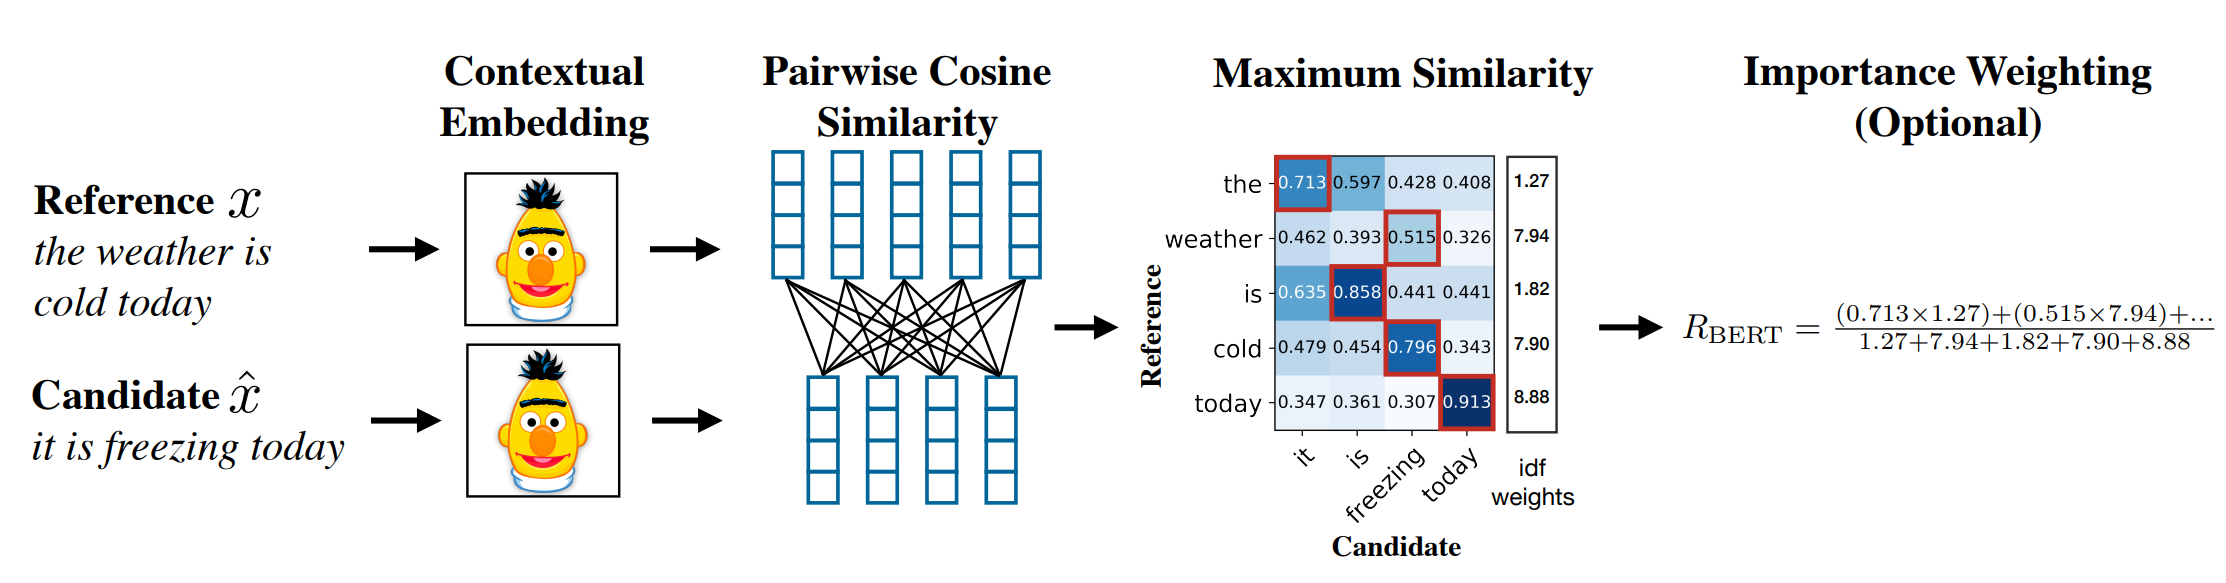
\includegraphics[width=\textwidth]{../images/image003}
					\caption{شبیه سازی نحوه کارکرد \lr{BERTSCORE}}
					\label{BERTSCORE}
				\end{figure}
				
				
				یکی از ویژگی‌های کلیدی \lr{BERTSCORE}، توانایی آن در ارزیابی دقیق جملاتی است که به لحاظ ساختاری متفاوت اما از نظر معنایی مشابه هستند. برای مثال، در جمله مرجع \lr{"the weather is cold today"} و جمله کاندید \lr{"it is freezing today"}، کلماتی مانند \lr{"cold"} و \lr{"freezing"} به درستی تطابق داده می‌شوند، زیرا جاسازی‌های زمینه‌ای معنای مشابه آن‌ها را ثبت کرده‌اند. چنین قابلیتی در معیارهایی مانند \lr{BLEU} و \lr{ROUGE} وجود ندارد، زیرا این معیارها تنها به تطابق دقیق کلمات تکیه دارند. \cite{zhang_bertscore_2020}
			
				
			
			\subsection{\lr{Hallucination}}
				مدل \lr{HHEM-2.1-Open} که توسط \lr{Vectara} توسعه یافته است، برای شناسایی و ارزیابی توهمات در مدل‌های زبانی بزرگ طراحی شده است. این مدل به‌طور ویژه برای کاربردهایی مانند تولید متن بر اساس بازیابی اطلاعات مفید است، جایی که مدل‌های زبانی باید خلاصه‌هایی سازگار با اطلاعات منبع ارائه دهند. \lr{HHEM-2.1-Open} با قابلیت ارزیابی دقیق و سریع، می‌تواند میزان نزدیکی متون تولیدشده را با متون اصلی مقایسه و نرخ توهم مدل را اندازه‌گیری کند. نسخه جدید این مدل نسبت به نسخه‌های قبلی و حتی مدل‌های پیشرفته‌ای مانند \lr{GPT-3.5-Turbo} و \lr{GPT-4} عملکرد بهتری ارائه می‌دهد. یکی از مزایای کلیدی این مدل کارایی بالای آن است؛ به‌طوری که بر روی سخت‌افزارهای معمولی اجرا شده و با استفاده از حافظه کمی (کمتر از ۶۰۰ مگابایت)، ورودی‌هایی با ۲۰۰۰ توکن را در حدود ۱.۵ ثانیه پردازش می‌کند. \lr{HHEM-2.1-Open} به‌عنوان یک مدل طبقه‌بندی توالی، ورودی‌ها را پردازش کرده و امتیازی بین ۰ تا ۱ ارائه می‌دهد؛ عدد ۰ نشان‌دهنده عدم توهم و عدد ۱ نشان‌دهنده توهم کامل است. این مدل نه تنها در تشخیص توهمات تولید متن کاربرد دارد. روش استفاده از این مدل را در جدول \ref{Hallucination} مشاهده می‌کنید. \cite{hhem-2.1-open}
				\begin{table}[ht]
					\centering
					\caption{محاسبه نرخ توهم (\lr{Hallucination}) دو متن.}
					\begin{latin}
						\begin{adjustbox}{width=\textwidth}
						\begin{tabular}{|p{5cm}|p{5cm}|p{2cm}|}
							\hline
							\textbf{Input 1} &
							\textbf{Input 2} &
							\textbf{Output (Result)} \\ \hline
							The capital of France is Berlin. &
							The capital of France is Paris. &
							0.0111 \\ \hline
							I am in California &
							I am in United States. &
							0.6474 \\ \hline
							I am in United States &
							I am in California. &
							0.1290 \\ \hline
							A person on a horse jumps over a broken down airplane. &
							A person is outdoors, on a horse. &
							0.8969 \\ \hline
							A boy is jumping on skateboard in the middle of a red bridge. &
							The boy skates down the sidewalk on a red bridge &
							0.1846 \\ \hline
							A man with blond-hair, and a brown shirt drinking out of a public water fountain. &
							A blond man wearing a brown shirt is reading a book. &
							0.0050 \\ \hline
							Mark Wahlberg was a fan of Manny. &
							Manny was a fan of Mark Wahlberg. &
							0.0543 \\ \hline
						\end{tabular}
						\end{adjustbox}
					\end{latin}
					\label{Hallucination}
				\end{table}

		
	\chapter{ارتقای دانش داخلی}
	
		\section{کتابخوانه‌ها}
		
			\subsection{\lr{HuggingFace Transformers}}
				
				کتابخانه \lr{HuggingFace Transformers} یکی از محبوب‌ترین ابزارهای متن‌باز در حوزه یادگیری ماشین و پردازش زبان طبیعی (NLP) است که امکاناتی جامع برای استفاده و آموزش از مدل‌ها فراهم می‌کند.
				در تنظیم دقیق مدل‌های زبانی پکیج \lr{Transformers} به عنوان یک پکیج پایه استفاده می‌شود.
			
			\subsection{\lr{Llama Factory}}
				
				\lr{LLaMA-Factory}
				یک پکیج متن‌باز است که برای مدیریت، تنظیم دقیق، و بهینه‌سازی مدل‌های زبان بزرگ طراحی شده است. این ابزار پیشرفته، امکاناتی برای آموزش مدل‌ها با استفاده از روش‌های مدرن مانند \lr{LoRA}\LTRfootnote{Low-Rank Adaptation} فراهم می‌کند که کارایی و استفاده از منابع سخت‌افزاری را بهبود می‌بخشد. \lr{LLaMA-Factory} قابلیت مدیریت فرآیندهای پیچیده‌ای مانند تولید مبتنی بر بازیابی\LTRfootnote{RAG} و استفاده ترکیبی از ابزارها در چندین مرحله را ارائه می‌دهد، که این ویژگی‌ها برای حل مسائل چالش‌برانگیز و چندمرحله‌ای کاربردی هستند. این پکیج با ادغام کامل با \lr{PyTorch}، امکاناتی برای توزیع محاسبات و مدیریت حافظه در آموزش مدل‌های بزرگ فراهم می‌کند، که برای کاربرانی با منابع سخت‌افزاری محدود نیز مفید است. همچنین، ابزارهایی برای پیش‌پردازش داده، مدیریت توکنایزرها، و ارزیابی مدل‌ها ارائه می‌دهد که فرآیند آماده‌سازی و بهبود مدل را تسریع می‌بخشند. \cite{zheng2024llamafactory}
			
			\subsection{\lr{Axolotl}}
			
				پکیج \lr{Axolotl} یک ابزار قدرتمند و انعطاف‌پذیر برای تنظیم دقیق مدل‌های زبان بزرگ با تمرکز بر سادگی، مقیاس‌پذیری، و سفارشی‌سازی است. این پکیج به ویژه برای کار با مدل‌های مبتنی بر فریم‌ورک‌های \lr{Hugging Face Transformers} طراحی شده و از روش‌های مدرن مانند LoRA\LTRfootnote{Low-Rank Adaptation} و \lr{QLoRA}\LTRfootnote{Quantized LoRA} پشتیبانی می‌کند که به کاربران امکان می‌دهد مدل‌های بزرگ را با استفاده از منابع سخت‌افزاری محدود آموزش دهند. \lr{Axolotl} با ارائه قابلیت‌هایی مانند مدیریت داده، پیش‌پردازش، و تنظیمات سفارشی برای مدل‌ها، امکان اجرای فرآیندهای پیچیده تنظیم دقیق را بدون نیاز به کدنویسی‌های سنگین فراهم می‌کند. این پکیج همچنین ابزارهایی برای ارزیابی مدل‌ها و تحلیل نتایج ارائه می‌دهد و از \lr{distributed scaling} برای اجرای مدل‌ها در محیط‌های مختلف پشتیبانی می‌کند.
			
			\subsection{\lr{Torch XLA}}
				
				تنظیم دقیق مدل‌ها با استفاده از \lr{Torch XLA} شامل استفاده از شتاب‌دهنده‌های سخت‌افزاری مانند \lr{TPU}\LTRfootnote{Tensor Processing Units} برای بهبود کارایی و سرعت در فرآیند آموزش مدل‌های یادگیری عمیق است. این روش از قدرت بالای محاسبات موازی در \lr{TPU}ها بهره می‌گیرد و با استفاده از XLA\LTRfootnote{Accelerated Linear Algebra}، محاسبات سنگین را بهینه‌سازی و به سرعت اجرا می‌کند. ابتدا مدل و داده‌ها به دستگاه‌های \lr{TPU} منتقل می‌شوند، جایی که توزیع داده‌ها میان هسته‌های متعدد \lr{TPU} برای آموزش موازی انجام می‌گیرد. \lr{Torch XLA }فرآیند همگام‌سازی بین گره‌های توزیع‌شده را مدیریت می‌کند و از تأخیرهای ارتباطی جلوگیری می‌کند. یکی از ویژگی‌های کلیدی این روش، پشتیبانی از \lr{Mixed Precision Training} است که با استفاده از داده‌های \lr{float16} به جای \lr{float32}، حافظه کمتری مصرف می‌کند و سرعت محاسبات را افزایش می‌دهد. این روش با فراهم کردن ابزارهایی برای پروفایلینگ و دیباگینگ، امکان بهینه‌سازی مدل‌ها را ساده می‌کند و برای تنظیم دقیق مدل‌های بزرگ، به ویژه در کاربردهایی مانند پردازش زبان طبیعی ایده‌آل است.
				
				این پکیج در \lr{GitHug} به آدرس \lr{\textbf{https://github.com/axolotl-ai-cloud/axolotl}} موجود است.
			
			\subsection{\lr{NVIDIA NeMo}}
			
				\lr{NVIDIA NeMo}
				یک ابزار قدرتمند و انعطاف‌پذیر برای توسعه مدل‌های زبانی بزرگ و پیچیده است که به محققان و توسعه‌دهندگان اجازه می‌دهد تا به سرعت و به صورت کارآمد مدل‌های سفارشی خود را برای طیف گسترده‌ای از وظایف ایجاد کنند. این چارچوب با ارائه مجموعه‌ای غنی از مدل‌های از پیش آموزش دیده، ابزارهای آماده‌سازی داده و تکنیک‌های بهینه‌سازی، فرآیند توسعه مدل را تسهیل می‌کند. با استفاده از \lr{NeMo}، توسعه‌دهندگان می‌توانند به سرعت مدل‌های زبانی را برای وظایفی مانند تولید متن، ترجمه ماشینی، خلاصه‌سازی متن و تشخیص گفتار آموزش دهند. علاوه بر این، \lr{NeMo} با سخت‌افزارهای قدرتمند \lr{NVIDIA} به خوبی یکپارچه شده است و به این ترتیب به توسعه‌دهندگان اجازه می‌دهد تا از حداکثر توان محاسباتی برای آموزش و استنتاج مدل‌های خود استفاده کنند. به طور کلی، \lr{NeMo} یک ابزار ارزشمند برای توسعه مدل‌های زبانی پیشرفته و کاربردی است.
				
				این پکیج در \lr{GitHug} به آدرس \lr{\textbf{https://github.com/NVIDIA/NeMo}} موجود است.
				
			\subsection{\lr{Xtunner}}
			
				پکیج \lr{XTuner} که در مخزن \lr{GitHub} به آدرس \lr{\textbf{https://github.com/InternLM/xtuner/}} ارائه شده است، ابزاری پیشرفته برای تنظیم دقیق مدل‌های زبان بزرگ با تأکید بر بهینه‌سازی و کاهش هزینه‌های محاسباتی است. این پکیج با پشتیبانی از روش‌های مدرن مانند \lr{LoRA} و \lr{Prefix Tuning}، امکان سفارشی‌سازی مدل‌های پیش‌آموزش‌دیده را برای وظایف خاص فراهم می‌کند. \lr{XTuner} برای ادغام با مدل‌ها و ابزارهای موجود در \lr{Hugging Face Transformers} طراحی شده است. از ویژگی‌های بارز این پکیج می‌توان به انعطاف‌پذیری بالا در تنظیمات، پشتیبانی از آموزش توزیع‌شده، و سازگاری با منابع سخت‌افزاری محدود اشاره کرد. همچنین، \lr{XTuner} ابزارهای پیشرفته‌ای برای مدیریت داده، تنظیم‌های دقیق پارامتر‌ها، و ارزیابی عملکرد مدل‌ها ارائه می‌دهد. این پکیج با استفاده از الگوریتم‌های بهینه‌سازی و معماری‌های کارآمد، امکان کاهش تعداد پارامترهای آموزش‌دیده و حفظ کیفیت مدل را فراهم می‌کند. \cite{2023xtuner}
			
			\subsection{\lr{Unslot}} \label{Unslot}
			
				این پلتفرم با هدف تسریع و ساده‌سازی فرآیندهای مرتبط با مدل‌های زبان بزرگ طراحی شده است و امکاناتی برای تنظیم دقیق، استقرار، و مدیریت این مدل‌ها فراهم می‌کند. \lr{Unsloth} کاربران را قادر می‌سازد تا بدون نیاز به دانش عمیق، مدل‌های از پیش آموزش‌دیده را برای وظایف خاص خود بهینه‌سازی کنند. این مستندات شامل توضیحات دقیقی درباره تنظیمات فنی، ادغام \lr{API}، و روش‌های کار با ابزارهایی مانند \lr{LoRA} برای کاهش هزینه‌های محاسباتی و مصرف منابع است. همچنین، \lr{Unsloth} از ارزیابی مدل‌ها با متریک‌های استاندارد و نظارت بر عملکرد در طول زمان پشتیبانی می‌کند. مستندات \lr{Unsloth} همچنین شامل راهنماهایی برای رفع اشکال و بهترین شیوه‌ها برای بهره‌وری بیشتر در استفاده از مدل‌های هوش مصنوعی است.
				
			مستندات Unsloth AI در آدرس docs.unsloth.ai قرار دارد، راهنمای جامعی برای استفاده از پلتفرم Unsloth ارائه می‌دهد. 
			
			در این پروژه از این پکیج استفاده می‌کنیم چون علاوه بر سادگی در استفاده تضمین می‌کند در بدترین حالت آموزش مدل با سرعت دو برابر انجام شود و از سوی دیگر قابلیت \lr{Quantization} در ابعاد مختلف و ایجاد خروجی قابل اجرا در ابزار \lr{Ollama} را یکجا دارد.
		
		\section{\lr{Supervised Fine-Tuning}}
			
			\subsection{روش‌ها}
			
				\begin{itemize}
					
					\item {\large \lr{LoRA}}
						
						\lr{LoRA}\LTRfootnote{Low-Rank Adaptation}
						روشی نوآورانه برای تطبیق مدل‌های زبانی پیش‌تربیت‌شده بزرگ به وظایف پایین‌دستی است. این روش با کاهش تعداد پارامترهای قابل تنظیم، باعث بهبود کارایی محاسباتی و حافظه شده و در عین حال کیفیت مدل را حفظ می‌کند. ایده اصلی \lr{LoRA} این است که به‌جای به‌روزرسانی مستقیم تمامی وزن‌های مدل، تغییرات وزن‌ها را در قالب ماتریس‌هایی با رتبه پایین (\lr{$\Delta W$}) مدل‌سازی و بهینه‌سازی کند.
						
						در \lr{LoRA}، فرض بر این است که تغییرات مورد نیاز در وزن‌های مدل (\lr{$\Delta W$}) برای تطبیق با یک وظیفه پایین‌دستی، در یک زیرفضای کوچک‌تر نسبت به وزن‌های اصلی قرار دارد. برای پیاده‌سازی این ایده، به‌روزرسانی وزن‌ها به‌صورت زیر مدل‌سازی می‌شود:
						​
						\begin{center}
							\lr{$B A +‌ W_0 = \Delta W + W_0$}
						\end{center}
						
						که در آن:
						
						\begin{itemize}
							
							\item \lr{$W_0$}:
							ماتریس وزن پیش‌تربیت‌شده و ثابت مدل است.
							
							
							\item \lr{$A$} و \lr{$B$}:
							ماتریس‌های قابل تنظیم با ابعاد کوچک‌تر (رتبه پایین) هستند، به‌طوری‌که
							$B \in \mathbb{R}^{d \times r}, \quad A \in \mathbb{R}^{r \times k}, \quad r \ll \min(d, k)$
							
							\item \lr{$r$}:
							رتبه \lr{LoRA}، که به‌طور قابل توجهی کوچک‌تر از ابعاد وزن اصلی انتخاب می‌شود.
							
						\end{itemize}
						
						به این ترتیب، به‌جای بهینه‌سازی مستقیم وزن‌های 
						\lr{$W_0$}
						، تنها ماتریس‌های 
						\lr{$A$} و \lr{$B$}
						که تغییرات وزن را مدل‌سازی می‌کنند، آموزش داده می‌شوند. این امر باعث کاهش تعداد پارامترهای قابل تنظیم می‌شود و حافظه و زمان محاسباتی مورد نیاز را کاهش می‌دهد. (تصویر \ref{LoRA})
						
										
						\begin{figure}[ht]
							\centering
							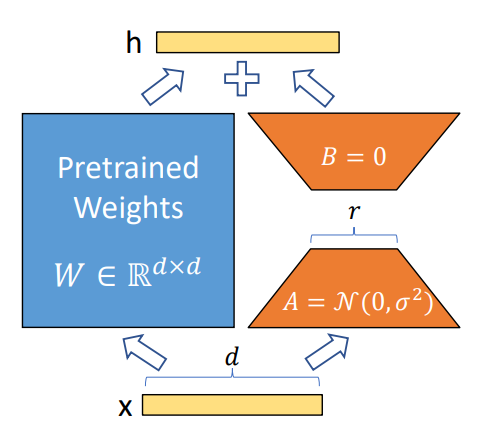
\includegraphics[width=0.5\textwidth]{../images/image006}
							\caption{عملکرد \lr{LoRA}}
							\label{LoRA}
						\end{figure}
						
						
						در فرآیند آموزش، وزن‌های پیش‌تربیت‌شده
						\lr{$W_0$}
						ثابت نگه داشته می‌شوند. ماتریس‌های
						\lr{$A$} و \lr{$B$}
						با مقداردهی اولیه مناسب (صفر برای 
						\lr{$B$}
						و مقادیر تصادفی برای 
						\lr{$B$}
						بهینه‌سازی می‌شوند. برای بهینه‌سازی تغییرات وزن (
						\lr{$B A = \Delta W$}
						)، یک ضریب مقیاس‌بندی (
						\lr{$\frac{\alpha}{r}$}
						) نیز اعمال می‌شود که مقدار آن به‌طور پیش‌فرض متناسب با رتبه \lr{LoRA} تنظیم می‌شود. این طراحی باعث می‌شود که تغییرات اولیه کوچک باشند و روند بهینه‌سازی پایدارتر شود.
						
						هنگام استنتاج، ماتریس‌های به‌روزرسانی‌شده 
						\lr{$A$} و \lr{$B$}
						می‌توانند به صورت صریح با وزن‌های اصلی 
						\lr{$W_0$}
						ترکیب شوند تا وزن نهایی 
						\lr{$\Delta W +‌W_0 = W$}
						محاسبه شود. این فرآیند باعث می‌شود که مدل بتواند بدون هیچ تأخیری در زمان استنتاج، مشابه مدل‌های تنظیم‌شده کامل عمل کند. این ویژگی \lr{LoRA} را برای استفاده در کاربردهای عملی، به‌ویژه در محیط‌هایی با محدودیت سخت‌افزاری، بسیار ارزشمند می‌کند.
						
						\lr{LoRA}
						چندین مزیت کلیدی دارد. نخست، این روش تعداد پارامترهای قابل تنظیم را به طور چشمگیری کاهش می‌دهد، به‌طوری‌که در مدل‌های بسیار بزرگ مانند \lr{GPT-3}، تنها 0.01 درصد از کل پارامترها نیاز به تنظیم دارند. دوم، این روش حافظه و سخت‌افزار مورد نیاز را کاهش می‌دهد؛ زیرا نیازی به محاسبه گرادیان برای تمام وزن‌ها وجود ندارد. علاوه بر این، \lr{LoRA} تأخیری در زمان استنتاج ایجاد نمی‌کند، چرا که وزن‌های به‌روزرسانی‌شده می‌توانند مستقیماً با وزن‌های اصلی ادغام شوند. همچنین، قابلیت جابه‌جایی سریع بین وظایف مختلف، از دیگر مزایای این روش است.
						
						با وجود مزایای \lr{LoRA}، چالش‌هایی نیز وجود دارد. برای مثال، در مواردی که نیاز به پردازش هم‌زمان ورودی‌های چندوظیفه‌ای وجود دارد، اجرای \lr{LoRA} ممکن است دشوار باشد، مگر اینکه وزن‌ها به صورت پویا مدیریت شوند. همچنین، اگرچه \lr{LoRA} عملکرد بالایی با رتبه‌های کوچک ارائه می‌دهد، انتخاب رتبه مناسب \lr{$r$} برای برخی وظایف ممکن است نیازمند آزمون و خطای بیشتری باشد. \cite{hu_lora_2021}
					
					\item {\large \lr{QLoRA}}
					
					\lr{QLORA}
					به معرفی روشی نوآورانه برای تنظیم دقیق مدل‌های زبان بزرگمی‌پردازد که هدف اصلی آن کاهش مصرف حافظه و منابع سخت‌افزاری است. این روش با استفاده از کوانت‌سازی 4 بیتی و \lr{LoRA}، امکان تنظیم دقیق مدل‌هایی با اندازه‌های بسیار بزرگ (تا 65 میلیارد پارامتر) را روی سخت‌افزارهای مصرفی و حرفه‌ای فراهم می‌کند. روش \lr{QLORA} بدون کاهش عملکرد، مصرف حافظه را به‌طور قابل‌توجهی کاهش می‌دهد و با استفاده از تکنیک‌هایی مانند \lr{NF4}\LTRfootnote{NormalFloat 4-bit}، کوانت‌سازی دوگانه و بهینه‌سازهای صفحه‌بندی‌شده، کارایی خود را بهبود می‌بخشد. در تصویر \ref{QLoRA} تفاوت \lr{Full Fine-tuning} با روش‌های \lr{LoRA} و \lr{QLoRA} را می‌بینیم که در \lr{QLoRA} از \lr{paged optimizer} استفاده شده است تا حافظه بهتر مدیریت شود. 
					
					\begin{figure}[ht]
						\centering
						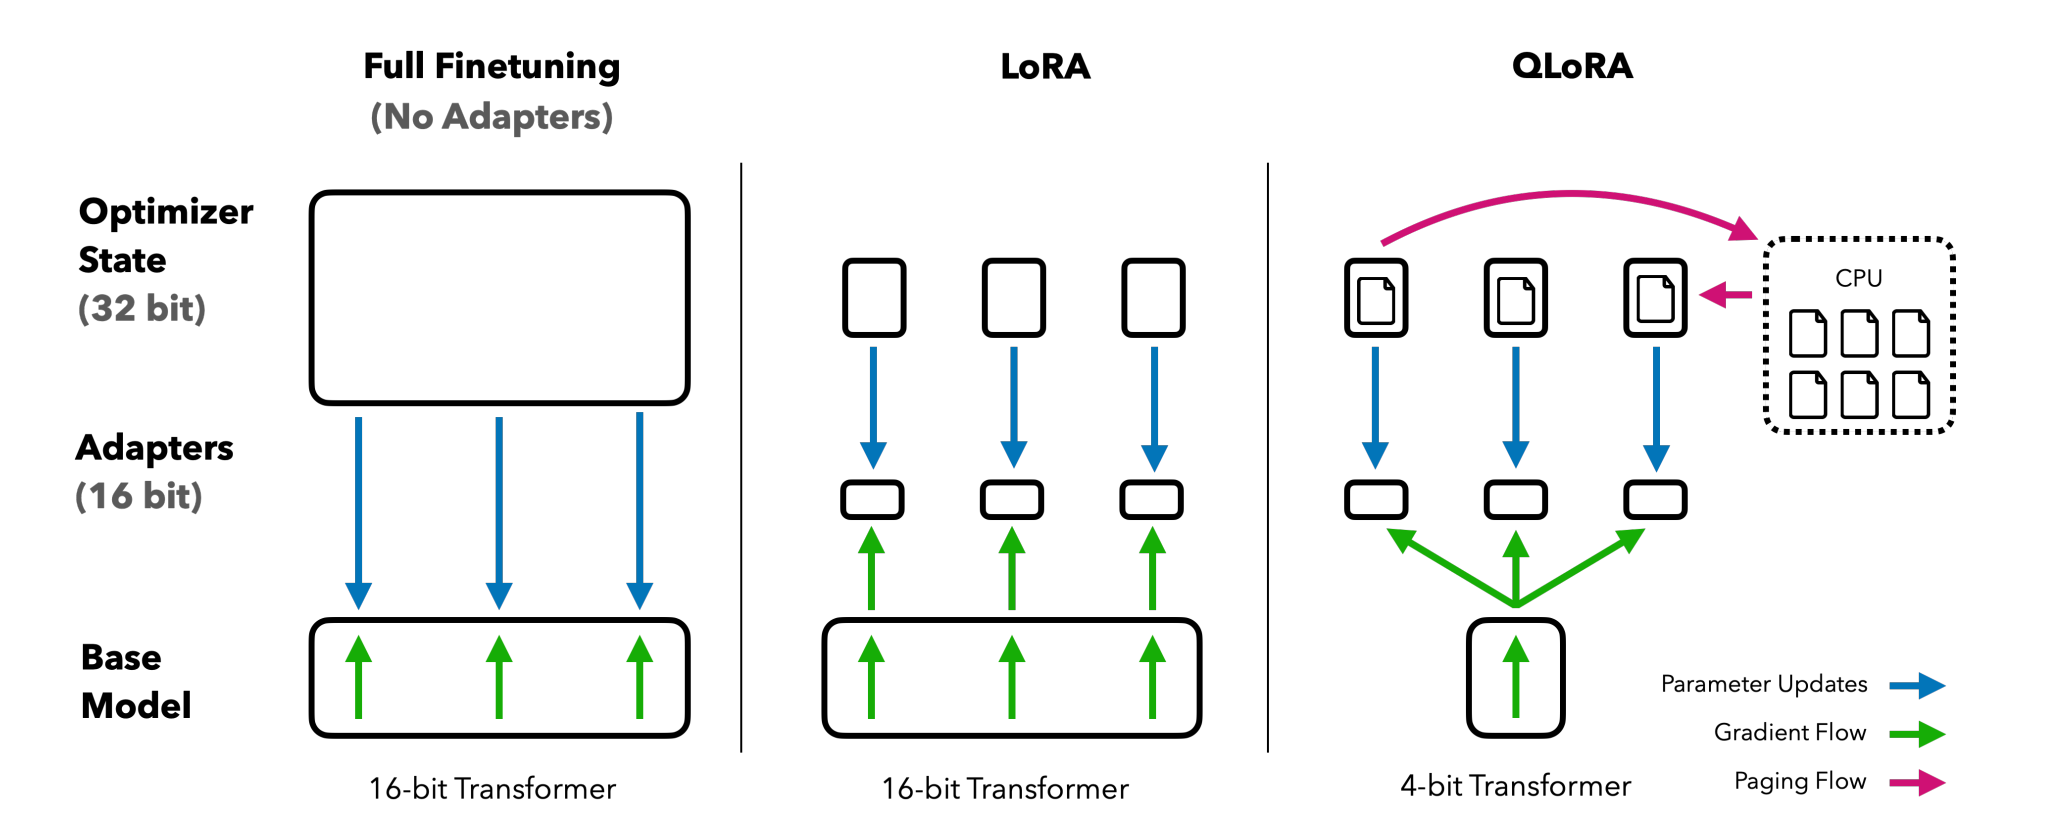
\includegraphics[width=\textwidth]{../images/image007}
						\caption{مقایسه \lr{Full Fine-tuning} با روش‌های \lr{LoRA} و \lr{QLoRA}}
						\label{QLoRA}
					\end{figure}
						
						نتایج این مقاله نشان می‌دهد که \lr{QLORA} در بنچمارک‌های استاندارد مانند \lr{MMLU} و \lr{Vicuna} عملکردی معادل یا بهتر از تنظیم دقیق کامل 16 بیتی دارد. این روش، داده‌های ذخیره‌سازی 4 بیتی را به نوع داده‌های محاسباتی 16 بیتی تبدیل می‌کند تا دقت محاسبات حفظ شود و گرادیان‌ها فقط برای پارامترهای \lr{LoRA} محاسبه شوند. بررسی کیفی نشان داد که مدل تنظیم‌شده با \lr{QLORA} در پاسخ به سؤالات عمومی بسیار دقیق است، اما در مواجهه با سؤالات پیچیده‌تر ممکن است پاسخ‌های اشتباه تولید کند.
						
						از محدودیت‌های این روش، عدم ارزیابی در مقیاس‌های بسیار بزرگ‌تر و بررسی‌های محدود روی سوگیری‌های اجتماعی است. با این وجود، \lr{QLORA} ابزار مهمی برای افزایش دسترسی به تنظیم دقیق مدل‌های زبانی است، به‌ویژه برای پژوهشگرانی که منابع محدودی دارند. همچنین، این روش می‌تواند تنظیم دقیق مدل‌ها را بر روی دستگاه‌هایی با ‌منابع محدود امکان‌پذیر کند. \cite{dettmers_qlora_2023}
					
					\item {\large \lr{DLoRA}}
					
						مدل‌های زبانی بزرگ به دلیل قابلیت‌های خود در انجام وظایف پیچیده پردازش زبان طبیعی (مانند ترجمه، خلاصه‌سازی و تولید متن) به ابزارهای کلیدی در حوزه هوش مصنوعی تبدیل شده‌اند. با این حال، بهینه‌سازی این مدل‌ها برای داده‌ها و وظایف خاص کاربران، نیازمند تنظیم دقیق پارامترها است. این فرآیند با چالش‌هایی نظیر هزینه‌های بالای محاسباتی، نگرانی‌های حریم خصوصی، و مقیاس‌پذیری مواجه است.
						
						برای حل این مشکلات، مقاله راهکاری به نام \lr{DLoRA} پیشنهاد می‌دهد که یک چارچوب توزیع‌شده برای تنظیم دقیق پارامترهاست. این چارچوب عملیات تنظیم دقیق را میان سرورهای ابری و دستگاه‌های کاربران توزیع می‌کند. داده‌های کاربران به صورت محلی در دستگاه‌های آن‌ها پردازش شده و تنها اطلاعات غیرحساس، مانند نتایج \lr{Embedding} به سرور ارسال می‌شود. این رویکرد ضمن کاهش خطرات حریم خصوصی، امکان تنظیم دقیق مدل‌ها را حتی در دستگاه‌هایی با منابع محدود فراهم می‌کند. (تصویر \ref{DLoRA})
						
						\begin{figure}[ht]
							\centering
							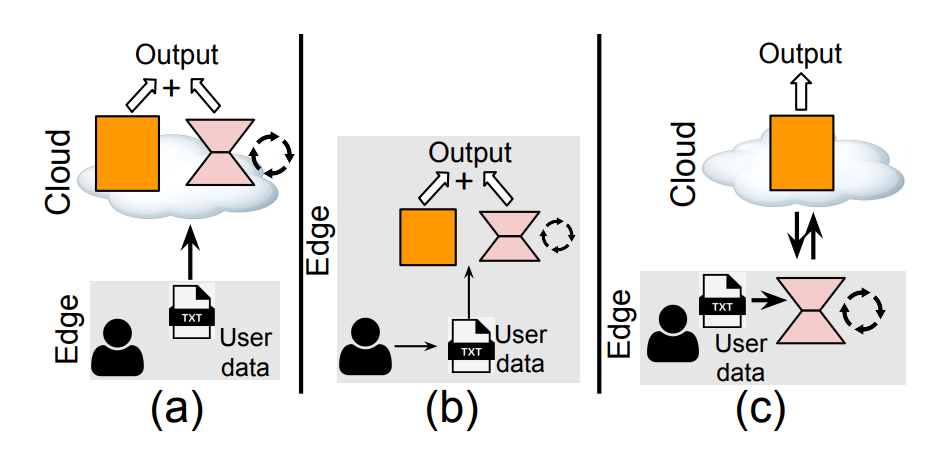
\includegraphics[width=0.6\textwidth]{../images/image008}
							\caption{(\lr{a}) راهکار فقط ابری.
								(\lr{b}) راهکار فقط لبه‌ای.
								(\lr{c}) طرح \lr{DLoRA}. پارامترهای ثابت و قابل یادگیری به ترتیب با رنگ نارنجی و قرمز نشان داده شده‌اند.}
							\label{DLoRA}
						\end{figure}
						
						یکی از نوآوری‌های اصلی مقاله، الگوریتم \lr{KR}\LTRfootnote{Kill and Revive} است. این الگوریتم دو مکانیسم اصلی را معرفی می‌کند: در مرحله اول، ماژول‌هایی از مدل که تغییرات ناچیزی در طی فرآیند تنظیم دقیق دارند شناسایی و به حالت غیرفعال درمی‌آیند تا از بار محاسباتی کاسته شود. این فرآیند که به نام \lr{Early-Kill} شناخته می‌شود، باعث کاهش هزینه‌های ارتباطی و محاسباتی می‌شود. در مرحله دوم، الگوریتم به صورت پویا ماژول‌هایی را که در مراحل بعدی ممکن است اهمیت پیدا کنند، دوباره فعال می‌کند. این مرحله با نام \lr{Revival} شناخته می‌شود و دقت کلی مدل را حفظ کرده یا حتی بهبود می‌بخشد.
						
						ارزیابی‌ها نشان داده‌اند که \lr{DLoRA} و الگوریتم \lr{KR} نه‌تنها هزینه‌های محاسباتی را به میزان 82٪ و حجم ارتباطات را به میزان 87.5٪ کاهش می‌دهند، بلکه دقت مدل را نیز در بسیاری از وظایف حفظ یا بهبود می‌بخشند. این نتایج در مقایسه با روش‌های پایه مانند \lr{FT}\LTRfootnote{Fully-Tune} و روش‌های فشرده‌سازی مدل‌ها مانند \lr{SparseGPT} و \lr{Wanda}، عملکرد برتری را نشان می‌دهد.
						
						\lr{DLoRA}
						همچنین قابلیت مقیاس‌پذیری بالایی دارد و می‌تواند با افزایش تعداد کاربران یا داده‌ها به راحتی سازگار شود. با توجه به اینکه داده‌های خام کاربران در دستگاه‌های آن‌ها باقی می‌ماند، این چارچوب نگرانی‌های مرتبط با حریم خصوصی را برطرف کرده و امنیت داده‌ها را تضمین می‌کند.
						
						در مجموع، مقاله نشان می‌دهد که \lr{DLoRA} می‌تواند به عنوان راهکاری مؤثر و کارآمد برای تنظیم دقیق مدل‌های زبانی بزرگ در محیط‌های توزیع‌شده استفاده شود. این چارچوب با کاهش هزینه‌ها، حفظ دقت، و رفع نگرانی‌های حریم خصوصی، گامی مهم در جهت کاربرد عملی مدل‌های زبانی بزرگ در مقیاس وسیع است. \cite{gao_dlora_2024}
					
					\item {\large روش‌های دیگر}
					
						روش‌های دیگری نیز مانند روش‌های:
						
						\begin{itemize}
							
							\item \lr{LoHa}
							
							\item \lr{LoKr}
							
							\item \lr{adaLoRa}
							
							\item \lr{Prefix-tuning}
							
							\item \lr{OLoRA}
							
							\item \lr{LoftD}
							
							\item \lr{PiSSA}
							
							\item و روش‌های دیگری
							
						\end{itemize}
						
						وجود دارند ولی ما در این پروژه آنها را بررسی نمی‌کنیم.
					
				\end{itemize}
					
			
			\subsection{گزارش \lr{Supervised Fine-Tuning} مدل}
			
				شامل کانفیگ‌ها، دیتاست‌ها، نمودارهای loss و ارزیابی
				
			
		\section{\lr{Alignment}}
			\subsection{\lr{RLHF}}
			
				روش ارائه‌شده در مقاله برای تنظیم دقیق مدل‌های زبانی با استفاده از یادگیری تقویتی مبتنی بر بازخورد انسانی (\lr{RLHF}) شامل سه مرحله اصلی است که به صورت متوالی اجرا می‌شود. این روش با هدف همسوسازی مدل‌های زبانی با نیات انسانی طراحی شده است و از داده‌های جمع‌آوری‌شده توسط برچسب‌گذاران انسانی استفاده می‌کند.
				
				در مرحله اول، داده‌های نمایشی جمع‌آوری می‌شوند. برچسب‌گذاران انسانی خروجی‌های مطلوبی را برای دستورات مختلف ارائه می‌دهند تا رفتار ایده‌آل مدل مشخص شود. سپس مدل \lr{GPT-3} از پیش‌آموزش‌دیده با استفاده از این داده‌ها از طریق یادگیری نظارت‌شده تنظیم دقیق می‌شود. این مرحله به مدل کمک می‌کند تا رفتارهای اولیه‌ای که با نیات انسانی همسو هستند، یاد بگیرد و در خروجی‌های خود اعمال کند.
				
				در مرحله دوم، داده‌های مقایسه‌ای جمع‌آوری می‌شوند. برای هر دستور، مدل چندین خروجی مختلف تولید می‌کند و برچسب‌گذاران انسانی خروجی ترجیحی خود را انتخاب می‌کنند. این مقایسه‌ها به‌عنوان ورودی برای آموزش مدل پاداش استفاده می‌شوند. مدل پاداش یاد می‌گیرد که خروجی‌های ترجیحی انسانی را پیش‌بینی کند و از این اطلاعات برای ارزیابی و بهبود عملکرد مدل استفاده می‌شود.
				
				در مرحله سوم، مدل نظارت‌شده با استفاده از مدل پاداش و الگوریتم \lr{PPO} بهینه‌سازی می‌شود. مدل پاداش به‌عنوان سیگنال ارزیابی خروجی‌ها عمل می‌کند و الگوریتم \lr{PPO} سیاست مدل را برای بهبود پاداش دریافتی تنظیم می‌کند. این مرحله به مدل امکان می‌دهد تا در محیط واقعی به‌صورت تقویتی یاد بگیرد و خروجی‌های خود را بهبود بخشد.
				
				این سه مرحله به‌صورت تکراری اجرا می‌شوند تا مدل به تدریج به رفتار مطلوب نزدیک‌تر شود. داده‌های مقایسه‌ای جدید از سیاست‌های بهینه‌شده جمع‌آوری و مدل پاداش بازآموزی می‌شود. این روش ترکیبی از یادگیری نظارت‌شده و یادگیری تقویتی است که هم دقت و هم انعطاف‌پذیری مدل را افزایش می‌دهد و باعث می‌شود خروجی‌های تولیدشده نه‌تنها به دستورات کاربران پاسخ دهند، بلکه با محدودیت‌ها و معیارهای مشخص شده نیز سازگار باشند. \cite{ouyang_training_2022}
					
			\subsection{\lr{DPO}}
			
				\lr{DPO}\LTRfootnote{Direct Preference Optimization}
				یک روش ساده و موثر برای بهینه‌سازی سیاست مدل‌های زبانی با استفاده از ترجیحات انسانی است که برخلاف \lr{RLHF}\LTRfootnote{Reinforcement Learning from Human Feedback}، نیازی به یادگیری تقویتی ندارد. در DPO، فرآیند یادگیری به یک مسئله طبقه‌بندی کاهش می‌یابد، جایی که سیاست مدل مستقیماً برای افزایش احتمال پاسخ‌های ترجیحی و کاهش احتمال پاسخ‌های رد شده آموزش داده می‌شود.
				
				در روش \lr{RLHF}، مدل پاداش به‌طور جداگانه آموزش داده می‌شود تا ترجیحات انسانی را مدل‌سازی کند و سپس با استفاده از یادگیری تقویتی، سیاست مدل زبانی بهینه‌سازی می‌شود. در مقابل، \lr{DPO} با استفاده از یک بازپارامترسازی خاص، تابع زیان را مستقیماً بر اساس سیاست مدل تعریف می‌کند. این بازپارامترسازی به ما اجازه می‌دهد که بدون نیاز به یادگیری صریح یک مدل پاداش یا انجام یادگیری تقویتی پیچیده، سیاست بهینه را استخراج کنیم. مقایسه این دو روش در جدول \ref{DPO_vs_RLHF} و تصویر \ref{DPO_RLHF} انجام شده است. \cite{rafailov_direct_2024}
				
				\begin{figure}[ht]
					\centering
					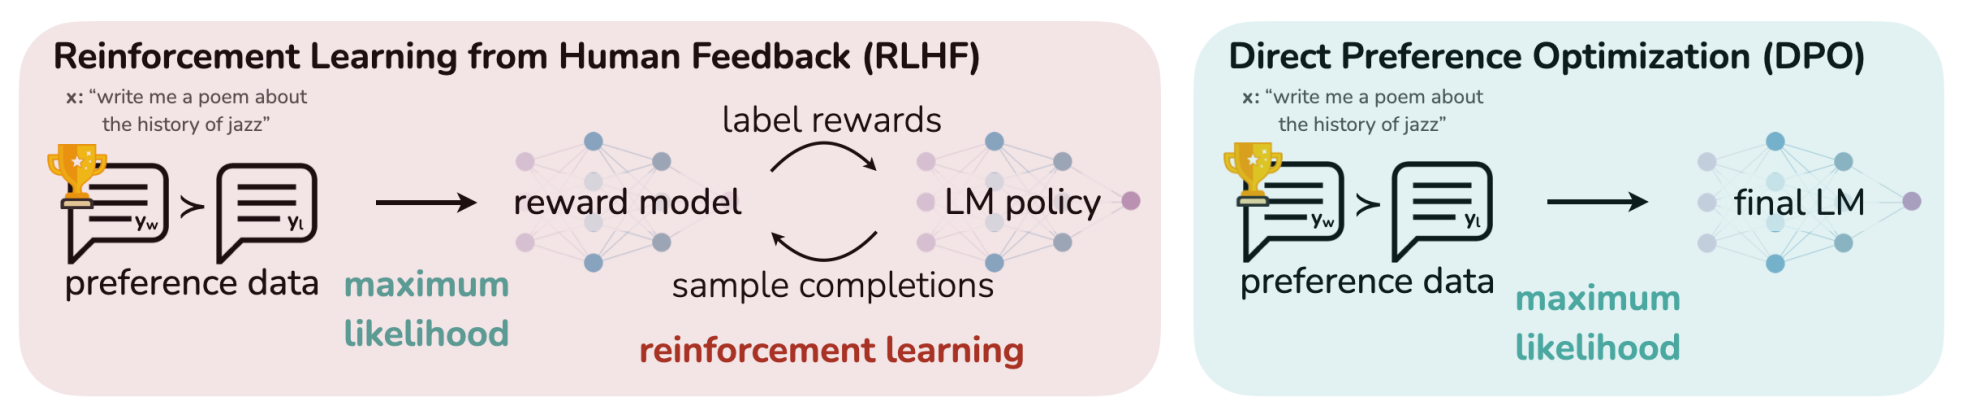
\includegraphics[width=\textwidth]{../images/image009}
					\caption{مقایسه روش \lr{DPO} با \lr{RLHF}}
					\label{DPO_RLHF}
				\end{figure}
				
				مراحل اصلی روش \lr{DPO}:
				\begin{enumerate}
					
					\item {\large نمونه‌برداری و برچسب‌گذاری داده‌ها}:
					جفت‌هایی از پاسخ‌ها 
					​\lr{($y_l, y_w$)}
					برای هر پرامپت 
					\lr{$x$}
					از یک سیاست مرجع (
					\lr{$\pi_{ref}$}
					) نمونه‌برداری می‌شوند. سپس برچسب‌گذاران انسانی پاسخ ترجیحی (
					\lr{$y_w$}
					) و پاسخ رد شده (
					\lr{$y_l$}
					) را مشخص می‌کنند.
					
					\item {\large تعریف تابع زیان \lr{DPO}}:
					تابع زیان بر اساس مدل \lr{Bradley-Terry} برای ترجیحات انسانی تعریف می‌شود. این تابع زیان به صورت زیر است:
					
					\begin{center}
						\lr{$\mathcal{L}_{DPO}(\pi_\theta; \pi_{ref}) = -\mathbb{E}_{(x, y_w, y_l) \sim D} \left[ \log \sigma \left( \beta \log \frac{\pi_\theta(y_w \mid x)}{\pi_{ref}(y_w \mid x)} - \beta \log \frac{\pi_\theta(y_l \mid x)}{\pi_{ref}(y_l \mid x)} \right) \right]$}
					\end{center}
					
					در اینجا:
					
					\begin{itemize}
						
						\item {\large \lr{$\pi_\theta(y \mid x)$}}: سیاست فعلی مدل
						
						\item {\large \lr{$\pi_{ref}(y \mid x)$}}: سیاست مرجع
						
						\item {\large \lr{$\beta$}}:‌ پارامتری که میزان سخت‌گیری محدودیت \lr{KL} را کنترل می‌کند.

					\end{itemize}
					
					\item {\large بهینه‌سازی سیاست مدل}:
					
					مدل زبانی (
					\lr{$\pi_\theta$}
					) برای کمینه‌سازی تابع زیان 
					\lr{$\mathcal{L}_{DPO}$}
					آموزش داده می‌شود. گرادیان این تابع زیان به گونه‌ای عمل می‌کند که احتمال پاسخ‌های ترجیحی 
					\lr{$y_w$}
					​
					را افزایش داده و احتمال پاسخ‌های رد شده 
					\lr{$y_l$}
					را کاهش دهد.
					
				\end{enumerate}
				
				\begin{table}[h!]
					\centering
					\caption{مقایسه روش \lr{DPO} با \lr{RLHF}}
					\begin{adjustbox}{max width=\textwidth}
						\begin{tabular}{|l|p{5.5cm}|p{5.5cm}|}
							\hline
							\textbf{ویژگی} & \lr{DPO} & \lr{RLHF} \\
							\hline
							\textbf{پیچیدگی} & ساده و بدون نیاز به یادگیری تقویتی & پیچیده؛ نیازمند دو مرحله (آموزش مدل پاداش و یادگیری تقویتی) \\
							\hline
							\textbf{نیاز به مدل پاداش} & بدون نیاز به مدل پاداش مجزا؛ تابع پاداش به‌طور ضمنی با سیاست مدل بازنمایی می‌شود & نیاز به یادگیری یک مدل پاداش صریح برای مدل‌سازی ترجیحات انسانی \\
							\hline
							\textbf{تابع زیان} & یک \textit{تابع زیان دوجمله‌ای (\lr{cross-entropy})} ساده & ترکیبی از تابع پاداش و محدودیت KL در یادگیری تقویتی \\
							\hline
							\textbf{پایداری} & پایدار؛ به دلیل عدم نیاز به نمونه‌برداری از مدل حین آموزش & اغلب ناپایدار؛ به دلیل وابستگی به نمونه‌برداری از مدل و محاسبات پیچیده تابع پاداش \\
							\hline
							\textbf{کارایی محاسباتی} & بسیار کارآمد؛ نیازی به محاسبات سنگین یادگیری تقویتی ندارد & هزینه‌بر؛ شامل آموزش چند مدل زبانی و نمونه‌برداری‌های مکرر از مدل در حلقه یادگیری \\
							\hline
							\textbf{انحراف \lr{KL}} & انحراف از سیاست مرجع به‌طور ذاتی در تابع زیان لحاظ شده است & به طور مستقیم از طریق محدودیت \lr{KL} در فرآیند \lr{RLHF} کنترل می‌شود \\
							\hline
							\textbf{کاربرد در عمل} & پیاده‌سازی آسان و سریع، حتی برای مدل‌های بزرگ & بهینه‌سازی پیچیده و نیازمند تنظیم دقیق ابرپارامترها \\
							\hline
							\textbf{عملکرد تجربی} & در آزمایش‌ها عملکردی مشابه یا بهتر از \lr{RLHF} (\lr{PPO}) داشت & عملکرد خوب، اما با هزینه محاسباتی بالا و ناپایداری احتمالی \\
							\hline
						\end{tabular}
					\end{adjustbox}
					\label{DPO_vs_RLHF}
				\end{table}

					
			\subsection{\lr{KTO}}
				
				\lr{KTO}
				یک روش جدید برای هم‌ترازی مدل‌های زبانی بزرگ است که از اصول تئوری چشم‌انداز کاهنمن و تورسکی بهره می‌برد. این روش مستقیماً مطلوبیت انسانی را به جای احتمال ترجیحات یا پاداش‌های مدل‌سازی‌شده بهینه می‌کند. \lr{KTO} از سیگنال دودویی (خوب/بد) به‌جای ترجیحات جفتی یا مدل پاداش استفاده می‌کند و تابع زیان آن برای ادراک انسانی طراحی شده است. مقایسه این روش با دو روش قبل در جدول \ref{KTO_DPO_RLHF} آمده است. \cite{ethayarajh_kto_2024}
				
				ویژگی‌های اصلی \lr{KTO}:
				
					\begin{enumerate}
						
						\item {\large تابع مطلوبیت مبتنی بر تئوری چشم‌انداز}:
						
						مطلوبیت یک خروجی با استفاده از تابع ارزش کاهنمن-تورسکی محاسبه می‌شود که حساسیت به سودها و زیان‌ها را با ضرایب جداگانه (
						\lr{$\lambda_D$}
						و 
						\lr{$\lambda_U$}
						) و پارامتر ریسک‌گریزی (
						\lr{$\beta$}
						) کنترل می‌کند.
						
						\item {\large استفاده از سیگنال دودویی}:
						
						برخلاف روش‌های \lr{DPO} و \lr{RLHF}، \lr{KTO} تنها به بازخورد ساده مطلوب یا نامطلوب نیاز دارد و نیازی به داده‌های پیچیده ترجیحی ندارد.
						
						\item {\large تخمین نقطه مرجع با واگرایی \lr{KL}}:
						
						یک نقطه مرجع 
						\lr{$z_0$}
						برای ارزیابی کیفیت خروجی‌ها تعریف می‌شود که با استفاده از واگرایی KL محاسبه می‌شود و کیفیت نسبی خروجی‌ها را نسبت به مدل مرجع (
						\lr{$\pi_{ref}$}
						) اندازه‌گیری می‌کند.
						
						\item {\large مزیت در داده‌های نامتعادل}:
						
						\lr{KTO}
						می‌تواند حتی با تعداد کمی از داده‌های مطلوب (در مقایسه با داده‌های نامطلوب) عملکرد مطلوبی ارائه دهد.
						
					\end{enumerate}
					
					تابع \lr{loss} \lr{KTO} به شکل زیر تعریف می‌شود:
					
					\begin{center}
						\lr{$L_{KTO}(\pi_\theta, \pi_{ref}) = \mathbb{E}_{x, y \sim D} \left[\lambda_y - v(x, y)\right]$}
					\end{center}
					
					که در آن:
					
					\begin{itemize}
						
						\item {\large \lr{$r_\theta(x, y) = \log \left(\frac{\pi_\theta(y \mid x)}{\pi_{ref}(y \mid x)}\right)$}}:
						نشان‌دهنده کیفیت خروجی \lr{$y$} است.
					
						\item {\large \lr{$v(x, y)$}}:‌
						تابع مطلوبیت که با توجه به خروجی مطلوب یا نامطلوب به صورت زیر تعریف می‌شود:
						\begin{center}
							\lr{$v(x,y) = \begin{cases}
									\lambda_D \cdot \sigma(\beta \cdot (r_{\theta}(x,y) - z_0)) & if: y \sim y_{desirable} \mid x \\
									\lambda_U \cdot \sigma(\beta \cdot (z_0 - r_{\theta}(x,y))) & if: y \sim y_{undesirable} \mid x
								\end{cases}$}
						\end{center}
						
						\item {\large \lr{$z_0$}}:
						نقطه مرجع که کیفیت نسبی خروجی‌ها را تعیین می‌کند و با واگرایی \lr{KL} محاسبه می‌شود:
						\begin{center}
							\lr{$z_0 = KL\left(\pi_\theta(y' \mid x) \, \| \, \pi_{ref}(y' \mid x)\right)$}
						\end{center}
						
					\end{itemize}

					\begin{table}[h!]
						\centering
						\caption{مقایسه روش‌های \lr{KTO}، \lr{DPO} و \lr{RLHF}}
						\begin{adjustbox}{max width=\textwidth}
						\begin{tabular}{|p{3cm}|p{3cm}|p{3cm}|p{3cm}|}
							\hline
							\textbf{ویژگی‌ها} &
							\textbf{\lr{KTO}} &
							\textbf{\lr{DPO}} &
							\textbf{\lr{RLHF}} \\ \hline
							
							\textbf{هدف بهینه‌سازی} &
							مطلوبیت انسانی با استفاده از تابع ارزش کاهنمن-تورسکی &
							احتمال نسبی ترجیحات\LTRfootnote{Preference Likelihood} &
							یادگیری یک مدل پاداش و بهینه‌سازی آن با الگوریتم‌های RL \\ \hline
							
							\textbf{نوع داده موردنیاز} &
							سیگنال دودویی (خوب/بد) &
							داده‌های ترجیحی جفتی (\lr{$y_w \succ y_l$}) &
							داده‌های ترجیحی و مدل پاداش \\ \hline
							
							\textbf{پایداری و سرعت} &
							پایدار و سریع به دلیل استفاده از \lr{Closed-form} توابع &
							نسبتاً پایدار ولی به داده‌های ترجیحی وابسته &
							ناپایدار و کند به دلیل پیچیدگی الگوریتم‌های \lr{RL} \\ \hline
							
							\textbf{تعامل با داده‌های نامتعادل} &
							عملکرد مناسب حتی با داده‌های نامتعادل &
							حساس به تعادل داده‌های ترجیحی &
							حساس به تعادل داده و مستعد افت عملکرد در صورت وجود نویز یا داده‌های محدود \\ \hline
							
							\textbf{کاربرد در مدل‌های اولیه} &
							می‌تواند بدون نیاز به تنظیم دقیق\LTRfootnote{SFT} استفاده شود &
							نیاز به \lr{SFT} برای دستیابی به عملکرد بهتر &
							نیاز شدید به \lr{SFT} برای ایجاد مدل مرجع \\ \hline
							
							\textbf{سادگی پیاده‌سازی} &
							ساده‌تر به دلیل عدم نیاز به یادگیری مدل پاداش و ترجیحات پیچیده &
							نسبتاً ساده، اما نیاز به داده‌های ترجیحی باکیفیت دارد &
							پیچیده به دلیل نیاز به یادگیری مدل پاداش و استفاده از الگوریتم‌های \lr{RL} \\ \hline
							
						\end{tabular}
						\end{adjustbox}
						\label{KTO_DPO_RLHF}
					\end{table}
					
			\subsection{\lr{ORPO}}
			
				روش \lr{ORPO} بر اساس استفاده از نسبت شانس\LTRfootnote{Odds Ratio} برای هم‌ترازی ترجیحات طراحی شده است. این روش برخلاف روش‌های پیچیده مانند \lr{RLHF} یا \lr{DPO}، نیازی به مدل مرجع یا مراحل چندگانه ندارد. \lr{ORPO} تمام فرآیند هم‌ترازی ترجیحات را در یک مرحله انجام می‌دهد و تنها با اضافه‌کردن یک ترم جریمه به تابع خطای معمولی (\lr{Negative Log-Likelihood}) عمل می‌کند. مقایسه آن با روش‌های \lr{DPO} و \lr{RLHF} در جدول \ref{ORPO_DPO_RLHF}	و تصور \ref{ORPO_DPO_RLHF_fig} قرار دارد. \cite{hong_orpo_2024}


				\begin{figure}[ht]
					\centering
					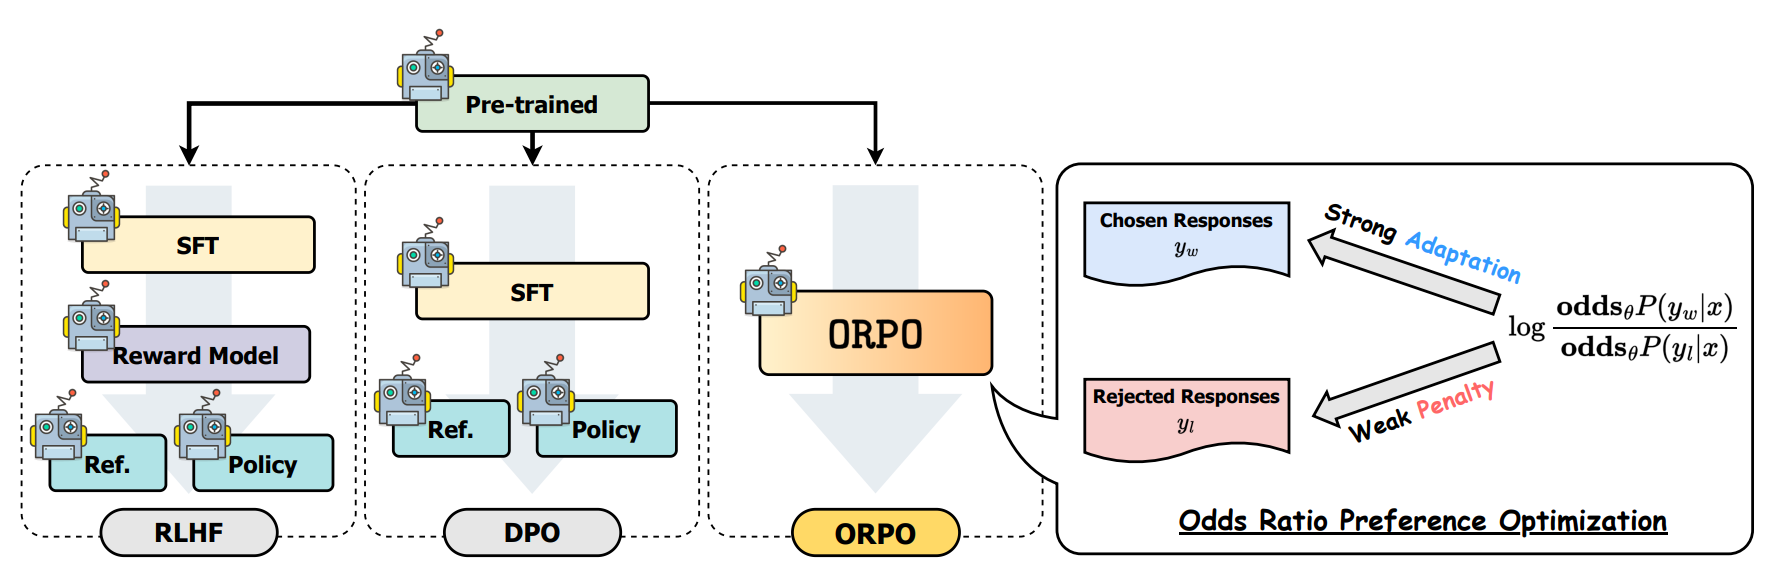
\includegraphics[width=\textwidth]{../images/image010}
					\caption{\lr{ORPO}، \lr{DPO} و \lr{RLHF}}
					\label{ORPO_DPO_RLHF_fig}
				\end{figure}
				
				
				اجزای اصلی \lr{ORPO}:
				
				\begin{enumerate}
					
					\item {\large تابع خطای تنظیم دقیق (\lr{$L_{SFT}$})}:
					
					این تابع به منظور افزایش احتمال تولید پاسخ‌های مطلوب توسط مدل استفاده می‌شود.
					
					\item {\large تابع خطای نسبی نسبت شانس (\lr{$L_{OR}$})}:
					
					این تابع تفاوت بین شانس تولید پاسخ انتخاب‌شده (
					\lr{$y_w$}
					) و پاسخ ردشده (
					\lr{$y_l$}
					) را افزایش می‌دهد. تابع کلی \lr{ORPO} به‌صورت زیر تعریف می‌شود:
					
					\begin{center}
						\lr{$L_{ORPO} = \mathbb{E}_{(x, y_w, y_l)} \left[ L_{SFT} + \lambda \cdot L_{OR} \right]$}
					\end{center}
					در این رابطه:
					
					\begin{center}
						\lr{$L_{OR} = -\log \sigma \left( \log \frac{odds_\theta(y_w|x)}{odds_\theta(y_l|x)} \right)$}
					\end{center}
					
					که در آن 
					\lr{$\sigma$}
					تابع سیگموید است و نسبت شانس (
					\lr{$odds_\theta$}
					) احتمال تولید یک پاسخ مطلوب به یک پاسخ نامطلوب را نشان می‌دهد.
					
				\end{enumerate}
				
				\lr{ORPO}
				به‌صورت پویا شانس تولید پاسخ‌های نامطلوب را کاهش داده و شانس تولید پاسخ‌های مطلوب را تقویت می‌کند. این امر به مدل کمک می‌کند تا به تولید پاسخ‌های هماهنگ با ترجیحات انسانی هدایت شود.
				
				
				مزایای \lr{ORPO}:
				\begin{itemize}
					
					\item {\large حذف نیاز به مدل مرجع}:
					برخلاف روش‌های \lr{DPO} و \lr{RLHF}، \lr{ORPO} تنها با استفاده از مدل تنظیم‌شده\lr{SFT} کار می‌کند و نیازی به مدل مرجع یا مدل پاداش ندارد.
					
					\item {\large کاهش هزینه محاسباتی}:
					این روش تنها به دو \lr{Forward Pass} نیاز دارد، در حالی که روش‌های دیگر مانند \lr{RLHF} و \lr{DPO} به چهار مورد نیازمندند.
					
					\item {\large یکپارچگی مراحل}:
					\lr{ORPO}
					فرآیندهای تنظیم دقیق نظارت‌شده و هم‌ترازی ترجیحات را به‌طور همزمان و یکپارچه انجام می‌دهد، که منجر به سادگی و کارایی بالاتر می‌شود.
					
					
				\end{itemize}
				
				
				\begin{table}[h!]
					\centering
					\caption{جدول مقایسه \lr{ORPO}، \lr{DPO} و \lr{RLHF}}
					\begin{adjustbox}{max width=\textwidth}
					\begin{tabular}{|c|c|c|c|}
						\hline
						\textbf{ویژگی}      & \textbf{\lr{ORPO}}       & \textbf{\lr{DPO}}            & \textbf{\lr{RLHF}}           \\ \hline
						نیاز به مدل مرجع       & ندارد                  & دارد                   & دارد                   \\ \hline
						تعداد مراحل            & یک مرحله              & دو مرحله (\lr{SFT} + \lr{DPO})   & سه مرحله (\lr{SFT} + مدل پاداش + \lr{RLHF}) \\ \hline
						هزینه محاسباتی         & کم                     & متوسط                  & بالا                   \\ \hline
						پیچیدگی تنظیمات        & کم                     & متوسط                  & بالا                   \\ \hline
						مزایا                  & کارایی بالا، کاهش هزینه‌ها & کاهش مراحل نسبت به \lr{RLHF} & تنظیم دقیق‌تر ترجیحات انسانی \\ \hline
						معایب                  & به شانس متکی است & نیاز به مدل مرجع       & پیچیدگی و هزینه بالا   \\ \hline
						کاربرد در مقیاس بالا   & مناسب                 & مناسب                  & محدود به منابع بیشتر   \\ \hline
					\end{tabular}
					\end{adjustbox}
					\label{ORPO_DPO_RLHF}
				\end{table}
				
				
			\subsection{گزارش \lr{Alignment} مدل}
				
				شامل کانفیگ‌ها، دیتاست‌ها، نمودارهای loss و ارزیابی
			
	\chapter{ارتقای دانش خارجی}
	
		\section{فریم‌ورک‌ها}
		
			\subsection{\lr{LangChain}}
				
				کتابخانه \lr{LangChain} مجموعه‌ای از ابزارهای پیشرفته برای ساخت و توسعه برنامه‌های هوش مصنوعی مبتنی بر مدل‌های زبان بزرگ ارائه می‌دهد. این ابزارها در حوزه‌های مختلف از مدیریت پرامپت‌ها تا ادغام داده‌های خارجی و ایجاد زنجیره‌های پردازشی به توسعه‌دهندگان کمک می‌کنند. در ادامه، جزئیات ابزارهای اصلی این کتابخانه آورده شده است:
				
				\begin{enumerate}
					
					\item {\large مدیریت پرامپت‌ها (\lr{Prompt Management})} \par
					این ابزارها به توسعه‌دهندگان امکان می‌دهند پرامپت‌ها را قالب‌بندی، ساختاربندی و مدیریت کنند. ابزارهای مدیریت پرامپت به گونه‌ای طراحی شده‌اند که بتوانید دستوراتی واضح، منسجم و مؤثر برای مدل‌های زبانی ایجاد کنید. این ویژگی به‌خصوص برای ایجاد پاسخ‌های دقیق‌تر و کاهش ابهامات مدل بسیار مفید است.
					
					\item {\large زنجیره‌ها (\lr{Chains})} \par
					زنجیره‌ها هسته اصلی \lr{LangChain} هستند و به شما این امکان را می‌دهند که چندین عملیات یا فراخوانی مدل را به صورت گام‌به‌گام ترکیب کنید. این ابزار برای انجام وظایف پیچیده مانند:
					
					\begin{itemize}
						
						\item سیستم‌های پرسش و پاسخ بر پایه متن
						
						\item ایجاد و تحلیل متن
						
						\item مدیریت فرآیندهای چندمرحله‌ای
						
					\end{itemize}
					
					بسیار مناسب است. به عنوان مثال، زنجیره‌ای می‌تواند شامل بازیابی اطلاعات از یک پایگاه داده، پردازش آن‌ها و سپس تولید پاسخ باشد.
					
					\item {\large بازیاب‌ها (\lr{Retrievers})} \par
					بازیاب‌ها امکان دسترسی به داده‌های خارجی را فراهم می‌کنند. این داده‌ها می‌توانند شامل اسناد، پایگاه‌های داده یا محتوای آنلاین باشند. بازیاب‌ها همچنین قابلیت پردازش داده‌ها را برای آماده‌سازی اطلاعات برای مدل‌های زبانی فراهم می‌کنند.
					
					این ابزار برای ساخت سیستم‌های پرسش و پاسخ مبتنی بر دانش، ادغام داده‌های شرکت و اتصال به منابع داده خارجی استفاده می‌شود.
					
					\item {\large عامل‌ها (\lr{Agents})} \par
					\lr{Agents}
					ابزارهایی هستند که به مدل‌های زبان بزرگ اجازه می‌دهند به صورت پویا و خودکار وظایف مختلف را مدیریت کنند. این ابزارها برخلاف زنجیره‌ها که مسیر از پیش تعریف‌شده دارند، به مدل امکان می‌دهند در زمان اجرا تصمیم بگیرد چه عملیاتی انجام دهد یا از چه ابزاری استفاده کند.
					
					ویژگی‌های کلیدی عامل‌ها:
					
					\begin{itemize}
						
						\item {\large دسترسی به ابزارها}:
						توانایی استفاده از \lr{API}ها، پایگاه‌های داده، موتورهای جستجو و ابزارهای خارجی.
						
						\item {\large تصمیم‌گیری پویا}:
						انتخاب مسیر و ابزار مناسب برای حل مشکلات در لحظه.
						
						\item {\large مدیریت وظایف پیچیده}:
						انجام چند مرحله پردازش یا ادغام اطلاعات از منابع مختلف.
						
					\end{itemize}
					\lr{Agents}
					در وظایفی مانند پرسش و پاسخ پیشرفته، اتوماسیون فرآیندها، و تعامل با خدمات خارجی استفاده می‌شوند. آن‌ها ابزاری انعطاف‌پذیر برای توسعه سیستم‌های هوشمند و پویا هستند.
					
					\item {\large حافظه (\lr{Memory})} \par
					قابلیت حافظه یکی از ویژگی‌های متمایز \lr{LangChain} است که امکان ذخیره و یادآوری تعاملات گذشته را برای مدل فراهم می‌کند. این ابزار برای ساخت ربات‌های چت پیشرفته که باید مکالمات گذشته را به خاطر بسپارند و بر اساس آن‌ها پاسخ دهند، بسیار کاربردی است.
					
					\item {\large ابزارهای اشکال‌زدایی و نظارت (\lr{LangSmith})} \par
					\lr{LangChain}
					ابزاری به نام \lr{LangSmith} ارائه می‌دهد که توسعه‌دهندگان می‌توانند با استفاده از آن عملکرد سیستم‌های خود را نظارت و مشکلات آن‌ها را رفع کنند. این ابزار به صورت گرافیکی اطلاعات مرتبط با زنجیره‌ها و پرامپت‌ها را نمایش می‌دهد و امکان بهینه‌سازی آن‌ها را فراهم می‌کند.
					
					\item {\large ادغام‌پذیری بالا} \par
					\lr{LangChain}
					به گونه‌ای طراحی شده که با ابزارهای مختلف از جمله \lr{Python}، پایگاه‌های داده، و حتی منابع داده خصوصی به‌راحتی ادغام شود.
					
					این ویژگی‌ها \lr{LangChain} را به ابزاری قدرتمند و انعطاف‌پذیر برای ساخت برنامه‌های مبتنی بر هوش مصنوعی تبدیل کرده است.
					
				\end{enumerate}
			
			\subsection{\lr{Llama-Index}}
			
				\lr{LlamaIndex}
				، یک چارچوب منبع‌باز، ابزارهای متنوعی برای مدیریت، ایندکس، و بازیابی داده‌ها ارائه می‌دهد که امکان استفاده بهینه از مدل‌های زبان بزرگ را فراهم می‌کند. در ادامه ابزارها و ویژگی‌های کلیدی این کتابخانه بررسی شده است:
				
				\begin{enumerate}
					
					\item {\large مدیریت داده‌ها (\lr{Data Handling})} \par
					
					\lr{LlamaIndex}
					امکان اتصال و پردازش داده‌های ساختارمند و غیرساختارمند را فراهم می‌کند. این داده‌ها می‌توانند شامل موارد زیر باشند:
					
					\begin{itemize}
						
						\item {\large فایل‌ها}:
						اسناد \lr{PDF}، \lr{Word}، صفحات \lr{Excel}.
						
						\item {\large پایگاه‌های داده}:
						سیستم‌های \lr{SQL} (مانند \lr{MySQL} و \lr{PostgreSQL}) و \lr{NoSQL} (مانند \lr{MongoDB}).
						
						\item {\large ابزارهای همکاری}:
						ادغام با ابزارهایی مانند \lr{Notion} و \lr{Slack} برای بازیابی و پردازش اطلاعات.
						
						\item {\large وب‌سایت‌ها}:
						استخراج داده از صفحات وب و منابع آنلاین.
						
					\end{itemize}
					
					این ابزارها داده‌ها را به شکلی پردازش می‌کنند که به راحتی برای مدل‌های زبان قابل استفاده باشند.
					
					
					\item {\large ایندکس‌های سفارشی (\lr{Custom Indexing})} \par
					
					ایندکس‌ها هسته اصلی \lr{LlamaIndex} هستند و به مدل‌های زبان اجازه می‌دهند تا داده‌ها را به شکلی سازمان‌یافته و کارآمد پردازش کنند. انواع ایندکس‌ها:
					
					\begin{itemize}
						
						\item {\large ایندکس‌های سلسله‌مراتبی (\lr{Hierarchical Indexes})}:
						مناسب برای داده‌هایی که ساختار سلسله‌مراتبی دارند، مانند داکیومنت‌های چندبخشی. 
						
						\item {\large ایندکس‌های گرافی\LTRfootnote{Graph Indexes}}: 
						برای نمایش و پردازش داده‌های متصل، مانند شبکه‌های اجتماعی یا روابط پیچیده بین داده‌ها.
						
						\item {\large ایندکس‌های ساده (\lr{Keyword-Based})}:
						پردازش سریع داده‌ها با استفاده از کلیدواژه‌ها. 
						
					\end{itemize}
					
					این ایندکس‌ها به کاربران کمک می‌کنند اطلاعات دقیق‌تر و مرتبط‌تری از داده‌های بزرگ استخراج کنند.
					
					
					\item {\large ابزارهای پرس‌وجو (\lr{Query Tools})} \par
					
					این ابزارها امکان انجام پرس‌وجوهای پیچیده بر روی داده‌های ایندکس‌شده را فراهم می‌کنند. ویژگی‌ها:
					
					\begin{itemize}
						
						\item خلاصه‌سازی داده‌های بزرگ به نکات کلیدی.
						
						\item استخراج پاسخ به پرسش‌های خاص از منابع داده گسترده.
						
						\item تحلیل پیشرفته و شناسایی الگوهای موجود در داده‌ها.
						
					\end{itemize}
					
					\item {\large بازیابی اطلاعات (\lr{Retrieval})} \par
					
					\lr{LlamaIndex}
					قابلیت بازیابی داده‌ها را از میان منابع ایندکس‌شده فراهم می‌کند. ویژگی‌های این ابزار شامل:
					
					\begin{itemize}
						
						\item جستجوی متنی پیشرفته.
						
						\item تطبیق دقیق بین پرسش کاربر و محتوای داده.
						
						\item کاهش زمان جستجو با بهینه‌سازی ساختار ایندکس‌ها.
						
					\end{itemize}
					
					
					\item {\large ادغام با مدل‌های زبان بزرگ (\lr{LLM Integration})} \par
					
					این ابزار به‌طور بومی با مدل‌های محبوب اجرای مدل مانند \lr{OpenAI}، \lr{Hugging Face}، و \lr{Anthropic} سازگار است. کاربران می‌توانند داده‌های خصوصی را مستقیماً به مدل متصل کنند و از توانایی‌های پیشرفته \lr{LLM}ها برای تحلیل و تولید محتوا استفاده کنند.
					
					
					\item {\large ابزارهای پردازش و تحلیل (\lr{Processing \& Analysis Tools})} \par
					
					\lr{LlamaIndex}
					ابزارهایی برای آماده‌سازی داده‌ها ارائه می‌دهد، از موارد قابل انجام:
					
					\begin{itemize}
						
						\item پاک‌سازی و نرمال‌سازی داده‌ها.
						
						\item تقسیم داده‌ها به بخش‌های کوچک‌تر برای پردازش بهینه توسط مدل.
						
						\item ترکیب داده‌های پراکنده از منابع مختلف.
						
					\end{itemize}
					
					{\large کاربردهای \lr{LlamaIndex}} \par
					
					\begin{itemize}
						
						\item {\large سیستم‌های پرسش و پاسخ سازمانی}:
						پاسخ‌دهی به سوالات مبتنی بر داده‌های داخلی.
						
						\item {\large تحلیل داده‌ها}:
						استخراج بینش‌های کلیدی از منابع داده حجیم.
						
						\item {\large اتوماسیون فرآیندهای تجاری}:
						یکپارچه‌سازی داده‌های سازمانی با ابزارهای هوش مصنوعی.
						
						\item {\large ساخت ربات‌های چت پیشرفته}:
						ترکیب داده‌های خصوصی با مدل‌های زبان برای تعاملات هوشمند.	
						
					\end{itemize}
					
					این ابزار بر مدیریت داده‌ها و ایجاد ایندکس‌های قدرتمند متمرکز است، در حالی که \lr{LangChain} ابزارهایی برای مدیریت زنجیره‌ها و فرآیندهای چندمرحله‌ای ارائه می‌دهد. این دو چارچوب مکمل یکدیگر هستند و ترکیب آن‌ها امکان ساخت سیستم‌های هوش مصنوعی پیشرفته‌تر را فراهم می‌کند.
					
					
				\end{enumerate}
			
		\section{رویکردهای \lr{RAG}}
			
			\lr{RAG}
			یک روش پیشرفته در پردازش زبان است که از ترکیب دو نوع حافظه استفاده می‌کند: یکی حافظه پارامتری مثل مدل‌های زبانی از پیش‌آموزش‌دیده و دیگری حافظه غیرپارامتری مثل مجموعه‌ای از متون ذخیره‌شده (مثلاً ویکی‌پدیا). ابتدا مدل با استفاده از یک بخش بازیاب، متون مرتبط با ورودی را پیدا می‌کند. سپس این متون همراه با ورودی اصلی به تولیدکننده متن (مدل زیانی) ارسال می‌شوند تا پاسخ یا متن خروجی تولید شود. این مدل می‌تواند دانش خود را به‌روز کند و پاسخ‌هایی دقیق‌تر، متنوع‌تر و نزدیک به واقعیت ارائه دهد. نحوه کار \lr{RAG} را در تصویر \ref{RAG_Basic} شبیه سازی شده است. \cite{lewis_retrieval-augmented_2021}
			
			\begin{figure}[ht]
				\centering
				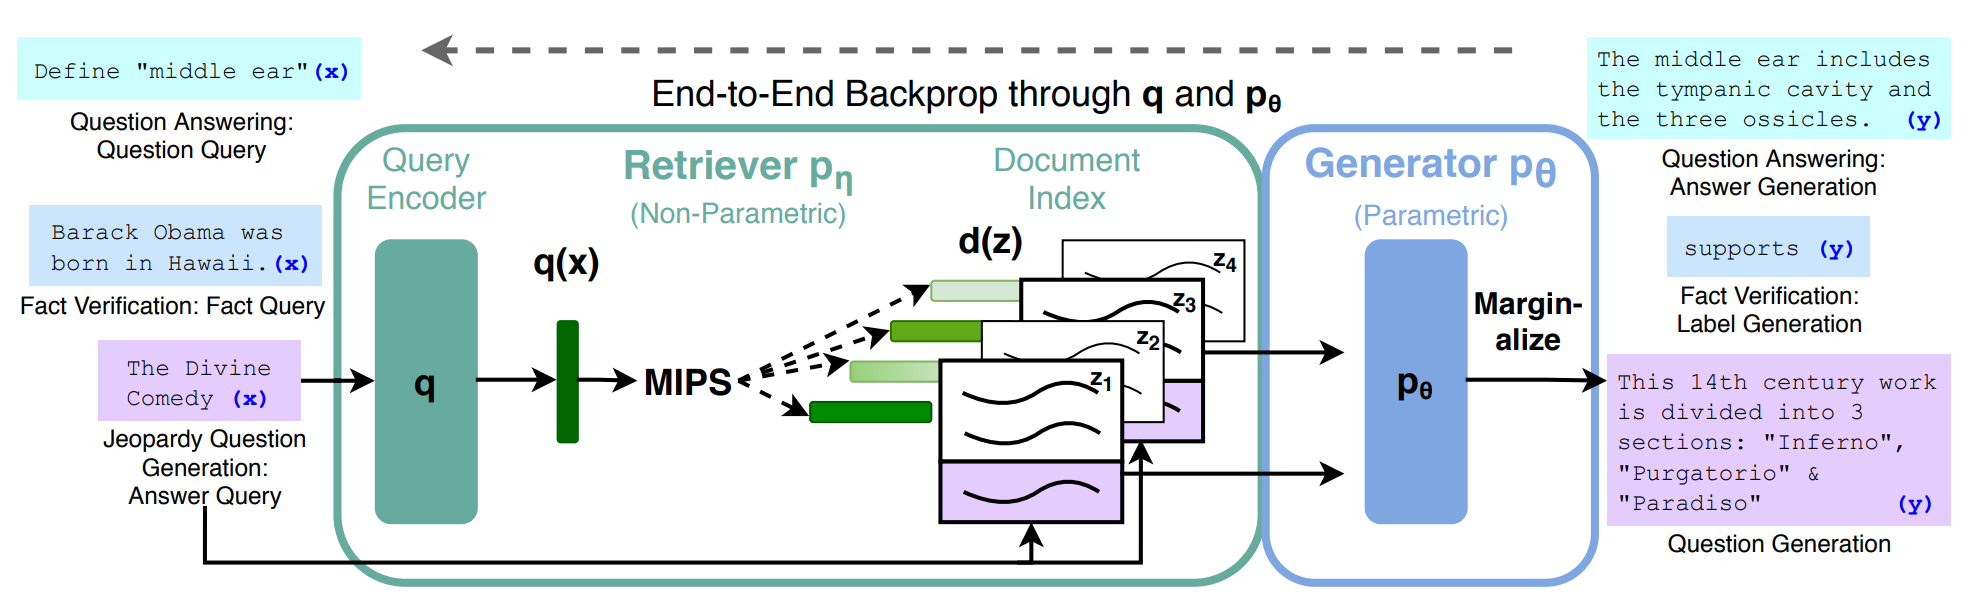
\includegraphics[width=\textwidth]{../images/image011}
				\caption{شبیه سازی \lr{RAG} پایه}
				\label{RAG_Basic}
			\end{figure}
			
			\subsection{\lr{Vector Database RAG}} \label{Vector_Rag}
				\lr{RAG}
				مبتنی بر پایگاه داده برداری یکی از روش‌های متداول در \lr{RAG} سیستم‌ها است که از بردارهای معنایی برای نمایش متن‌ها و جستجوی مفهومی بهره می‌برد. این روش با تکیه بر تبدیل اسناد و پرسش‌ها به بردارهایی در فضای برداری، امکان بازیابی سریع و مرتبط اطلاعات از پایگاه‌های داده بزرگ را فراهم می‌کند. فرایند کلی این نوع \lr{RAG} شامل سه مرحله اصلی است: ایندکس‌گذاری، بازیابی، و تولید پاسخ. 
				\cite{xiong_benchmarking_2024} \cite{gao_retrieval-augmented_2024}
				
				در مرحله ایندکس‌گذاری، داده‌های خام به بخش‌های کوچک‌تر تقسیم شده و هر بخش با استفاده از مدل‌های \lr{embedding} به بردار معنایی تبدیل می‌شود. این بردارها که معنا و زمینه متن را به صورت فشرده نمایش می‌دهند، در یک پایگاه داده برداری ذخیره می‌شوند. داده‌هایی مانند منبع متن، شماره صفحه، و تاریخ نیز برای بهبود دقت و فیلتر کردن نتایج در این پایگاه ذخیره می‌شوند.
				
				بازیابی در \lr{RAG} برداری با تطبیق پرسش کاربر با بردارهای ذخیره‌شده در پایگاه داده انجام می‌شود. ابتدا پرسش کاربر با همان مدل \lr{embedding} به بردار تبدیل می‌شود. سپس پایگاه داده برداری نزدیک‌ترین بردارهای مرتبط را بر اساس معیارهای شباهت معنایی مانند شباهت کسینوسی جستجو می‌کند. چانک‌های متنی که بالاترین امتیاز شباهت را دارند، به عنوان نتایج بازیابی‌شده انتخاب می‌شوند و آماده ارائه به مدل زبانی بزرگ می‌گردند.
				
				در مرحله نهایی، یعنی تولید پاسخ، پرسش و بخش‌های بازیابی‌شده ترکیب شده و به صورت یک پرامپت به مدل زبانی بزرگ ارسال می‌شوند. مدل با تحلیل این پرامپت، پاسخی منسجم و مبتنی بر اطلاعات بازیابی‌شده تولید می‌کند. این پاسخ می‌تواند هم دقیق باشد و هم با زمینه معنایی پرسش مطابقت داشته باشد، زیرا از داده‌های خارجی برای تولید آن استفاده شده است. در تصویر \ref{RAG_strcuture} مراحل اجرا توصیف شده است.
				
				\begin{figure}[ht]
					\centering
					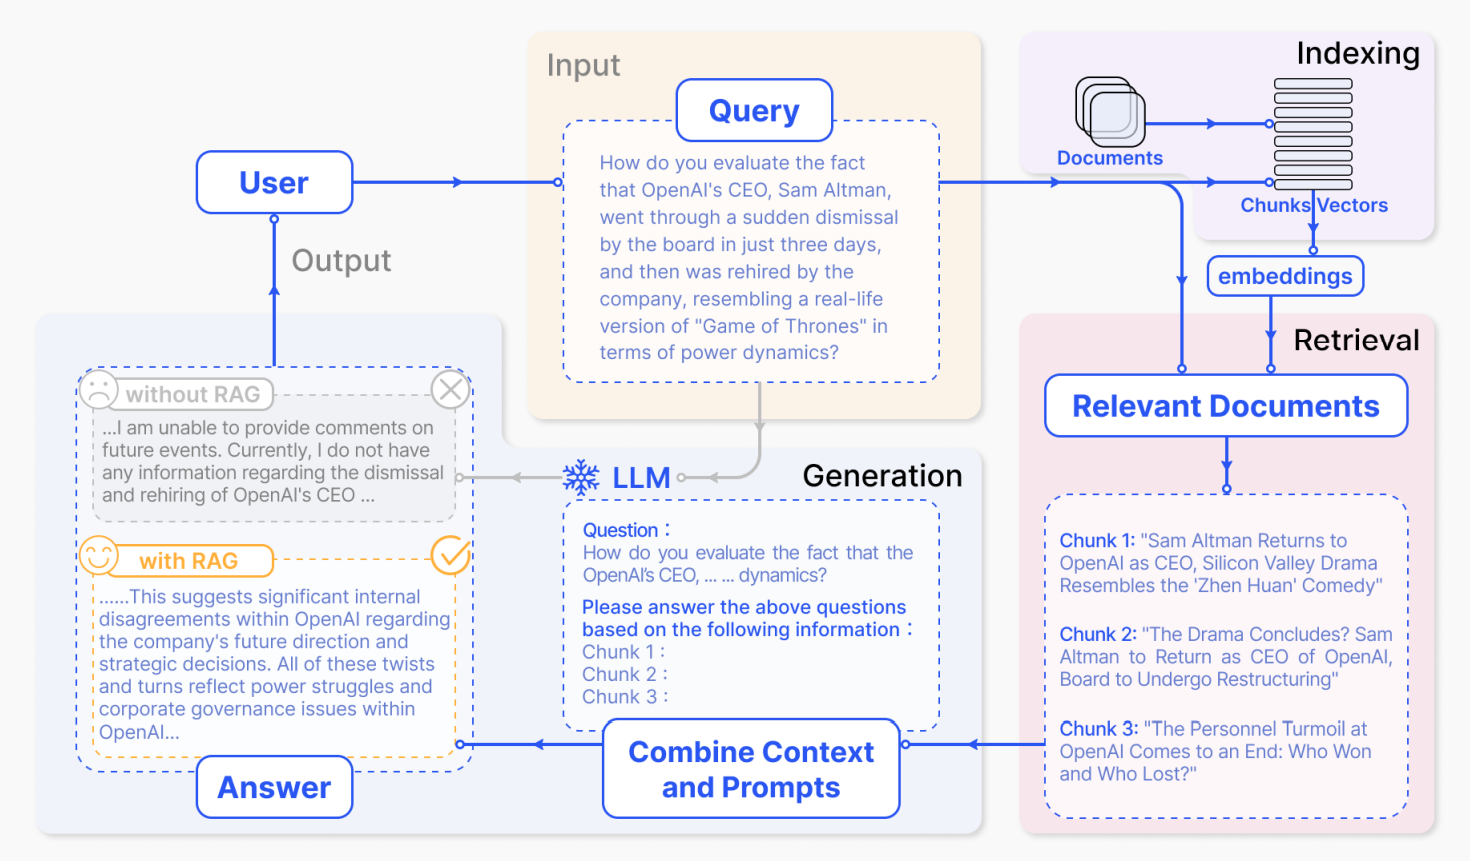
\includegraphics[width=\textwidth]{../images/image013}
					\caption{روند اجرا و استفاده از \lr{Vector Database RAG}}
					\label{RAG_strcuture}
				\end{figure}
				
				مزیت‌های \lr{RAG} برداری شامل سرعت بالا، انعطاف‌پذیری در جستجوی مفهومی، و سازگاری با انواع داده‌های متنی است. این سیستم‌ها می‌توانند حتی در صورت عدم تطابق دقیق کلمه‌به‌کلمه بین پرسش و متن‌های موجود، اطلاعات مرتبط را بازیابی کنند. همچنین، پایگاه داده برداری امکان مدیریت حجم زیادی از داده‌ها را با کارایی بالا فراهم می‌کند.  
				
				با این حال، این روش محدودیت‌هایی نیز دارد. از جمله این محدودیت‌ها می‌توان به ناتوانی در درک روابط پیچیده بین موجودیت‌ها و ضعف در پاسخ به سوالات چندمرحله‌ای اشاره کرد. همچنین، هزینه‌های ذخیره‌سازی و محاسبات مرتبط با بردارها در پایگاه‌های داده بزرگ ممکن است چالش‌برانگیز باشد. برای غلبه بر این محدودیت‌ها، بهبودهایی مانند بهینه‌سازی استراتژی‌های ایندکس‌گذاری، استفاده از فراداده‌ها، و تکنیک‌های پیش‌بازیابی و پس‌بازیابی پیشنهاد شده است.
				
				\lr{RAG}
				مبتنی بر پایگاه داده برداری در کاربردهای متنوعی مانند چت‌بات‌ها، تحلیل اسناد علمی، و مدیریت دانش در سازمان‌ها استفاده می‌شود. این روش با فراهم کردن بازیابی سریع و مرتبط اطلاعات، به کاربران کمک می‌کند تا به پاسخ‌های دقیق و معنادار دست یابند. اگر چه محدودیت‌هایی دارد، اما همچنان یکی از روش‌های محبوب و موثر در سیستم‌های بازیابی اطلاعات و تولید متن به شمار می‌آید.
				
				
			\subsection{\lr{Graph RAG}} \label{GraphRAG}
				
				\lr{Graph RAG}
				یکی از رویکردهای پیشرفته در سیستم‌ها \lr{RAG} است که از گراف‌ها به عنوان ابزار اصلی برای نمایش روابط پیچیده میان موجودیت‌ها و مفاهیم استفاده می‌کند. روند اجرای این روش در تصویر \ref{GraphRAG_strcuture} توصیف شده است. \cite{edge_local_2024}
				\begin{figure}[ht]
					\centering
					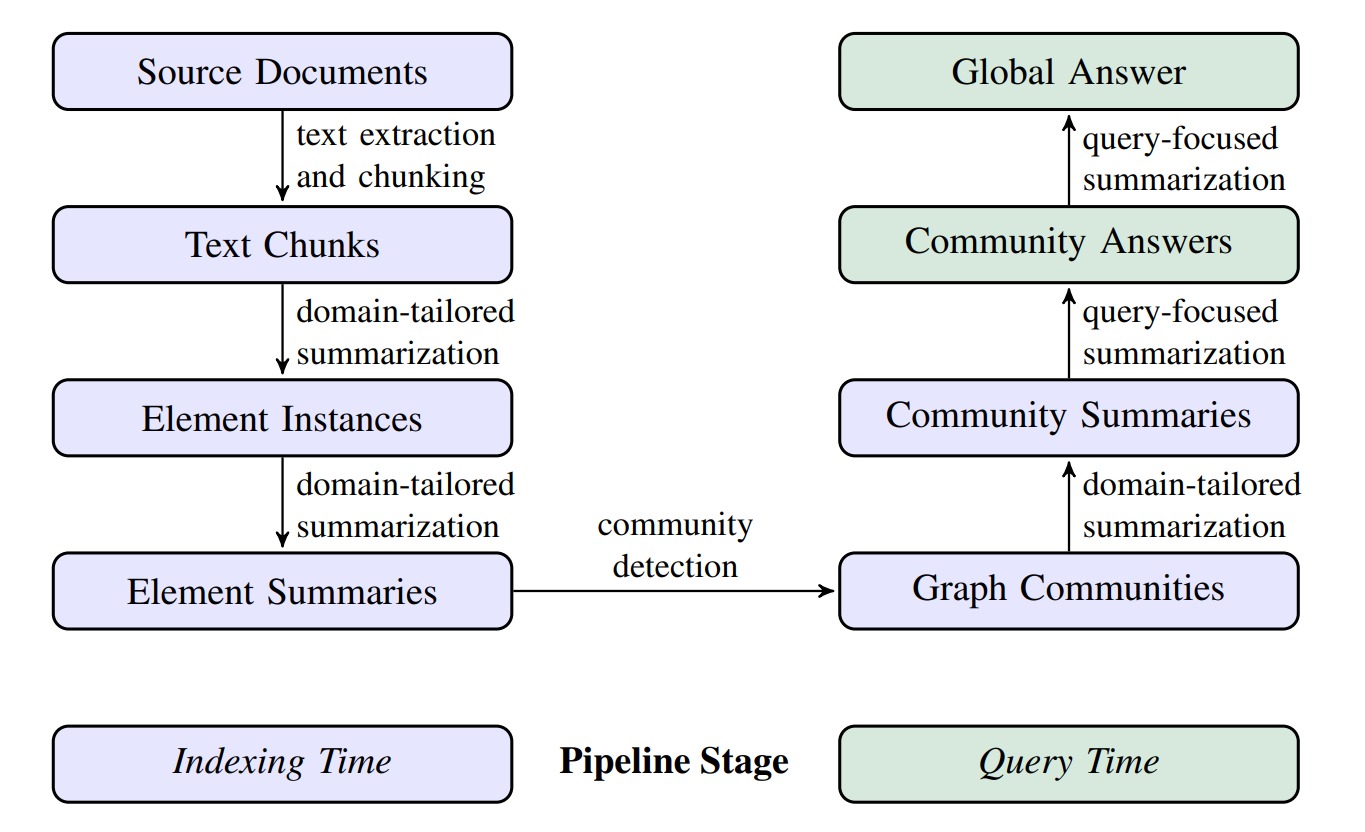
\includegraphics[width=0.8\textwidth]{../images/image017}
					\caption{روند اجرا و استفاده از \lr{Graph RAG}}
					\label{GraphRAG_strcuture}
				\end{figure}
				
				
				\lr{Graph RAG}
				بر اساس ایده استفاده از ساختارهای گرافی برای نمایش روابط میان موجودیت‌ها در مجموعه داده‌های متنی توسعه یافته است. گراف‌ها قادر به نمایش ارتباطات و وابستگی‌های پیچیده میان عناصر مختلف هستند، چیزی که در روش \ref{Vector_Rag} کمتر مورد توجه قرار می‌گیرد. با استفاده از گراف، سیستم می‌تواند نه تنها اطلاعات مرتبط را بازیابی کند، بلکه روابط میان این اطلاعات را نیز در نظر بگیرد، که این امر در پاسخ به پرسش‌های چندوجهی و پیچیده اهمیت بالایی دارد.
				
				در رویکرد \lr{Graph RAG}، ابتدا داده‌های متنی به قطعات کوچک‌تر تقسیم می‌شوند و سپس این قطعات برای استخراج موجودیت‌ها (مانند اشخاص، مکان‌ها یا مفاهیم) و روابط میان آن‌ها مورد تجزیه‌وتحلیل قرار می‌گیرند. این موجودیت‌ها و روابط در قالب گراف نمایش داده می‌شوند، که هر گره نشان‌دهنده یک موجودیت و هر یال نمایانگر رابطه میان موجودیت‌ها است. برای اطمینان از کیفیت و دقت گراف، از تکنیک‌های خلاصه‌سازی و حذف افزونگی استفاده می‌شود تا داده‌ها بهینه‌سازی شوند.
				
				یکی از ویژگی‌های کلیدی \lr{Graph RAG} استفاده از الگوریتم‌های شناسایی اجتماعات گرافی مانند الگوریتم لیدن است. این الگوریتم‌ها گراف را به بخش‌هایی تقسیم می‌کنند که هر بخش شامل موجودیت‌ها و روابط به‌هم‌پیوسته است (تصویر \ref{GraphRAG_subGraph}). سپس برای هر بخش خلاصه‌ای تولید می‌شود که دیدگاهی جامع از اطلاعات موجود در آن بخش ارائه می‌دهد. این خلاصه‌ها به سیستم اجازه می‌دهد تا در زمان پاسخگویی به پرسش‌های کاربر، به سرعت بخش‌های مرتبط را پیدا کند.
				
				\begin{figure}[ht]
					\centering
					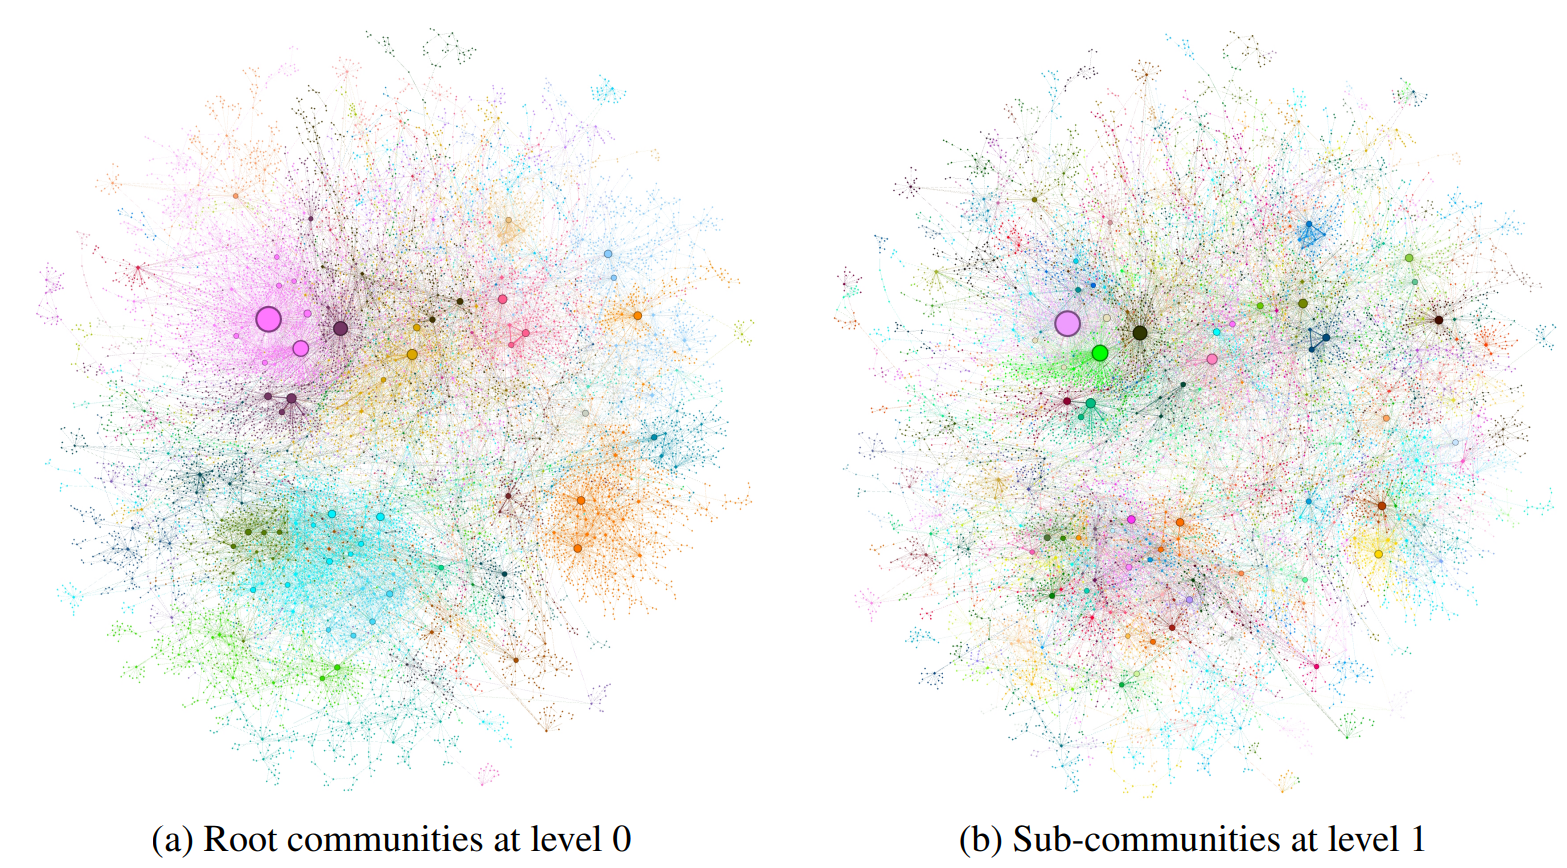
\includegraphics[width=\textwidth]{../images/image018}
					\caption{تقسیم گراف به یخش‌هایی مختلف}
					\label{GraphRAG_subGraph}
				\end{figure}
							
				\lr{Graph RAG}
				از خلاصه‌های گرافی برای تولید پاسخ‌های جامع و متناسب با پرسش‌های کاربران استفاده می‌کند. این سیستم ابتدا هر اجتماع گرافی را به صورت مستقل تحلیل می‌کند و پاسخ‌هایی جزئی تولید می‌کند. سپس این پاسخ‌های جزئی به یک پاسخ کلی ترکیب می‌شوند که نمایانگر دیدگاهی جامع و مرتبط با پرسش اصلی است. این فرآیند به ویژه در پاسخ‌گویی به پرسش‌هایی که نیازمند جمع‌آوری و تلفیق اطلاعات از منابع مختلف هستند، کاربرد دارد.
				
				
				\lr{Graph RAG}
				در مقایسه با روش \ref{Vector_Rag}، دقت و جامعیت بالاتری در پاسخ‌گویی به پرسش‌های پیچیده ارائه می‌دهد. همچنین، استفاده از ساختار گرافی امکان تحلیل بهتر روابط میان داده‌ها را فراهم می‌کند. با این حال، ایجاد و مدیریت گراف‌های بزرگ ممکن است هزینه‌های محاسباتی بیشتری به همراه داشته باشد، و همچنین نیازمند طراحی دقیق برای به‌روزرسانی و مدیریت اطلاعات جدید است.
				
					
			\subsection{\lr{Light RAG}}
			
				\lr{LightRAG}
					یک چارچوب پیشرفته در حوزه تولید تقویت‌شده با بازیابی \lr{RAG} است که با استفاده از ساختارهای گرافی و روش‌های بازیابی دو سطحی، محدودیت‌های موجود در سیستم‌های قبلی را برطرف می‌کند. این رویکرد بهینه‌سازی شده، بازیابی اطلاعات را کارآمدتر، دقیق‌تر و انعطاف‌پذیرتر می‌سازد و نیازهای متنوع کاربران را پاسخ می‌دهد. روند کار \lr{LightRAG} در تصویر \ref{LightRAG_subGraph} تصویر سازی شده است. 
					
					\begin{figure}[ht]
						\centering
						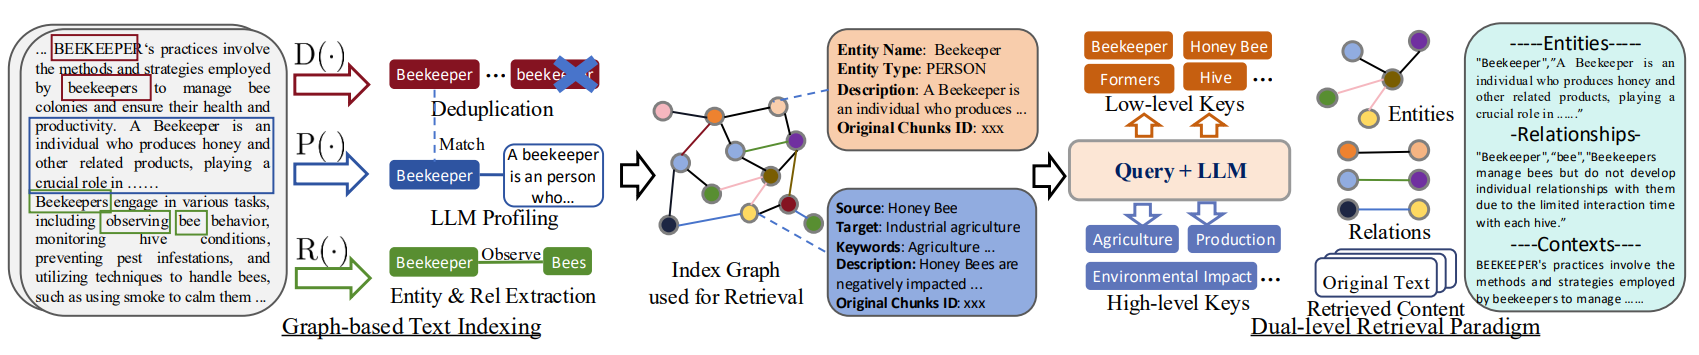
\includegraphics[width=\textwidth]{../images/image019}
						\caption{تقسیم گراف به یخش‌هایی مختلف}
						\label{LightRAG_subGraph}
					\end{figure}
				

				یکی ویژگی‌های \lr{LightRAG}، استفاده از گراف‌های دانش مانند روش \ref{GraphRAG} برای سازماندهی و مدیریت اطلاعات است. در این روش، اسناد به بخش‌های کوچک‌تری تقسیم می‌شوند و با استفاده از مدل‌های زبانی بزرگ، موجودیت‌ها، روابط و اطلاعات مرتبط استخراج می‌شوند. این عناصر در قالب یک گراف ساختاریافته ذخیره می‌شوند، به‌طوری که گره‌ها نمایانگر موجودیت‌ها و یال‌ها نشان‌دهنده روابط بین آن‌ها هستند. فرایند حذف داده‌های تکراری نیز برای بهینه‌سازی اندازه و عملکرد گراف اجرا می‌شود. این روش امکان تحلیل روابط پیچیده و بازیابی اطلاعات چندمنبعی را فراهم می‌کند.
				
				\lr{LightRAG}
				از یک روش بازیابی دو سطحی استفاده می‌کند که هم به سوالات جزئی و هم به سوالات کلی پاسخ می‌دهد. 
				
				\begin{itemize}
					
					\item {\large بازیابی سطح پایین}: 
					این سطح به بازیابی دقیق اطلاعات درباره موجودیت‌ها و روابط خاص می‌پردازد. برای مثال، سوالاتی مانند «چه کسی نویسنده کتاب غرور و تعصب است؟» در این سطح پاسخ داده می‌شود.
					بازیابی سطح بالا: این سطح بر استخراج اطلاعات کلی‌تر و موضوعات گسترده‌تر تمرکز دارد و برای پاسخ‌گویی به سوالاتی مانند «هوش مصنوعی چگونه بر آموزش مدرن تأثیر می‌گذارد؟» مناسب است.
					
					\item {\large بازیابی سطح بالا}: 
					این سطح بر استخراج اطلاعات کلی‌تر و موضوعات گسترده‌تر تمرکز دارد و برای پاسخ‌گویی به سوالاتی مانند «هوش مصنوعی چگونه بر آموزش مدرن تأثیر می‌گذارد؟» مناسب است.
					این دو سطح با هم کار می‌کنند تا پاسخ‌های دقیق و جامع ارائه دهند.
					
				\end{itemize}


				\lr{LightRAG}
				با ادغام ساختارهای گرافی و \lr{vector embeddings}، یعنی ادغام روش‌های \ref{Vector_Rag} و \ref{GraphRAG} بازیابی اطلاعات را بهینه می‌کند. کلیدواژه‌های محلی و کلی از پرسش استخراج می‌شوند و برای شناسایی موجودیت‌ها و روابط مرتبط به کار می‌روند. این روش نه تنها ارتباطات مستقیم، بلکه روابط چندلایه را نیز بازیابی می‌کند و کیفیت پاسخ‌ها را بهبود می‌بخشد.
				

				یکی از ویژگی‌های برجسته \lr{LightRAG}، قابلیت به‌روزرسانی سریع و تدریجی گراف دانش است. به جای بازسازی کامل گراف (ایراد اصلی روش \ref{GraphRAG})، داده‌های جدید به ساختار موجود اضافه می‌شوند. این ویژگی باعث کاهش هزینه‌های پردازشی و حفظ یکپارچگی داده‌های قدیمی می‌شود. این رویکرد تضمین می‌کند که سیستم همیشه به‌روز و دقیق باقی بماند، حتی در محیط‌هایی که داده‌ها به‌طور مداوم تغییر می‌کنند. 
				
				مزایای کلیدی \lr{LightRAG} عبارت است از:
				
				\begin{itemize}
					
					\item {\large جامعیت بیشتر}:
					ساختار گرافی به \lr{LightRAG} امکان می‌دهد تا اطلاعات جامع و روابط میان‌متنی را استخراج کرده و پاسخ‌های عمیق‌تری ارائه دهد.
					
					\item {\large کارایی بالا}:
					با ترکیب گراف و بردارها، این سیستم سرعت پردازش را افزایش داده و هزینه‌ها را کاهش می‌دهد.
					
					\item {\large انعطاف‌پذیری}:
					قابلیت به‌روزرسانی تدریجی سیستم را به ابزاری مناسب برای محیط‌های پویا تبدیل کرده است.
					
					\item {\large مقیاس‌پذیری}:
					این سیستم برای کاربردهایی با حجم بالای داده‌ها مناسب است و در حوزه‌های مختلف مانند پزشکی، آموزش و مدیریت دانش قابل استفاده است.
					
				\end{itemize}


				\lr{LightRAG}
				یک نوآوری مهم در حوزه \lr{RAG} است که با ترکیب ساختارهای گرافی، بازیابی دو سطحی، و الگوریتم‌های به‌روزرسانی تدریجی، مشکلات سیستم‌های قبلی را حل کرده و کارایی و دقت را بهبود داده است. این سیستم برای کاربردهایی مانند تحلیل داده‌های پویا، پاسخ‌گویی به سوالات چندمنبعی، و مدیریت دانش در سازمان‌ها، راه‌حلی ایده‌آل ارائه می‌دهد. \cite{guo_lightrag_2024}
				
			\subsection{اعمال \lr{RAG} روی مدل}
			
				در این پروژه از \lr{LightRAG} استفاده می‌شود زیرا شامل هردو روش قبلی می‌شود و مشکلات روش‌های دیگر را بطور کامل حل کرده است. مقایسه این سه روش در جدول \ref{RAG_comparison} قرار دارد.
				
				\begin{table}[h!]
					\centering
					\begin{adjustbox}{max width=\textwidth}
						\begin{tabular}{|p{3cm}|p{4cm}|p{4cm}|p{4cm}|}
							\hline
							\textbf{ویژگی‌ها} & \textbf{\lr{Vector Database RAG}} & \textbf{\lr{Graph RAG}} & \textbf{\lr{text}} \\ \hline
							\textbf{ساختار داده} & 
							نمایش برداری از متن و ذخیره‌سازی در پایگاه داده برداری & 
							گراف‌های دانش شامل گره‌ها (موجودیت‌ها) و یال‌ها (روابط) & 
							گراف دانش سبک با روش‌های شاخص‌گذاری و بازیابی دو سطحی \\ \hline
							
							\textbf{روش بازیابی} & 
							جستجو بر اساس نزدیکی برداری (\lr{similarity search}) & 
							شناسایی موجودیت‌ها و روابط از طریق اجتماع‌های گرافی & 
							بازیابی دو سطحی: بازیابی دقیق (سطح پایین) و موضوعی (سطح بالا) \\ \hline
							
							\textbf{مزایا} & 
							سرعت بالا در جستجو و قابلیت کار با داده‌های بزرگ & 
							توانایی نمایش روابط پیچیده میان داده‌ها و ارائه خلاصه‌های چندسطحی & 
							انعطاف‌پذیری بالا، به‌روزرسانی تدریجی، و هزینه محاسباتی پایین \\ \hline
							
							\textbf{محدودیت‌ها} & 
							مشکل در مدیریت روابط پیچیده و نیاز به به‌روزرسانی‌های مداوم & 
							هزینه محاسباتی بالا و پیچیدگی در مدیریت گراف‌های بزرگ & 
							وابستگی به گراف‌های کوچک‌تر و نیاز به طراحی دقیق شاخص‌گذاری \\ \hline
							
							\textbf{کاربردها} & 
							جستجوی دانش عمومی و بازیابی متون & 
							تحلیل داده‌های پیچیده، چندمنبعی و چندموضوعی & 
							کاربردهای سریع در محیط‌های پویا و داده‌های متغیر \\ \hline
						\end{tabular}
					\end{adjustbox}
					\caption{تفاوت‌های \lr{Vector Database RAG}، \lr{Graph RAG} و \lr{Light RAG}}
					\label{RAG_comparison}
				\end{table}
				
				(ارزیابی مدل و توضیحات تکمیلی)
			
		\section{رویکردهای \lr{Prompt engineering}}
		
			در این بخش بررسی می‌کنیم که ورودی مدل چه تاثیری در پاسخ مدل دارد و چه روش‌های در این مورد استفاده می‌شود و کدام روش‌های در این پروژه مورد استفاده قرار می‌گیرد به همراه دلایل استفاده از آن.
		
			تأثیر ورودی مدل بر دقت آن عمدتاً به نحوه ارائه اطلاعات و میزان تطابق ورودی‌ها با وظایف موردنظر بستگی دارد. در مدل‌ها ورودی‌ها می‌توانند شامل مثال‌های مرتبط با وظیفه باشند که به مدل کمک می‌کنند وظیفه را بهتر درک کرده و پیش‌بینی کند. در یادگیری \lr{Zero-Shot}، مدل تنها با یک توضیح متنی وظیفه را انجام می‌دهد که چالش‌برانگیز است اما انعطاف بالایی دارد. با اضافه کردن یک یا چند مثال (یادگیری \lr{One-Shot} و \lr{Few-Shot})، مدل عملکرد بهتری از خود نشان می‌دهد، زیرا مثال‌ها به عنوان راهنمایی برای درک وظیفه عمل می‌کنند. این رویکردها نشان می‌دهند که دقت مدل به تعداد و کیفیت ورودی‌های ارائه‌شده وابسته است.  \cite{brown_language_2020} \cite{wang_prompt_2024} اما در این پروژه به این دلیل که سوالات فرم و قالب مشخصی ندارند این روش قابل استفاده نیست.
			
			علاوه بر این، اندازه مدل و مجموعه داده‌های آموزشی نیز بر عملکرد آن تأثیر زیادی دارد. افزایش تعداد پارامترهای مدل و ارائه داده‌های متنوع و با کیفیت، توانایی مدل را در شناسایی الگوهای پیچیده و انجام وظایف متنوع افزایش می‌دهد. با این حال، کیفیت ورودی‌ها و ارتباط آن‌ها با وظیفه همچنان اهمیت دارد؛ داده‌های ناهماهنگ می‌توانند دقت مدل را کاهش دهند. بنابراین، ورودی‌های مناسب و طراحی‌شده با دقت، نقش کلیدی در بهبود عملکرد مدل‌های زبانی ایفا می‌کنند.
			
			در ادامه روش‌های استدلالی را بررسی می‌کنیم که در مقالات بخش \ref{related_works} هم از این روش‌ها استفاده کرده اند.
			
			\subsection{\lr{CoT}} \label{CoT}
			
				روش \lr{Chain-of-Thought Prompting} یک تکنیک ساده اما قدرتمند برای بهبود توانایی استدلال مدل‌های زبانی بزرگ است. در این روش، به جای ارائه مستقیم سؤال و پاسخ، زنجیره‌ای از استدلال‌های میانی که منجر به پاسخ نهایی می‌شوند، به مدل ارائه می‌شود. این زنجیره‌ها به مدل کمک می‌کنند مسائل پیچیده را به مراحل ساده‌تر تقسیم کند و به طور گام‌به‌گام به پاسخ برسد. از مزایای این روش می‌توان به امکان تجزیه مسائل چندمرحله‌ای، ایجاد شفافیت در فرآیند استدلال و کاربرد آن در مسائل متنوعی مانند ریاضی، استدلال عقلانی و مسائل نمادین اشاره کرد. این روش به راحتی با چند نمونه‌ی آماده در مدل‌های بزرگ قابل پیاده‌سازی است و نیازی به آموزش‌های پیچیده ندارد. مثال استفاده از این روش در شکل \ref{CoT_vs_normal}.
				
				\begin{figure}[ht]
					\centering
					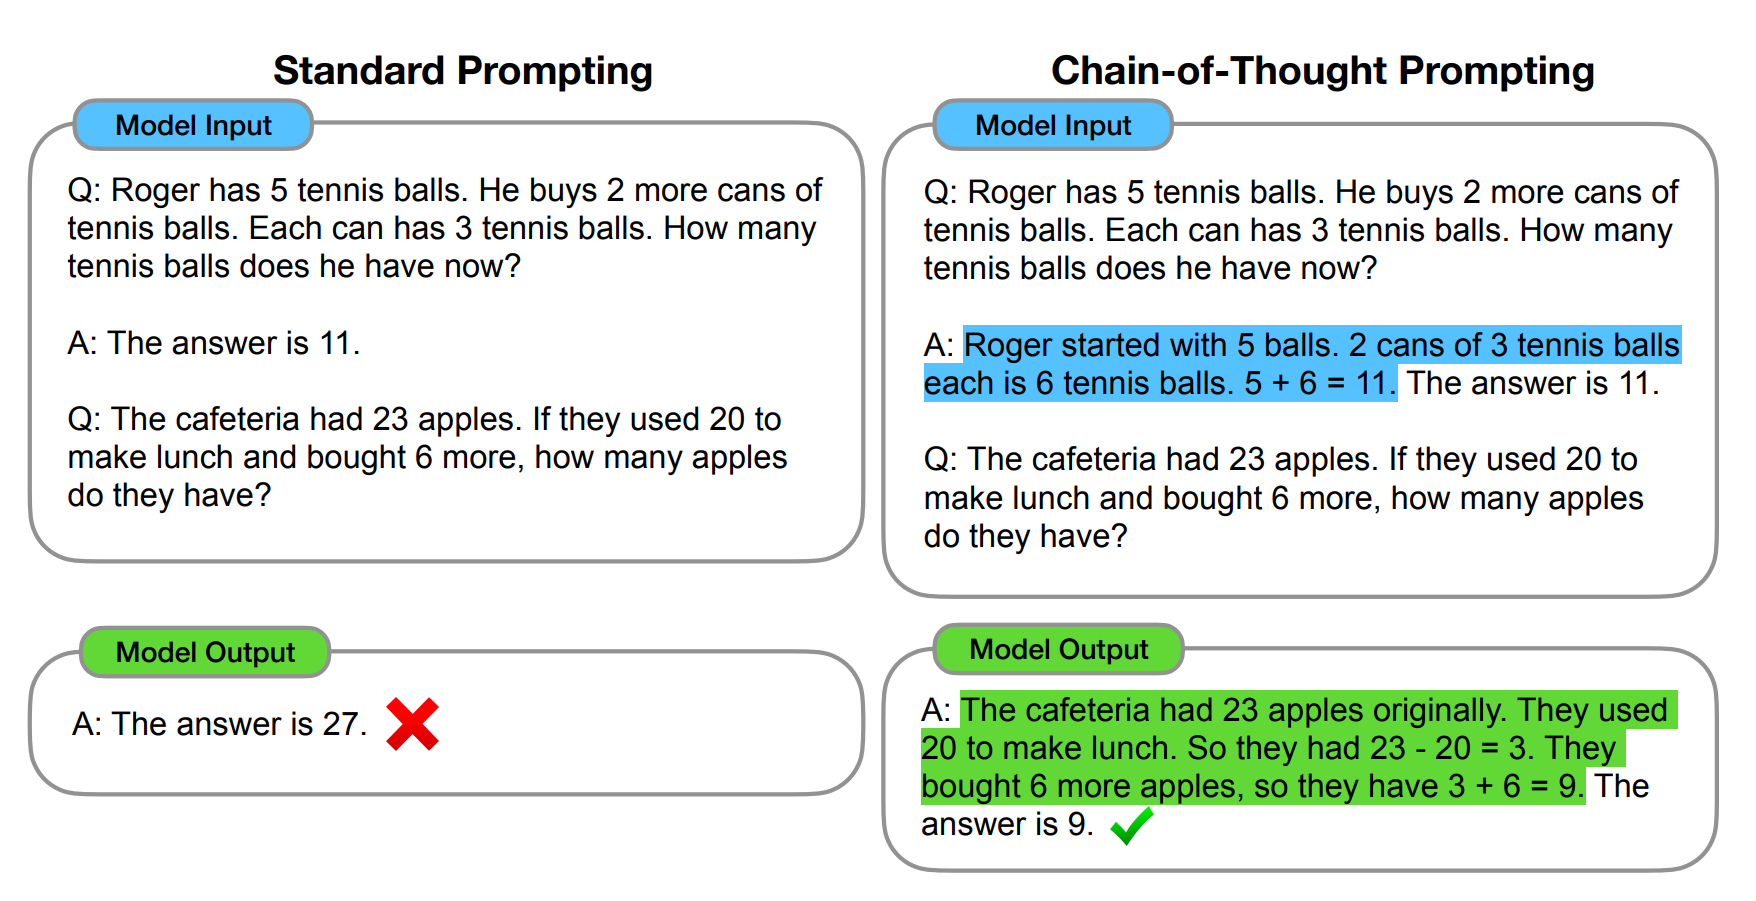
\includegraphics[width=\textwidth]{../images/image020}
					\caption{مقایسه ورودی \lr{CoT} با ورودی عادی}
					\label{CoT_vs_normal}
				\end{figure}
				
				آزمایش‌ها نشان داده‌اند که \lr{Chain-of-Thought Prompting} در مدل‌های با ابعاد بسیار بزرگ (حدود 100 میلیارد پارامتر یا بیشتر) عملکرد چشمگیری در حل مسائل پیچیده دارد. به عنوان مثال، این روش در مجموعه داده‌های ریاضی مانند \lr{GSM8K} و مسائل استدلالی دیگر، باعث افزایش قابل‌توجه دقت مدل شده است. برخلاف روش‌های استاندارد که مدل‌ها را مستقیم به سمت پاسخ هدایت می‌کنند، این تکنیک از ارائه مراحل میانی استدلال بهره می‌برد که نه تنها عملکرد را بهبود می‌بخشد، بلکه فرآیند تصمیم‌گیری مدل را شفاف‌تر و قابل بررسی می‌کند. \cite{wei_chain--thought_2023}
				
			\subsection{\lr{sc-CoT}}
			
				روش \lr{Self-Consistency}، یک استراتژی جدید برای بهبود عملکرد روش زنجیره‌ای استدلال\LTRfootnote{Chain-of-Thought Prompting} در مدل‌های زبانی است که هدف آن استفاده از تنوع مسیرهای استدلالی برای افزایش دقت در وظایف پیچیده است. به جای استفاده از استنتاج حریصانه\LTRfootnote{greedy decoding} برای انتخاب یک مسیر واحد، این روش مجموعه‌ای از مسیرهای استدلال متنوع را تولید کرده و پاسخ نهایی را با محاسبه میانگین این مسیرها مشخص می‌کند. فرضیه اصلی این است که پاسخ درست معمولاً از چند مسیر مختلف به دست می‌آید و اجماع بین مسیرها می‌تواند نشان‌دهنده درستی پاسخ باشد. مشایسه این روش با روش بخش \ref{CoT} در تصویر \ref{CoT_vs_sc-CoT}.
				
				\begin{figure}[ht]
					\centering
					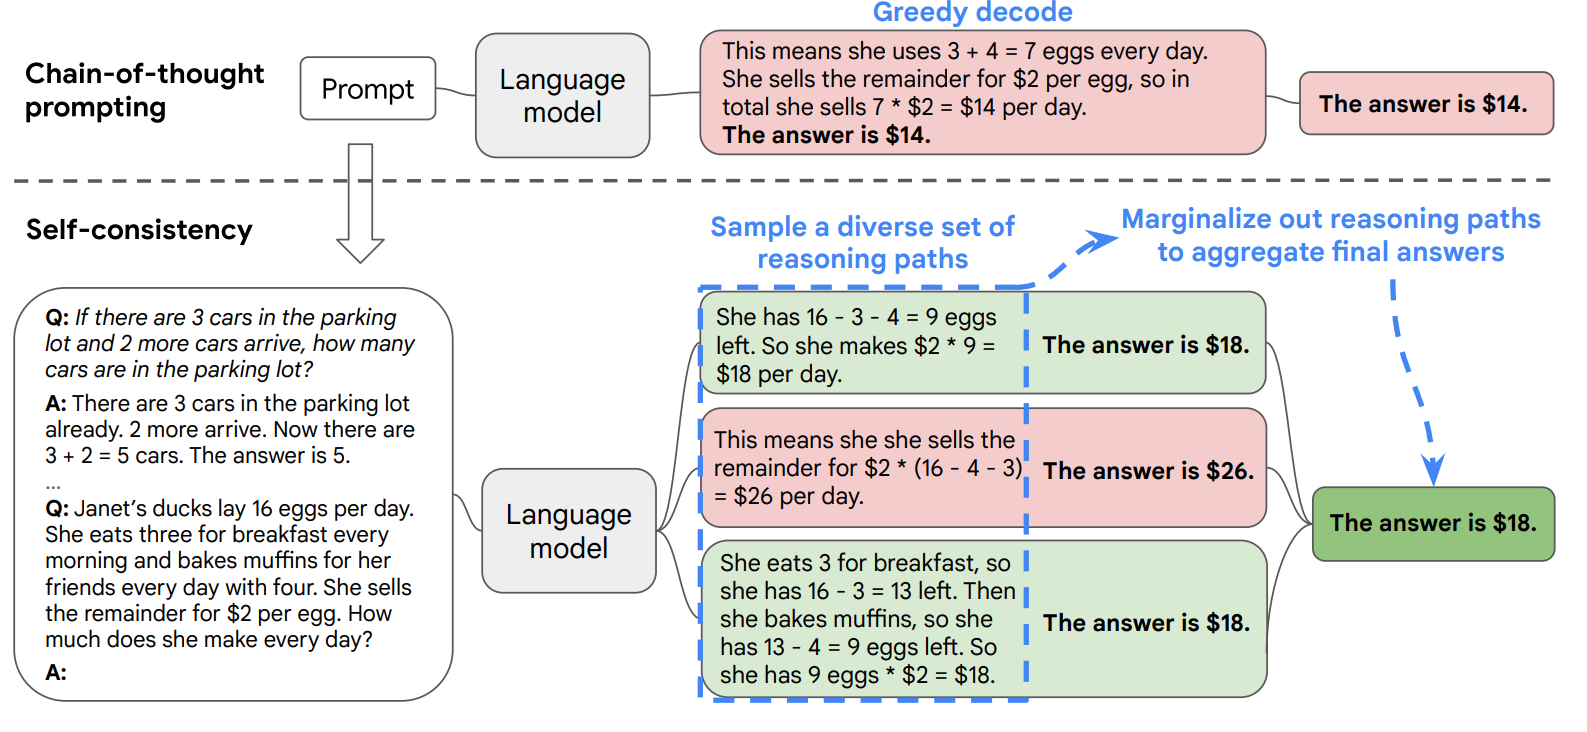
\includegraphics[width=\textwidth]{../images/image021}
					\caption{مقایسه روش \lr{CoT} با روش \lr{sc-CoT}}
					\label{CoT_vs_sc-CoT}
				\end{figure}
				
				تفاوت اصلی بین \lr{Self-Consistency} و \lr{Chain-of-Thought} در نحوه پردازش پاسخ‌ها است. در حالی که روش زنجیره‌ای استدلال به یک مسیر مشخص متکی است، \lr{Self-Consistency} مسیرهای مختلف را نمونه‌برداری کرده و پاسخ نهایی را بر اساس بیشترین توافق میان مسیرها تعیین می‌کند. این روش نیازی به آموزش اضافی یا داده‌های برچسب‌دار ندارد و می‌تواند بهبود چشمگیری در وظایف منطقی و ریاضی ایجاد کند. آزمایش‌ها نشان داده‌اند که \lr{Self-Consistency} در مدل‌های زبانی بزرگ باعث بهبود دقت قابل توجهی می‌شود و در برخی موارد عملکرد بهتری نسبت به روش‌های مرسوم مثل \lr{beam search} یا \lr{ensemble} دارد. \cite{wang_self-consistency_2023}
					
			\subsection{\lr{CoK}}
			
				روش \lr{CoK}\LTRfootnote{Chain-of-Knowledge} یک چارچوب نوآورانه است که با استفاده از منابع مختلف دانش، عملکرد مدل‌های زبانی بزرگ را در وظایف دانش‌محور بهبود می‌دهد. این روش شامل سه مرحله اصلی است: آماده‌سازی استدلال برای شناسایی دامنه‌های دانش مرتبط، انطباق پویا با دانش که اطلاعات از منابع مختلف (ساختاریافته و غیرساختاریافته) بازیابی و استدلال‌ها اصلاح می‌شوند، و تجمیع پاسخ که پاسخ نهایی بر اساس استدلال‌های اصلاح‌شده تولید می‌شود. \lr{CoK} به دلیل استفاده از اطلاعات خارجی و اصلاح تدریجی استدلال‌ها، میزان انتشار خطا را کاهش داده و دقت بیشتری در تولید پاسخ فراهم می‌کند. این روش در وظایف پیچیده مانند مسائل پزشکی و علمی، که نیاز به استفاده از دانش دقیق و به‌روز دارند، عملکرد برجسته‌ای داشته است. چارچوب این روش  در تصویر \ref{CoK_structure}. \cite{li_chain--knowledge_2024}
				
				\begin{figure}[ht]
					\centering
					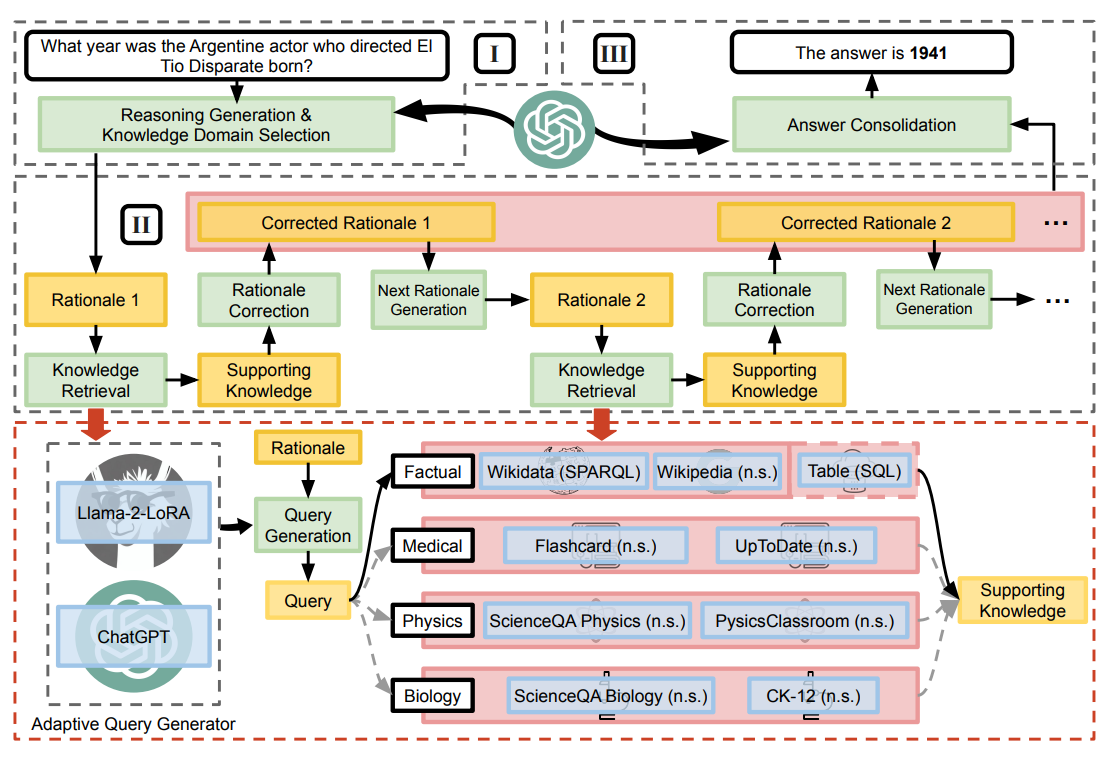
\includegraphics[width=\textwidth]{../images/image023}
					\caption{چارچوب زنجیره‌ای از دانش (\lr{CoK})، شامل (\lr{I}) آماده‌سازی استدلال، (\lr{II}) تطبیق دانش پویا، و (\lr{III}) یکپارچه‌سازی پاسخ است.}
					\label{CoK_structure}
				\end{figure}
				
				در مقایسه، روش‌های  \lr{CoT} و \lr{sc-CoT} بر تولید زنجیره‌های استدلال مبتنی بر دانش داخلی مدل تمرکز دارند. \lr{CoT} استدلال‌ها را گام‌به‌گام ارائه می‌کند، اما بدون دسترسی به منابع خارجی، ممکن است اطلاعات نادرست تولید کند. \lr{Self-Consistency} با تولید مسیرهای مختلف استدلال و انتخاب پاسخ با بیشترین اجماع، دقت بیشتری دارد، اما همچنان به دانش خارجی وابسته نیست. در مقابل، \lr{CoK} با انطباق پویا و بازیابی اطلاعات از منابع خارجی، دقت و صحت بیشتری به‌ویژه در وظایف دانش‌محور ارائه می‌دهد و بر مشکلاتی مانند توهم مدل‌ها غلبه می‌کند. مقایسه این چند روش در تصویر \ref{CoT_vs_sc-CoT_vs_CoK}.
				
				\begin{figure}[ht]
					\centering
					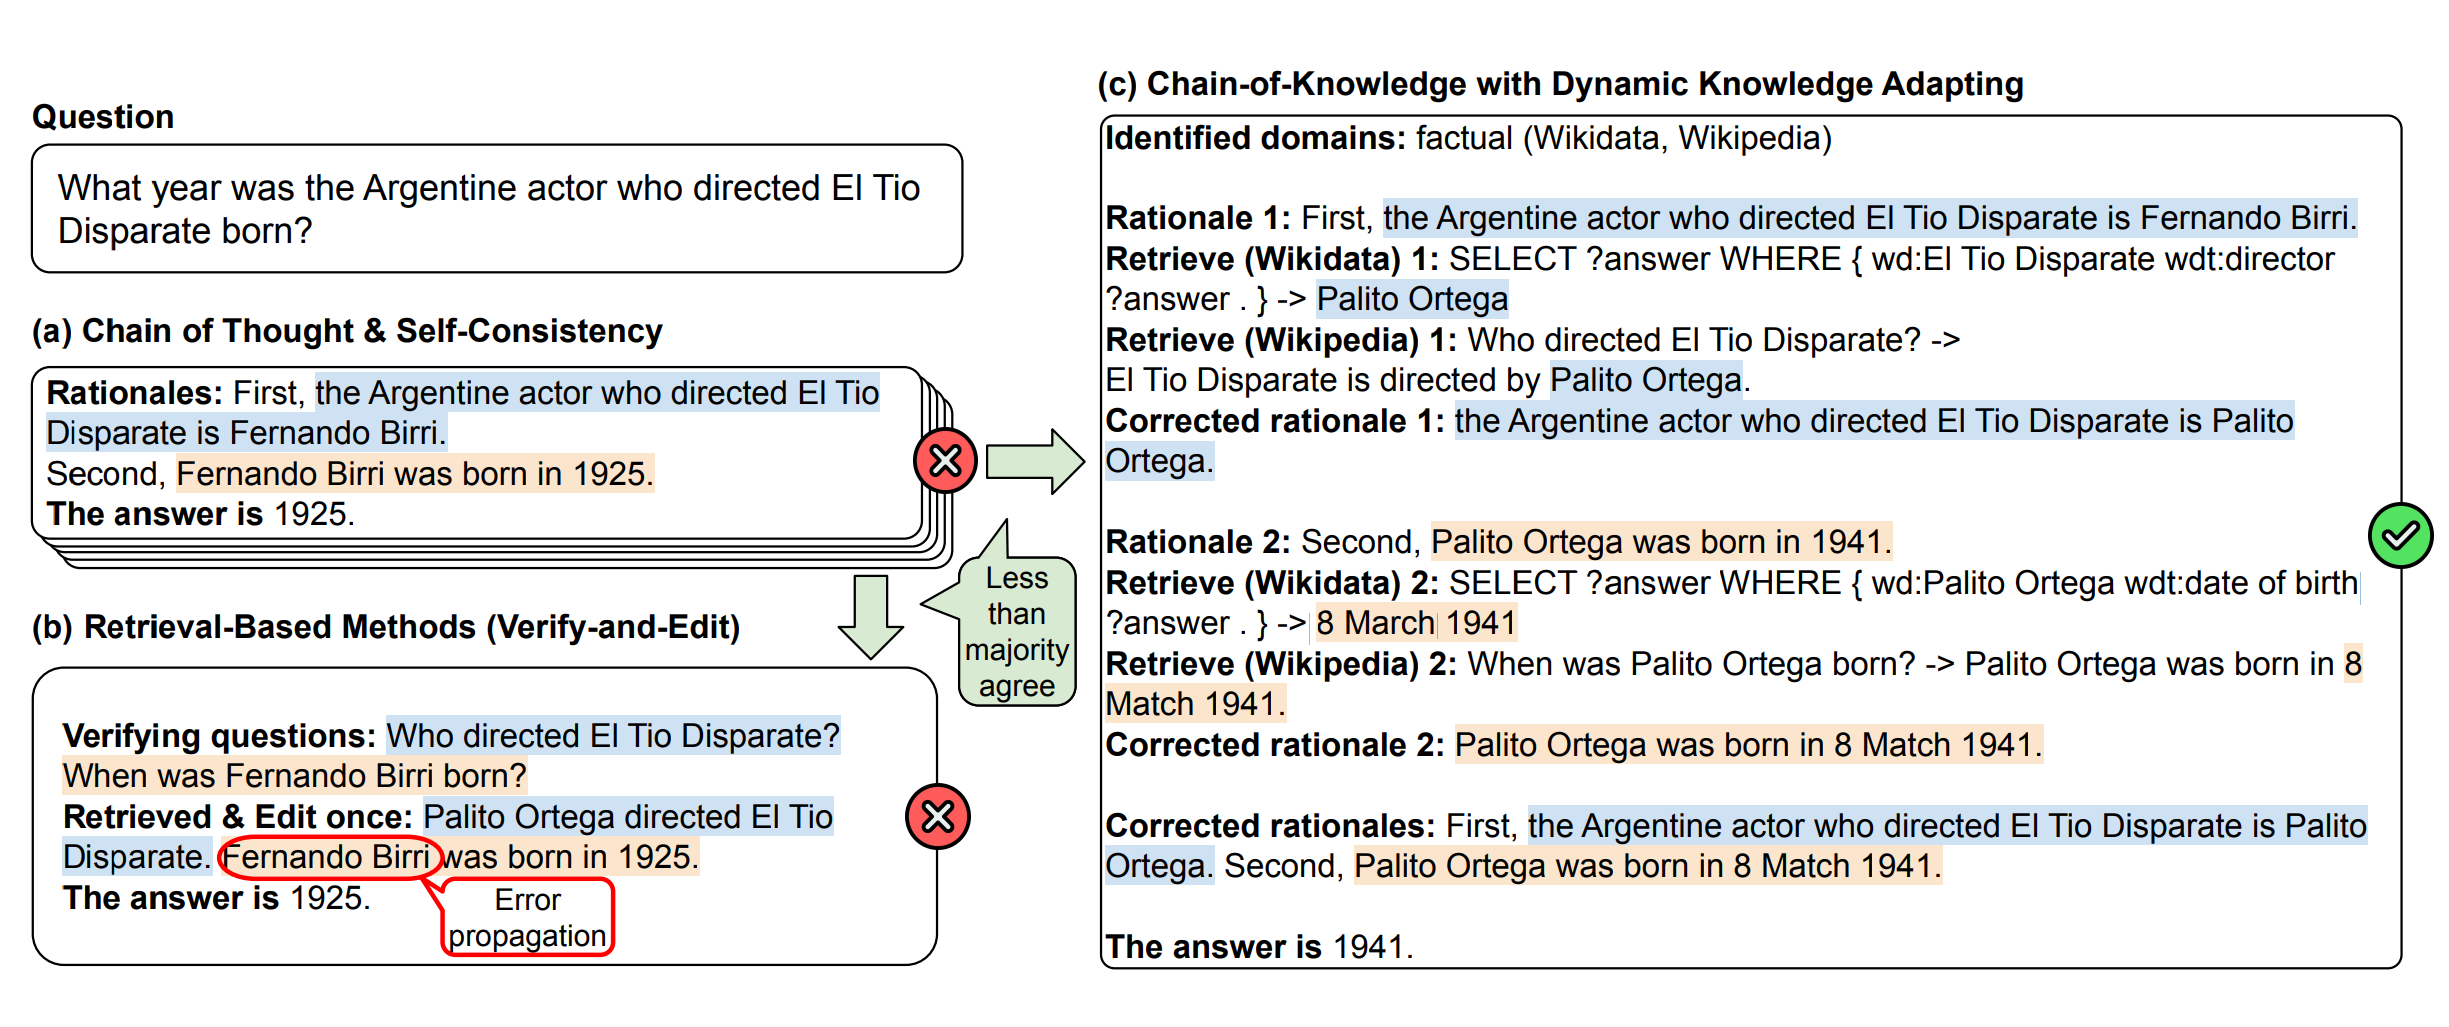
\includegraphics[width=\textwidth]{../images/image022}
					\caption{مقایسه روش \lr{CoT} روش، \lr{sc-CoT} و روش \lr{CoK}}
					\label{CoT_vs_sc-CoT_vs_CoK}
				\end{figure}
				
				این روش در صورت عدم استفاده از بخش \ref{label} روش مفیدی بود ولی در اینجا به دلیل استفاده از روش‌های پیشرفته \lr{RAG} از این روش استفاده نمی‌کنیم.
				
			\subsection{\lr{ToT}}
				
				روش \lr{ToT}\LTRfootnote{Tree of Thoughts} چارچوبی است که فرآیند استدلال مدل‌های زبانی را از یک زنجیره خطی (مانند \ref{CoT}) به یک ساختار درختی گسترش می‌دهد. در این روش، مسئله به‌صورت یک درخت استدلال مدل‌سازی می‌شود که هر گره نمایانگر یک وضعیت جزئی و هر شاخه نشان‌دهنده یک گام استدلال است. مدل به جای انتخاب یک مسیر ثابت، می‌تواند چندین مسیر را به‌طور موازی کاوش کند، با استفاده از الگوریتم‌های جستجو مانند \lr{BFS}\LTRfootnote{Breadth-First Search} یا \lr{DFS}\LTRfootnote{Depth-First Search}. این ساختار اجازه می‌دهد مدل به مسیرهای مختلف نگاه کرده، بازگشت کند و با ارزیابی گره‌ها، تصمیمات دقیق‌تری بگیرد. \lr{ToT} برای وظایفی که نیاز به برنامه‌ریزی، خلاقیت یا استدلال‌های غیر بدیهی دارند، مانند حل معماهای ریاضی یا نوشتار خلاقانه، بسیار مؤثر بوده است. \cite{yao_tree_2023}
				
				در مقایسه با \lr{CoT}، که فقط یک زنجیره از استدلال‌ها را ارائه می‌دهد، \lr{ToT} انعطاف‌پذیری بیشتری در کاوش مسیرهای جایگزین دارد و به دلیل ساختار درختی خود از جستجوی سیستمی بهره می‌برد. همچنین، در مقابل \lr{sc-CoT} که از چندین زنجیره استدلال مستقل استفاده می‌کند و با اجماع پاسخ می‌دهد، \lr{ToT} از جستجوهای هدایت‌شده با ارزیابی‌های لحظه‌ای برای انتخاب بهترین مسیر استفاده می‌کند. این باعث می‌شود \lr{ToT} در وظایفی که نیاز به بررسی دقیق و کاوش مسیرهای مختلف دارند، عملکرد بسیار بهتری داشته باشد. مقایسه این روش‌ها در تصویر \ref{CoT_vs_sc-CoT_vs_ToT}.
				
				\begin{figure}[ht]
					\centering
					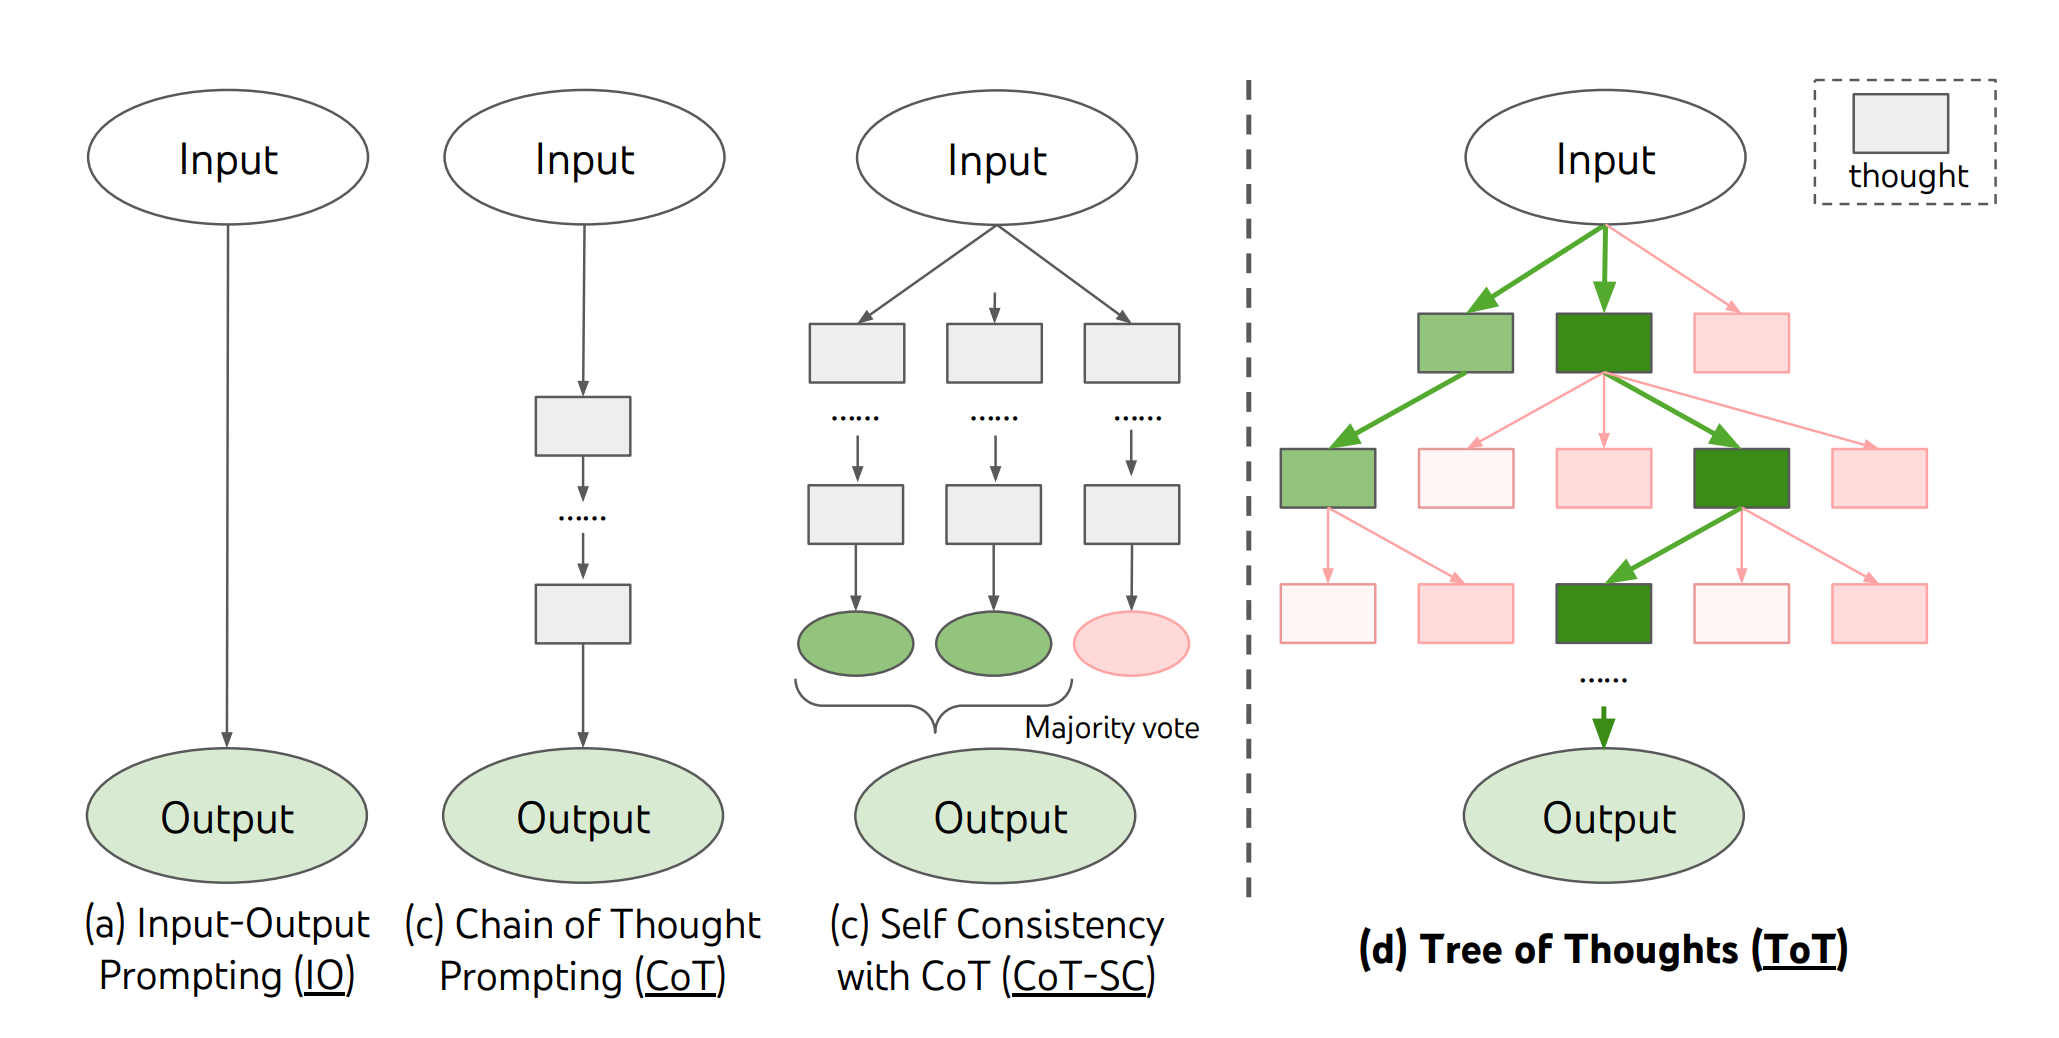
\includegraphics[width=\textwidth]{../images/image024}
					\caption{مقایسه روش \lr{CoT} روش، \lr{sc-CoT} و روش \lr{ToT}}
					\label{CoT_vs_sc-CoT_vs_ToT}
				\end{figure}
				
			\subsection{اعمال \lr{Prompt engineering} روی مدل}
			
				در این پروژه از روش \lr{ToT} برای استدلال در مدل استفاده می‌کنیم چون طببق بررسی‌ها نسخه کامل‌تری از دو روش \lr{CoT} و \lr{sc-CoT} است.
			
			(ارزیابی روش‌ها و انتخاب روش بهتر و اعمال روی مدل و ارزیابی)
				
			
	\chapter{رابط کاربری چت}
			
		در انتها یک رابط کاربری ساده برای تعامل با مدل با استفاده از پکیج \lr{StramLit} ایجاد که طراحی کلی آن را در تصوایر \ref{stramLitAPP1} و \ref{stramLitAPP2} قرار دارد.
		
		\begin{figure}[ht]
			\centering
			
\includegraphics[width=\textwidth]{../images/image004}
			\caption{رابط کاربری ایجاد شده برای تعامل با مدل (تصویر خالی)}
			\label{stramLitAPP1}
		\end{figure}
				
		\begin{figure}[ht]
			\centering
			
\includegraphics[width=\textwidth]{../images/image005}
			\caption{رابط کاربری ایجاد شده برای تعامل با مدل (تصویر همراه با چت)}
			\label{stramLitAPP2}
		\end{figure}
		
		
	\chapter{کارهای بیشتر}
		
		\section{مبدل صوت به متن \lr{(ASR)}}
		
		\section{مبدل متن به صوت \lr{(TTS)}}
		
		\section{مدل‌های \lr{(VLM)}}
			
		\section{\lr{Instruction tuning}}
		
		\section{آموزش کامل مدل \lr{(Pre-training)}}
	
	\chapter{نتیجه گیری}
		
		(جدول کامل مقایسه با مدل‌های فارسی زبان و ارتقاهای هرقسمت)
	
	
	\setLTRbibitems
	\makeatletter
	\bidi@AtBeginEnvironment{thebibliography}{\latinfont}
	\makeatother
	\bibliographystyle{ieeetr}
	\bibliography{../BibTeX/ref}
	


\end{document}